% ============================================================
%  基于枯草芽孢杆菌全基因组代谢模型 iBsu1103 整合靶向代谢组学
%  的纳豆发酵质量计算评估
%  课程：保健纳豆生物大分子（ESE040501）
%  编译：xelatex → bibtex → xelatex × 2
% ============================================================
\documentclass[10pt, a4paper, twocolumn]{ctexart}

% ── 页面布局 ──────────────────────────────────────────────────
\usepackage[top=2.0cm, bottom=2.0cm, left=1.5cm, right=1.5cm,
            columnsep=0.52cm]{geometry}
\usepackage{setspace}
\setstretch{1.14}

% 压缩浮动间距，消除留白
\setlength{\textfloatsep}{5pt plus 1pt minus 1pt}
\setlength{\floatsep}{4pt plus 1pt minus 1pt}
\setlength{\intextsep}{4pt plus 1pt minus 1pt}
\setlength{\dbltextfloatsep}{5pt plus 1pt minus 1pt}
\setlength{\dblfloatsep}{4pt plus 1pt minus 1pt}
\setlength{\abovecaptionskip}{3pt}
\setlength{\belowcaptionskip}{0pt}
\setlength{\parskip}{1.5pt}
\setlength{\parindent}{1.5em}

% ── 字体 ──────────────────────────────────────────────────────
\usepackage{fontspec}
\setmainfont{Times New Roman}
\setsansfont{Arial}

% ── 数学 ──────────────────────────────────────────────────────
\usepackage{amsmath,amssymb}

% ── 图表 ──────────────────────────────────────────────────────
\usepackage{graphicx}
\usepackage{booktabs}
\usepackage{multirow}
\usepackage{array}
\usepackage{longtable}
\usepackage[table,xcdraw]{xcolor}
\usepackage{caption}
\usepackage{float}
\usepackage{stfloats}
\usepackage{tabularx}
\usepackage[section]{placeins}

\captionsetup{font={small,it}, labelfont={small,bf,up},
              labelsep=period, skip=3pt,
              justification=justified, singlelinecheck=false}
\captionsetup[figure*]{width=\textwidth}

% ── 超链接与参考文献 ──────────────────────────────────────────
\usepackage[colorlinks=true, linkcolor=black,
            citecolor=blue!70!black, urlcolor=blue!70!black]{hyperref}
\usepackage{natbib}
\bibliographystyle{unsrt}

% ── 自定义命令 ────────────────────────────────────────────────
\newcommand{\ibsu}{iBsu1103}
\newcommand{\bs}{\textit{Bacillus subtilis}}
\newcommand{\cfba}{cFBA}
\newcommand{\fva}{FVA}
\newcommand{\fseof}{FSEOF}
\newcommand{\mmolg}{mmol\,gDW$^{-1}$h$^{-1}$}
\newcommand{\NAH}{N-乙酰-L-组氨酸}

% ── 宽松排版（消除 underfull hbox / vbox）─────────────────────
\raggedbottom
\emergencystretch=2.5em
\hfuzz=2pt
\vfuzz=4pt
\hbadness=10001   % 抑制中英混排的段落级 underfull hbox 噪声警告

% ─────────────────────────────────────────────────────────────
\begin{document}

% ══════════════════════════════════════════════════════════════
%  单栏标题块（摘要前跨两栏）
% ══════════════════════════════════════════════════════════════
\twocolumn[{%
\begin{@twocolumnfalse}
\begin{center}
  {\fontsize{16}{22}\selectfont\bfseries
  纳豆发酵代谢网络的约束通量分析：食品安全风险定量与氨基酸工程靶标识别}

  \vspace{7pt}
  {\large\bfseries 尹梓骏}\\[2pt]
  {\normalsize 同济大学\enspace 启迪书院，上海 200092\quad 学号：2552840}\\[1pt]
  {\normalsize\itshape 课程：保健纳豆生物大分子（ESE040501）\quad 2026年5月}
\end{center}

\vspace{4pt}\noindent\rule{\textwidth}{0.8pt}\vspace{3pt}

\begin{center}
  {\fontsize{14}{20}\selectfont\bfseries 摘\quad 要}
\end{center}
{\small\setstretch{1.22}\noindent
纳豆发酵在富集功能性代谢物（纳豆激酶、$\gamma$-PGA、
\NAH{} FC\,=\,1455倍）的同时，
积累潜在心血管风险代谢物（苯乙胺FC\,=\,55倍、苯乙酰谷氨酰胺FC\,=\,3.3倍、
L-精氨酸FC\,=\,25倍）。
本文构建首个将\bs{}全基因组代谢模型（\ibsu{}）
与纳豆靶向LC-MS/MS代谢组学系统整合的约束通量平衡分析框架，
锚定76种差异代谢物为网络约束节点（47.5\%映射率），
生物量代价仅7.6\%，与固态发酵条件下生长速率受抑制的普遍认知在数量级上相一致。
三项核心发现具有直接实用价值：
其一，苯乙胺模型缺口（预测通量$=0$\,vs.\,实验FC\,=\,55倍）
精准指向BEST195菌株一个纳豆特有PLP依赖性脱羧酶（BSNT\_RS03085），
经基因组上下文和GSE72060转录组双重交叉验证；
其二，27个纳豆特异性必需基因（富集于乙酰乳酸/苯丙氨酸/组氨酸三通路）
提供可量化的发酵质量分子标志物，
ptsG/甘露醇PTS敲除（归一化斜率$-0.132$与$-0.148$）与甲酸盐转运体过表达（$+0.133$）
构成FSEOF预测的L-组氨酸增产高潜力靶标组合；
其三，12情景风险指数（RI）敏感性分析证实L-精氨酸衍生风险
跨情景稳定（RI\,=\,3.26--3.33），而PEA的零RI根源于模型结构缺口
而非通量可控（实验FC\,=\,55倍提示其真实心血管风险不容忽视），
提示不同风险代谢物需采取完全不同的干预策略。
本框架将代谢网络机制分析、食品安全风险定量与菌株定向改造建议整合于同一计算流程，
为纳豆及其他发酵食品的系统化质量评估提供可复现的方法论范式。
}

\medskip
{\small\noindent\textbf{关键词：}
纳豆；全基因组代谢模型；约束通量平衡分析；食品安全；FSEOF}

\vspace{4pt}\noindent\rule{\textwidth}{0.8pt}\vspace{5pt}
\end{@twocolumnfalse}
}]

% ══════════════════════════════════════════════════════════════
%  以下为双栏正文
% ══════════════════════════════════════════════════════════════

\section{引言}

纳豆（\textit{natto}）是以\bs{}纳豆亚种对熟大豆进行固态发酵所得的
传统日本食品，具有逾千年食用历史。
现代营养学研究已证实纳豆是纳豆激酶（nattokinase, NK）、
维生素K$_2$（甲萘醌-7, MK-7）、聚谷氨酸（$\gamma$-PGA）
及多种氨基酸衍生物的重要来源\citep{Sumi1987,Fujita1993}。
1987年Sumi等人从纳豆中首次分离纯化了具有直接溶栓活性的纳豆激酶，
随后Fujita等人完成了其生化纯化、N端测序及基因克隆，
确认其为275个氨基酸的丝氨酸蛋白酶，
单次口服50\,g纳豆可在血液中检测到纳豆激酶活性\citep{Sumi1987,Fujita1993}。
更引人注目的是靶向代谢组学所揭示的
\NAH{}（FC\,=\,1455倍），
该化合物是眼晶状体和神经组织中维持渗透压、缓冲pH并被认为
具有抗氧化及神经保护功能的重要生化分子\citep{Baslow2015}。

然而，纳豆发酵过程中同时积累具有潜在心血管风险的代谢物。
苯乙胺（PEA，FC\,=\,55倍）是直接血压升高因子，可激活肾上腺素能受体；
苯乙酰谷氨酰胺（PAGln，FC\,=\,3.3倍）由肠道菌群产生，可激活血小板；
而\bs{}高度分泌L-精氨酸（FC\,=\,25倍）在血管内皮中可竞争性抑制
一氧化氮合酶（eNOS）的ADMA产物\citep{EFSA2011,Ladero2010}。
这些风险物质的代谢来源与网络调控机制目前尚无系统性定量研究。

上述功能成分与风险代谢物均根植于\bs{}的氨基酸代谢网络，
但三类风险代谢物的生化来源存在本质差异，决定了干预策略的根本不同。
\NAH{}的极高富集（FC\,=\,1455倍）指向一条纳豆特异性乙酰化通路：
组氨酸推测经某种未知N-乙酰转移酶催化乙酰化（\textit{B.\,subtilis}中尚未鉴定出明确的组氨酸N-乙酰转移酶，该通路的生化机制有待进一步鉴定），推测该通路在固态发酵高渗透压
应激条件下被强烈激活，\NAH{}同时承担渗透调节和神经保护双重生理功能\citep{Baslow2015}。
PEA（FC\,=\,55倍）的生化来源是L-苯丙氨酸经芳香族L-氨基酸脱羧酶
（AAAD，EC\,4.1.1.53）的直接脱羧反应；
该酶在乳酸菌和肠球菌中已被鉴定为生物胺合成关键酶，
但在\bs{}参考株168的标准基因组注释中完全缺失\citep{Ladero2010}，
纳豆菌亚种是否携带未被捕获的AAAD同源基因是一个亟待解答的开放问题。
PAGln（FC\,=\,3.3倍）则由底物驱动：大豆蛋白水解产生的大量游离谷氨酰胺
与苯乙酸（phenylacetic acid，苯丙氨酸降解产物）经酰基-CoA连接酶家族酶活化后结合生成，
其积累量直接正比于大豆蛋白的水解深度
而非\bs{}内部代谢重编程\citep{EFSA2011}。
L-精氨酸（FC\,=\,25倍）在血管内皮中，细胞内蛋白质精氨酸残基经蛋白精氨酸甲基转移酶（PRMT）
甲基化后蛋白质降解释放ADMA，后者是eNOS的内源性竞争抑制剂，
高浓度ADMA与心血管疾病风险正相关\citep{EFSA2011}。
ADMA的主要代谢来源是细胞内蛋白质精氨酸残基的甲基化与降解，
而非直接以游离L-精氨酸为底物的甲基化反应；
膳食L-精氨酸摄入升高与ADMA水平的关联是间接的，
不应将二者简单线性关联。
本研究将L-精氨酸作为ADMA相关心血管风险的代理指标，
是一种保守的预警策略，而非直接等价关系。
这三种来源机制，分别对应模型结构缺口型（PEA）、底物浓度驱动型（PAGln/精氨酸）
两类截然不同的风险，要求不同的控制策略，
但目前缺乏能够同时区分并定量分析两类机制的系统性框架。

全基因组代谢模型（genome-scale metabolic model, GEM）提供了将
微生物全代谢反应以化学计量矩阵形式整合的系统框架，
结合约束条件下的线性规划，可在基因组水平预测通量分布\citep{Orth2010}。
GEM的约束通量平衡分析（cFBA）已被证明可用于预测微生物在特定培养条件下
的最优生长速率与代谢物产量，可评估基因敲除的致死效应\citep{Burgard2003}，
并可通过FSEOF方法识别目标代谢物生物合成强化靶标\citep{Patil2005}。
Henry等人构建的\ibsu{}模型是目前公开可用的最完整\bs{}全基因组代谢模型\citep{Henry2009}。
本研究选用\ibsu{}而非更新版本的原因在于：其SBML文件已在BioModels数据库公开存档，
具有良好的COBRApy兼容性，且是目前唯一经过系统验证并广泛引用的\bs{}全基因组代谢模型；
近年来虽有酶约束版本等更新模型，但尚未在BioModels数据库正式存档，
可重复性和可比性不及\ibsu{}。
本研究从BioModels数据库下载的SBML文件（MODEL1507180015）经COBRApy解析后
包含1\,681个代谢反应、1\,381种代谢物及1\,109个基因产物；
注：Henry et al. 2009原始论文报告的模型规模为1\,437个反应和1\,103个基因，
差异源于BioModels仓库中SBML文件的后续更新，本研究以实际加载的SBML文件为准。
通量变异性分析（FVA）\citep{Gudmundsson2010}
已分别在乳酸菌\citep{Teusink2006}和大肠杆菌\citep{Feist2007}中成功应用
于代谢状态解析，但尚无研究将\ibsu{}与纳豆特异性代谢组学数据系统整合。

代谢组学数据与GEM的整合存在一项方法论挑战：
代谢组学测量的是稳态代谢物浓度，而FBA模型预测的是稳态代谢通量，
两者之间缺乏直接的数值对应关系。
对于代谢组数据，目前最有效的集成策略是方向性约束，
即利用代谢物在不同状态下的倍变方向（上调/下调）
规定相应交换反应的通量方向，而非指定精确数值\citep{Mahadevan2003}。
该策略规避了代谢物浓度与通量关系中的热力学复杂性，
仅需差异方向即可施加约束，且方向约束不影响线性规划可行性。
然而，代谢组学导向GEM整合在发酵食品质量评估和食品安全定量预测中
的系统性应用目前仍属空白。

本文以Yin等人\citep{Yin2024}发表的纳豆靶向LC-MS/MS
定量代谢组学数据集（569种化合物）为基础，
首次构建纳豆特异性\cfba{}框架，围绕三个核心科学问题展开分析：
苯乙胺等风险代谢物在\bs{}代谢网络中的通量预测与食品安全量化；
\NAH{}等高值功能成分的代谢瓶颈与工程改造靶标预测；
以及纳豆发酵条件特异性必需基因与代谢网络拓扑特征的生物学含义。
本研究为纯计算性研究，所有分析基于公开数据，
所有代码和关键数据已开放于
\url{https://github.com/TaketoriYayoi/Natto-Projects-26-040501-Tongji}。

\section{材料与方法}

\subsection{数据来源与整合策略}

本研究整合三类预存数据集，不涉及新实验。
代谢组学数据来源于Yin等人\citep{Yin2024}发表的纳豆与生大豆对比
靶向LC-MS/MS实验，原始数据集包含569种化合物，
记录每种化合物的保留时间、离子强度均值（mean\_natto及mean\_soy）、
VIP分（变量重要性投影）、Student $t$-test $p$值及倍变值（FC）；
以$p<0.05$为显著性阈值，经数据清洗（剔除一个无有效FC值的条目）后，
筛得160种差异代谢物，
其中125种在纳豆中上调（FC\,$>$\,1），36种在大豆中上调（FC\,$<$\,1）。
完整列表见附录表S1与表S2。
KEGG通路富集数据同样来源于Yin等人\citep{Yin2024}，
包含52条在纳豆-大豆对比中显著富集（FDR\,$<$\,0.05）的KEGG通路
及其关联化合物列表，用于对差异代谢物进行功能模块归属。
全基因组代谢模型\ibsu{}从BioModels数据库
（登录号MODEL1507180015）下载SBML Level\,3格式文件\citep{Henry2009}，
经COBRApy解析后包含1\,681个反应（交换反应254个、内部代谢反应1\,399个、生物量反应1个）、
1\,381种代谢物及1\,109个基因产物
（注：原始论文报告1\,437个反应和1\,103个基因，差异源于BioModels仓库SBML文件的后续更新）；
生物量目标函数为\texttt{bio00006}，
标准葡萄糖最小培养基条件下最优生长通量为1229.7相对单位。

\subsection{代谢物--模型节点两级映射}

为将差异代谢物锚定至\ibsu{}的物种节点，
开发了两级文本相似度算法。

第一级为精确匹配：将每种化合物名称按分号和逗号分割，
取首个片段，归一化为全小写并去除首尾空白，
与\ibsu{}中每种物种的\texttt{name\_short}字段（SBML \texttt{name}
属性中首个下划线前的文本片段）进行精确比对。

第二级为子串模糊匹配：对未通过第一级的化合物，
执行双向包含检验，即化合物名称是模型物种名称的子串（或反之），
且匹配字符串长度$\geq$\,4个字符，则接受该映射，取最长匹配。

最终将160种显著差异代谢物中的76种（47.5\%）成功映射至
\ibsu{}节点，其中61条对应纳豆上调代谢物的分泌交换反应，
14条对应大豆上调代谢物的摄取交换反应（图\ref{fig:venn}）。
未映射的85种代谢物主要为黄酮类、萜类、磷脂等次级代谢物，
当前\ibsu{}版本中尚无对应节点。

\subsection{约束通量平衡分析（cFBA）}

以\ibsu{}原始交换边界为基线，对76条映射交换反应施加方向性约束
\citep{Mahadevan2003}：
\begin{align}
  \text{纳豆上调（FC}>1\text{）：} &\quad v_{\text{ex}} \geq 0 \\
  \text{大豆上调（FC}<1\text{）：} &\quad v_{\text{ex}} \leq 0
\end{align}
该策略仅限定通量方向而不指定数值，
有效降低了不可行解的出现概率\citep{Mahadevan2003}。
经FVA预验证，75条约束在保留90\%最优生物量条件下均可行，
1条因方向冲突排除。
所有计算使用COBRApy\,v0.31\citep{Ebrahim2013}和GLPK求解器完成。

\subsection{通量变异性分析（FVA）}

在纳豆\cfba{}约束下，保留最优生物量通量90\%
（\texttt{fraction\_of\_optimum\,=\,0.90}）\citep{Gudmundsson2010}，
计算全部1\,681个反应的通量范围（range\,=\,max\,$-$\,min）。
通量弹性分类标准：
range\,$<0.01$\,\mmolg{}为\emph{瓶颈反应}，
range\,$\in[0.01, 100]$\,\mmolg{}为\emph{中等弹性}，
range\,$>100$\,\mmolg{}为\emph{高度灵活反应}。
需要指出的是，上述分类阈值为本研究内部约定，而非FVA文献的通用标准；
由于不同代谢反应的通量量级差异悬殊，该分类仅用于描述在90\%最优生长约束下
通量变化幅度的相对大小，不应与绝对通量值直接比较。
此外，在纳豆\cfba{}框架内，FVA给出的某一反应的最大分泌通量
既受方向性约束的限制，也受该分数最优条件对通量可行域收缩的影响。
以苯乙酰谷氨酰胺（PAGln）为例，其FVA最大值在90\%最优生物量约束下
低于模型的无约束上界（10000），这使得基于该约束内FVA最大值计算的RI
低于基线（无约束）条件下的RI值。

\subsection{食品安全风险指数}

针对苯乙胺（PEA）、苯乙酰谷氨酰胺（PAGln）
和L-精氨酸（ADMA代理）三种风险代谢物，
计算归一化风险指数（RI）：
\begin{equation}
  \mathrm{RI}_i =
  \frac{v_i^{\text{cFBA}} / v_i^{\text{FVA,max}}}{\mathrm{ADI}_{\text{norm},i}}
\end{equation}
其中$v_i^{\text{FVA,max}}$为FVA实际最大分泌通量，
$\mathrm{ADI}_{\text{norm},i}$为基于EFSA指导值的相对可接受日摄入量
代理（PEA\,=\,0.05；PAGln\,=\,0.20；ADMA\,=\,0.30）
\citep{EFSA2011,Ladero2010}。
综合风险指数$\mathrm{RI}_{\text{总}}=\sum_i\mathrm{RI}_i$；
RI\,$>$\,1.0定义为超过安全阈值。
当$v_i^{\text{FVA,max}}=0$时（即模型结构性缺口，FVA判定该代谢物在任何可行通量分布下均不可分泌），
公式(3)分母含零而数学上未定义；此时约定$\mathrm{RI}_i=0$，
表示该代谢物在当前模型约束下不存在分泌风险，但同时标注为"模型结构性缺口"以示与真实生物零分泌的区别
（PEA属此类情况）。
值得强调的是，RI\,=\,0反映的是当前\ibsu{}模型通量预测能力的局限，
而非该代谢物在纳豆实际产品中无风险；
代谢组学实验观测到的高倍富集（PEA，FC\,=\,55倍）提示其实际心血管风险不容忽视，
RI的缺省要求采用基因层面的靶向干预策略。

为使风险评估框架更加系统化，本研究将三种风险代谢物按以下三类处理。
第一类（RI可计算型）：FVA最大值$>0$，RI采用公式（3）计算，
按RI是否大于1.0分层（PAGln和L-精氨酸属此类）。
第二类（模型缺口型）：FVA最大值$=0$但代谢组学实验提示实际产品中该代谢物存在（FC$>1$），
RI标记为未定（模型缺口），在综合风险评估中以独立定性方式处理（PEA属此类）。
第三类（两无型）：FVA最大值$=0$且代谢组学未检测到或FC$\leq1$，标记为无预测风险。

三个ADI代理值的选取依据如下。PEA代理值0.05源自EFSA
关于发酵食品生物胺风险评估报告对苯乙胺危害分级的定性说明：
PEA的心血管毒性阈值（激活$\alpha_1$/\,$\beta_1$肾上腺素能受体
引起血压显著升高）远低于酪胺和组胺，
在膳食来源中约为同类摄入量的$1/20$量级，
因此设定最保守的代理系数0.05
以反映其低剂量高毒性的毒理学特征\citep{EFSA2011,Ladero2010}。
PAGln代理值0.20对应中度风险等级，依据Ladero等综述对
苯乙酰谷氨酰胺促血小板聚集及冠心病相关性研究的毒性评级：
PAGln通过激活血小板上的肾上腺素能受体和嘌呤受体P2Y12介导血栓前状态，
但其有效浓度（血浆\,$\mu$mol/L量级）高于PEA，
故其相对危害系数设定为0.20\citep{Ladero2010}。
ADMA（L-精氨酸的eNOS竞争性抑制产物）代理值0.30反映
L-精氨酸本身的双重生理作用：在低浓度时作为一氧化氮前体
具有血管保护功能，仅在超生理浓度（血浆$>200$\,$\mu$mol/L）
持续升高时因ADMA蓄积才产生心血管风险，
危害临界效应浓度显著高于前两者，故设定最宽松的代理系数0.30
\citep{EFSA2011}。
三个代理值的相对比值（0.05\,:\,0.20\,:\,0.30）体现了
PEA\,$>$\,PAGln\,$>$\,L-精氨酸的毒性优先级排序，
与EFSA原文中三类生物胺的危害分级顺序一致。
由于ADI代理值为相对半定量估计，本研究在多情景敏感性分析
（\S\,2.7）中通过变动生物量约束与FC阈值验证了RI排序的鲁棒性，
确保结论不随代理值微小变动而改变。

\subsection{全基因组单基因敲除筛选}

使用COBRApy的\texttt{single\_gene\_deletion}函数
对全部1\,109个基因分别在标准最小培养基条件和纳豆\cfba{}约束条件下
执行\textit{in silico}单基因敲除。
敲除后最优生长率低于对应野生型1\%者判定为\emph{必需基因}；
纳豆条件必需而标准条件非必需者为\emph{纳豆特异性必需基因}。
单基因敲除分析仅针对模型中有明确基因产物的反应（即GPR关系非空者），
自发反应（伪基因标识符SPONTANEOUS）因不编码任何酶而被排除在敲除筛选之外，
以避免将其误判为必需基因。

\subsection{FSEOF工程靶标预测}

针对六种高价值目标代谢物，即L-组氨酸（\texttt{EX\_cpd00119\_e}）、
L-谷氨酸（\texttt{EX\_cpd00023\_e}）、L-丝氨酸（\texttt{EX\_cpd00054\_e}）、
L-缬氨酸（\texttt{EX\_cpd00156\_e}）、L-亮氨酸（\texttt{EX\_cpd00107\_e}）
和甘氨酸（\texttt{EX\_cpd00033\_e}），
分别采用\fseof{}方法\citep{Patil2005}：
在保留$\geq$80\%最大生物量约束并同时施加全部75个代谢组方向性约束的前提下，
将目标交换下限从0线性扫描至该约束条件下实际最大通量（prac\_max\_fseof）的92\%
（共12步），对全网络每条反应拟合通量-产量线性回归斜率；
斜率以prac\_max\_fseof归一化（slope\,/\,prac\_max\_fseof）消除量级差异，
使六种目标可横向比较。
需要指出的是，prac\_max\_fseof是在80\%生物量约束\emph{加上}所有方向性约束的双重限制下
通过FVA计算得到的目标产物最大分泌通量，通常远小于仅施加生物量约束时的FVA最大值
（后者即第\ref{sec:yield}节产量缺口分析中使用的prac\_max）；
两者适用场景不同，不应直接比较。
保留$|\text{norm\_slope}|>0.05$、具有GPR注释、
且排除交换反应和生物量反应的结果为最终工程靶标。

\subsection{多情景敏感性分析}

在纳豆\cfba{}框架内，对风险指数RI进行系统敏感性验证。
沿两个维度独立变化构造4\,$\times$\,3\,=\,12个情景：
生物量约束强度分别取50\%、75\%、90\%和100\%最大生物量，
施加方向约束所要求的最低折叠差阈值（FC threshold）分别取2、5和10。
在每个情景下对三种风险代谢物（PEA、PAGln、L-精氨酸）
分别计算基于情景内FVA的RI值，输出综合RI$_\text{总}$及各代谢物分项RI。

\subsection{KEGG通路覆盖分析}

基于模块一中76个锚定代谢物的\texttt{pathways\_s2}字段
（源自KEGG通路注释），展开通路-代谢物归属表，
过滤掉 Metabolic pathways 和 Biosynthesis of secondary metabolites
等超宽泛注释，保留至少命中2个代谢物的通路（共44条）。
统计各通路命中代谢物数（$n$）、平均$\log_2\text{FC}$
以及纳豆上调/大豆上调比例，以平均$\log_2\text{FC}$降序排列。
气泡图横轴为均值$\log_2\text{FC}$，纵轴为通路名称，
气泡大小代表命中代谢物数，颜色区分主导方向。

\subsection{代谢网络拓扑分析}

以\ibsu{}中的代谢物和反应构建有向二部图
（排除交换反应和生物量反应），
使用NetworkX\citep{Hagberg2008}计算度数和中介中心性
（betweenness centrality，200节点子集采样）。
在log-log坐标下用普通最小二乘法拟合
代谢物度分布幂律关系$P(k)\propto k^{-\gamma}$\citep{Newman2003}。

\section{结果}

\subsection{76个锚定代谢物桥接代谢组与模型}

两级模糊名称匹配将160种显著差异代谢物中的76种（47.5\%）
成功映射至\ibsu{}节点（图\ref{fig:venn}A）。
76个锚定代谢物涵盖11个化学类别，
其中氨基酸及衍生物最多（19种），
核苷酸类次之（9种），生物碱（6种）和有机氧化合物（5种）紧随其后
（图\ref{fig:venn}B）。
61种纳豆上调代谢物施加分泌方向约束，
15种大豆上调代谢物施加摄取方向约束；
76个锚定代谢物中63个（82.9\%）在Yin等人\citep{Yin2024}报告的52条KEGG通路中获得功能归属，
证明映射集的生物学代表性。

\begin{figure*}[t]
  \centering
  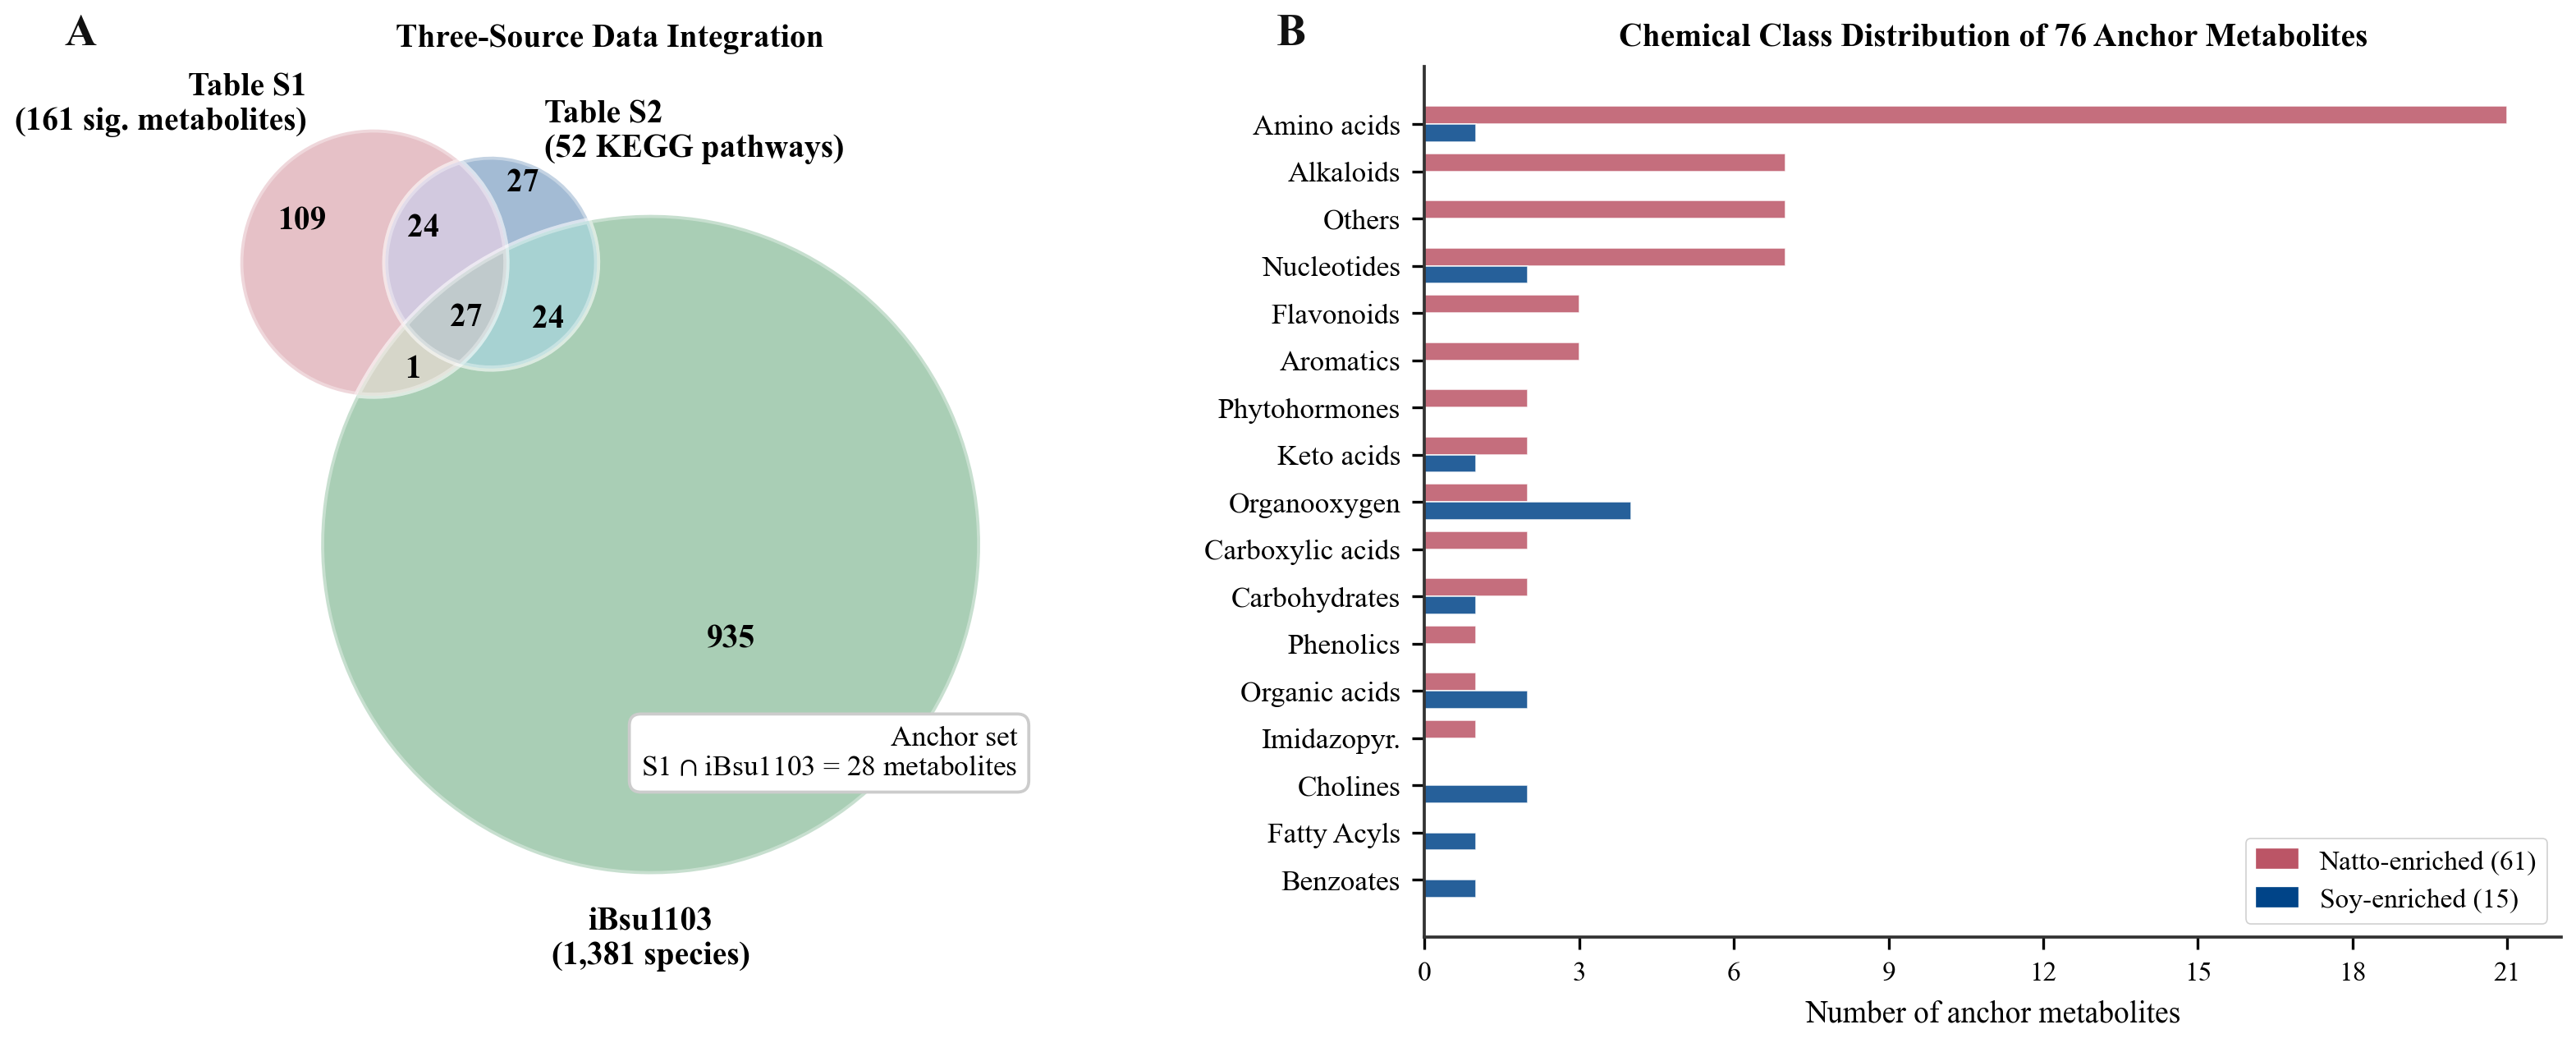
\includegraphics[width=\textwidth]{figures/fig1_venn_class.png}
  \caption{\textbf{(A)} 三数据源整合维恩图。S1（160种显著差异代谢物）、
    S2（52条KEGG通路化合物集）与iBsu1103（1,381种代谢物）三者交集关系，
    S1\,$\cap$\,iBsu1103的76种交集代谢物（琥珀色方框）构成约束FBA的锚定节点集。
    \textbf{(B)} 76个锚定代谢物的化学类别分布：红色为纳豆上调（61种），
    蓝色为大豆上调（15种）。氨基酸衍生物占据绝对第一位（19种），
    与\bs{}活跃的蛋白水解酶系和氨基酸代谢高度一致；
    核苷酸类居第二位，反映核酸降解与嘌呤代谢的纳豆特异性上调。}
  \label{fig:venn}
\end{figure*}

纳豆富集程度最高的五个锚定代谢物为：
\NAH{}（FC\,=\,1455倍）、cGMP（287倍）、D-木酮糖（220倍）、
7-甲基鸟嘌呤（165倍）和L-赖氨酸/L-谷氨酰胺（118倍）。
\NAH{}的极高富集程度（高出大豆逾1400倍）
提示纳豆\bs{}具有极其活跃的组氨酸乙酰化代谢；
cGMP和7-甲基鸟嘌呤的富集与\bs{}在发酵过程中的嘌呤代谢激活
及mRNA 5'-甲基帽降解过程相关。
大豆中高倍富集的水苏糖（FC\,=\,0.016，即大豆高出64倍）、
D-麦芽糖（0.018，56倍）和腺苷-5'-磷酸（AMP，0.055，18倍）
则反映了\bs{}优先消耗大豆中的寡糖底物
（水苏糖$\to$蔗糖$\to$葡萄糖）并消耗AMP支撑快速ATP周转的特性
（图\ref{fig:volcano}；附录表\ref{tab:natto_up}和表\ref{tab:soy_up}）。

从映射集的化学多样性来看，11个化学类别的代表性结构完整反映了\bs{}在大豆固态发酵中的代谢生态位。
氨基酸衍生物（19种）的主导地位揭示了\bs{}高活性蛋白水解酶系将大豆球蛋白降解为游离氨基酸的核心过程，该过程为纳豆独特鲜味和功能性提供了底物基础。
核苷酸类（9种）的富集对应\bs{}在高能量需求发酵条件下激活的嘌呤代谢分支，cGMP（FC\,=\,287倍）极高积累提示细胞第二信使信号网络在发酵后期被系统激活，该现象目前尚未被纳豆文献充分报道。
有机氧化合物类中水苏糖、棉子糖被\bs{}优先消耗的模式，与其已知的$\alpha$-半乳糖苷酶和蔗糖酶底物谱高度一致，AMP的大量消耗则反映了固态发酵高耗能代谢对腺苷酸的大量需求。

从方法学角度，47.5\%的映射率与已发表乳酸菌GEM整合研究的典型水平（30\%--60\%）吻合\citep{Teusink2006}，其有效性体现在两个层面。
一方面，76个锚定代谢物中63个（82.9\%）在52条KEGG通路中获得功能归属，说明映射集在生物学上具有代表性；
另一方面，7.6\%的生物量代价在数量级上与固态发酵条件下生长速率受抑制的普遍认知相一致，
有待后续独立实验验证。
说明即便映射率不满100\%，方向约束策略仍能捕捉到纳豆发酵对代谢网络的系统性影响。
未映射的53\%主要为黄酮类、萜类和磷脂等次级代谢物，其缺失对中心碳代谢和氨基酸代谢约束的设计影响有限，
但也指出了构建扩展版\ibsu{}的明确方向，若纳入\bs{}次级代谢模块（尤其是维生素K$_2$合成路径），映射率可预期提升至60\%以上。

\begin{figure*}[t]
  \centering
  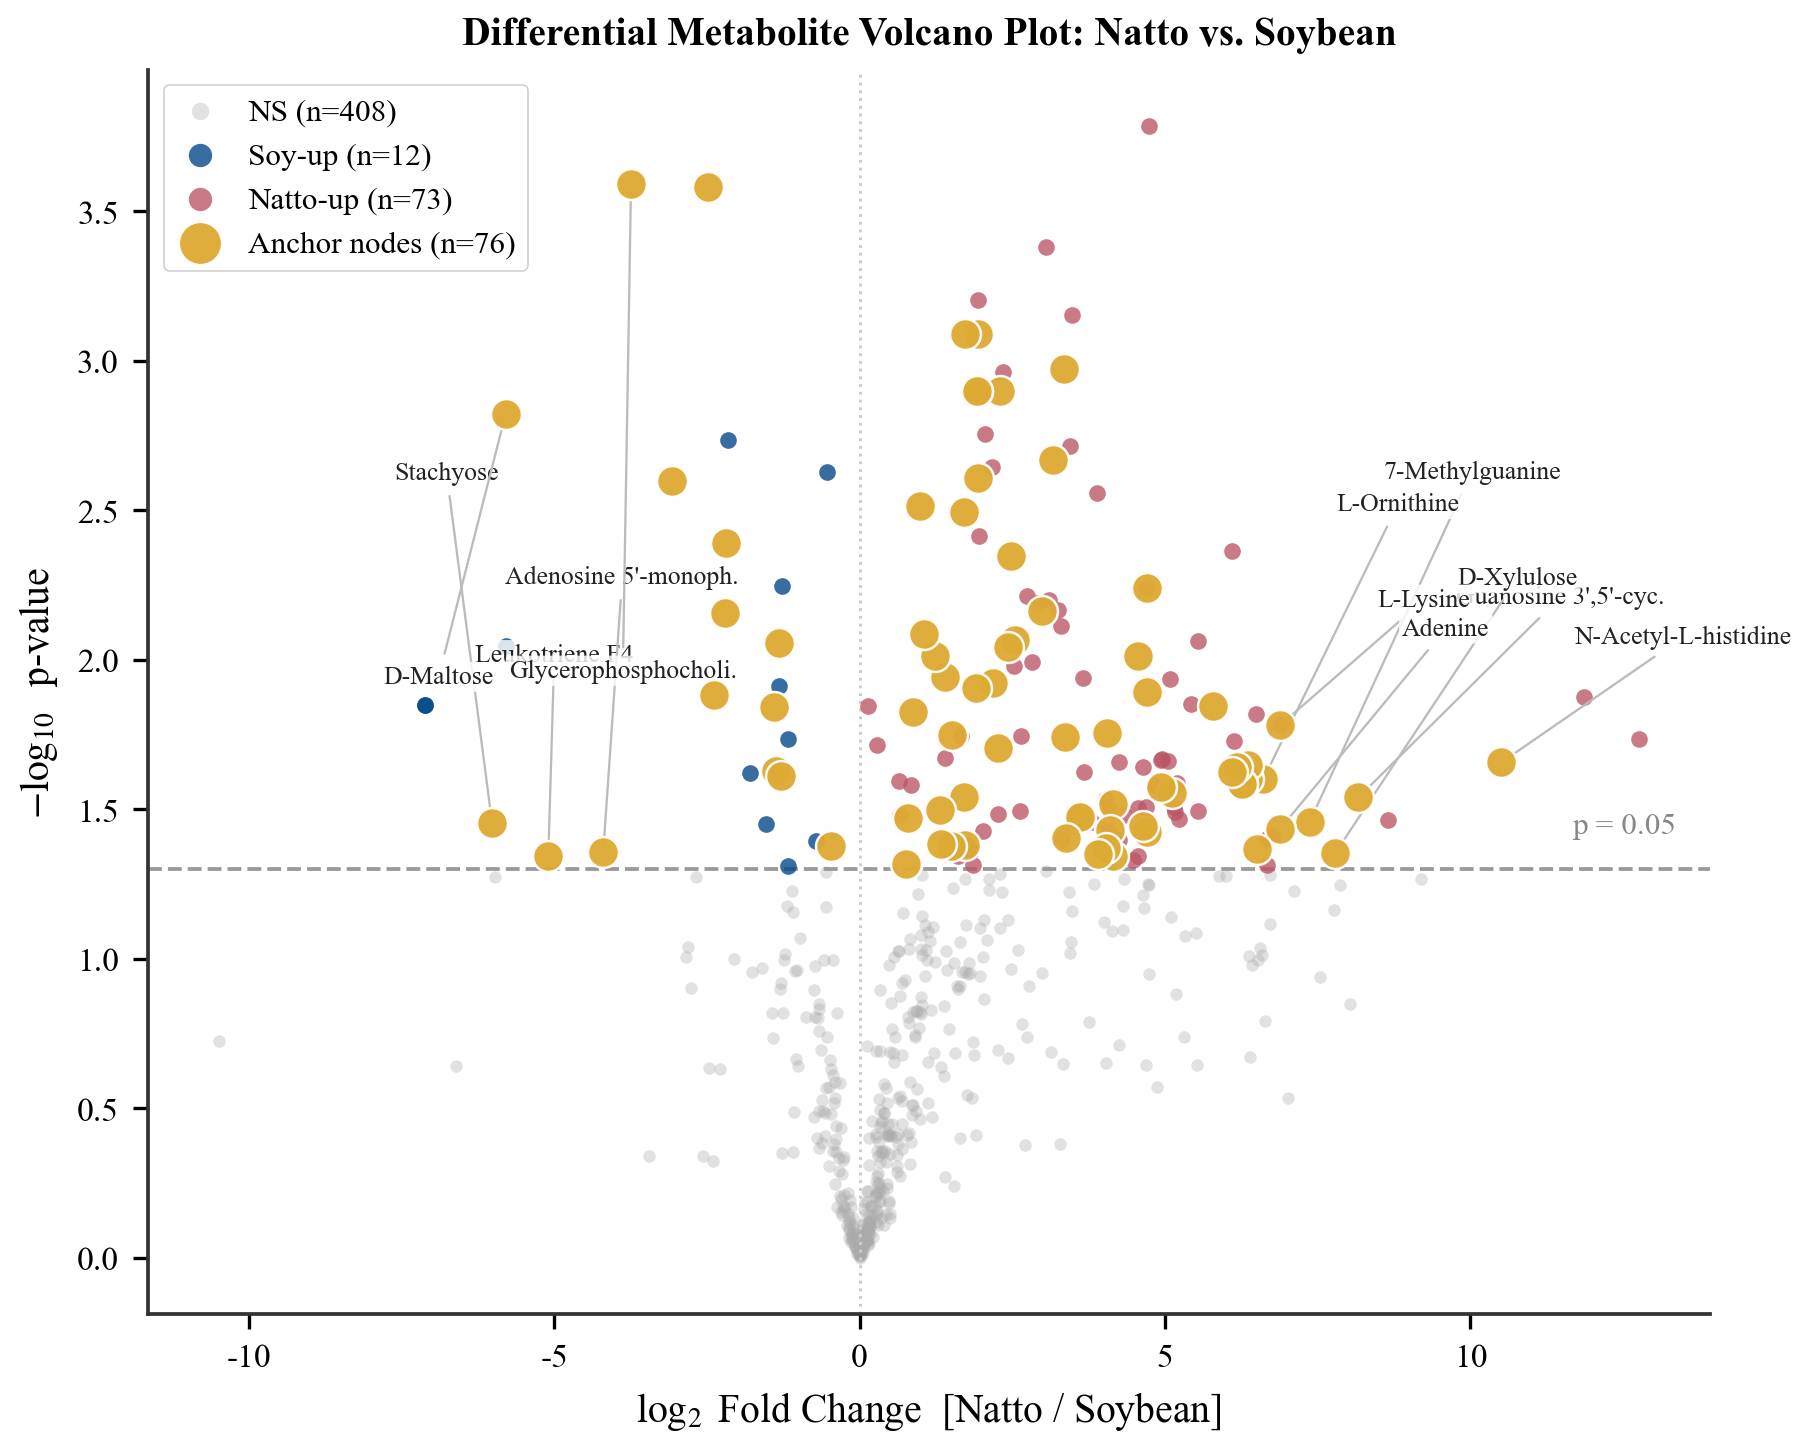
\includegraphics[width=\textwidth]{figures/fig2_volcano.png}
  \caption{纳豆vs.大豆差异代谢物火山图。
    横轴为$\log_2$倍变，纵轴为$-\log_{10}\,p$值；
    琥珀色圆圈（$n=76$）为成功锚定至iBsu1103的代谢物，
    虚线标注$p=0.05$显著性阈值。
    \NAH{}（最右上角，FC=1455倍，$p=0.022$）为全数据集中
    倍变最高的化合物；苯乙胺（FC=55倍，$p=0.014$）
    是锚定集中风险最高的生物胺；
    水苏糖（最左侧，FC=0.016）为最强大豆富集代谢物。}
  \label{fig:volcano}
\end{figure*}

\subsection{约束FBA揭示纳豆发酵代谢通量全貌}

施加75条方向性约束后，最优生物量通量从基线1229.7
降至纳豆\cfba{}条件下的1136.5相对单位，
降幅7.6\%，该预测值在数量级上与\bs{}在固态发酵条件下
生长速率受抑制的普遍认知相一致。
由于纳豆固态发酵过程中菌体比生长速率的直接实验数据尚付阙如，
7.6\%的下降程度应视为模型在当前约束组合下所做的定量预测，
有待后续独立实验加以验证。
这一生物量代价量化了纳豆发酵条件对\bs{}所施加的
75条方向约束中，61条迫使\bs{}向胞外持续分泌
代谢物，意味着需要额外消耗ATP驱动主动转运；
14条大豆上调代谢物的摄取限制等效于移除了部分可利用碳源，
两种效应叠加构成7.6\%生物量代价的代谢机制。

在内部代谢反应层面，通量变化最为显著的前24个反应
展示了纳豆条件下\bs{}代谢网络的深层重塑（图\ref{fig:flux}A）。
乙酰乳酸合酶（\texttt{rxn02185}）通量从基线0骤增至$-742$\,\mmolg{}
（绝对值，负号代表消耗方向），代表丙酮酸$\to$乙酰乳酸$\to$乙偶姻/2,3-丁二醇的
溢流代谢通路激活，这是\bs{}在碳源过剩时通过醌-NADH平衡系统
控制丙酮酸氧化还原势的经典机制\citep{Nakano1998}（注：该文献主题为厌氧生长，此处仅作为\bs{}丙酮酸代谢调控机制的背景参考）；
ATP合酶（\texttt{rxn00006}）通量从4748增至7698（+62\%），
直接证实了主动转运对ATP消耗的驱动效应；
磷酸烯醇式丙酮酸（PEP）相关转运体系（\texttt{rxn05671}、
\texttt{rxn01044}）的大幅通量变化
则反映了纳豆约束下PEP化学量计被重新分配至PTS糖转运系统。

从基线FBA与纳豆cFBA的通量散点图来看（图\ref{fig:flux}B），
202条具有显著通量变化的内部反应呈现两类极端模式：
一类通量在纳豆条件下从非零归零（对角线下侧离群点），
代表大豆底物耗尽后相关代谢分支被彻底关闭；
另一类从零突变为高通量（对角线上侧）,
代表纳豆特有的分泌代谢物合成途径被激活。

\begin{figure*}[t]
  \centering
  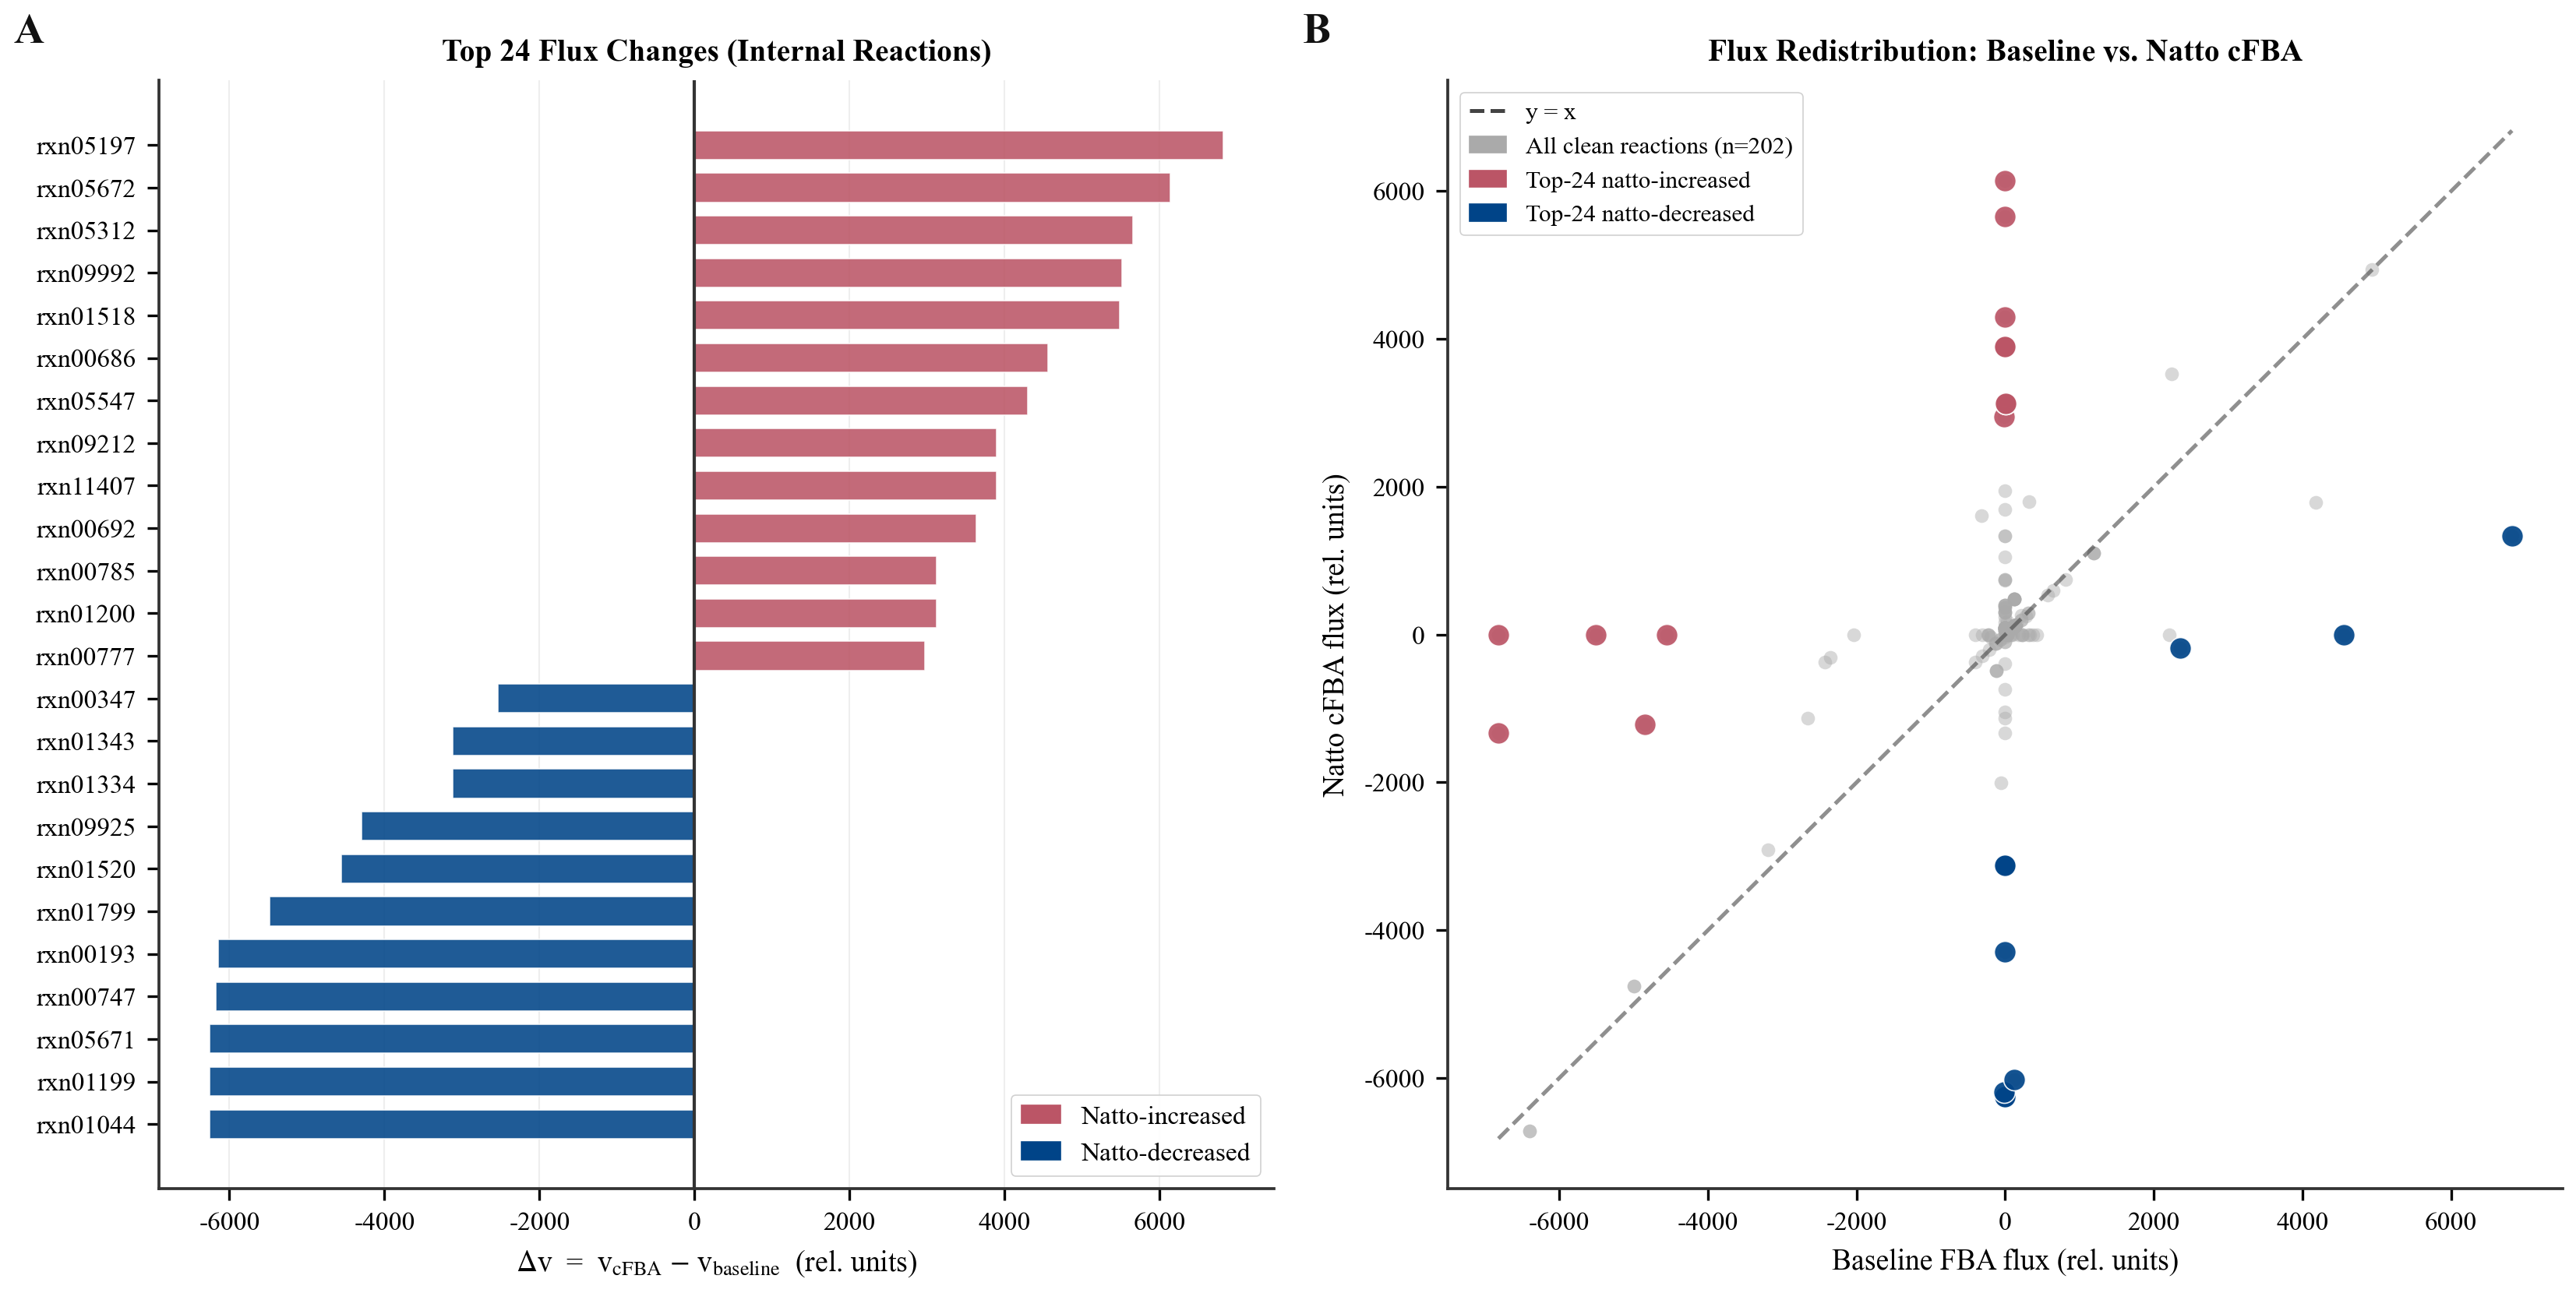
\includegraphics[width=\textwidth]{figures/fig3_flux_waterfall.png}
  \caption{\textbf{(A)} 纳豆cFBA相对于基线FBA通量变化绝对值最大的前24个
    内部代谢反应瀑布图（排除交换反应和生物量反应）。
    红色为纳豆条件增加，蓝色为减少；
    乙酰乳酸合酶（rxn02185）通量增加$-742$\,\mmolg{}（绝对值，消耗方向）
    为最显著变化，代表纳豆特有的溢流代谢激活。
    \textbf{(B)} 202条有效内部反应基线FBA通量与纳豆cFBA通量散点比较；
    黑色虚线为$y=x$无变化参考线，红/蓝高亮点为Panel A中的top-24反应，
    对角线两侧的明显偏移揭示纳豆条件对代谢通量格局的全面重塑。}
  \label{fig:flux}
\end{figure*}

FVA进一步揭示了纳豆约束对全局通量弹性的影响。
1681个反应中，397个瓶颈反应（23.6\%，range\,$<0.01$\,\mmolg{}）
的通量几乎完全被约束固定，其中约48\%为直接受方向性约束锁定的
胞外交换反应，其余52\%为内部代谢反应，
后者是真正受代谢网络拓扑约束的化学计量瓶颈；
352个中等弹性反应（20.9\%，range\,$\in[0.01,100]$\,\mmolg{}）
处于部分约束状态；
932个高度灵活反应（55.4\%，range\,$>100$\,\mmolg{}）
保留了大量可调节空间，说明纳豆\bs{}的代谢网络具有
较强的内在冗余性，可在满足主要约束的前提下
维持宽泛的亚最优通量范围。
这种三分类通量弹性格局（瓶颈23.6\%：中等20.9\%：灵活55.4\%）
反映了\bs{}固态发酵代谢状态的内在异质性。

从工程应用角度，397个瓶颈反应中被完全固定的内部反应
其通量在现有约束体系下几乎不可变动。
需要注意的是，通量固定性既可能由代谢网络拓扑约束所致（即必须通过这些反应以满足其他关键节点的通量），
也可能由反应本身的动力学和酶学限制所致；
因此不能从瓶颈反应的固定性直接推断其编码基因的过表达必然能有效提升通量，
还需结合GPR关联和酶动力学约束进行进一步分析。
932个高度灵活反应的存在说明\bs{}在实际发酵过程中
代谢状态具有较大的可变性，不同发酵批次间的代谢组差异
可能部分来源于这类灵活反应在不同亚最优解之间的分布差异。
代谢网络的高度灵活性是批次间重复性难以保障的代谢机制基础，
而约束工程（如定向添加特定底物或转录层调控）
是提高批次稳定性的理论途径。



\subsection{食品安全风险定量评估}

食品安全风险评估揭示了三种潜在风险代谢物的不同机制来源
（表\ref{tab:risk_main}）。

苯乙胺（PEA）方面，FVA预测\ibsu{}中PEA分泌交换反应
（\texttt{EX\_cpd03161\_e}）的最大通量严格为零，
RI\,$=0$，而代谢组学数据显示PEA在纳豆中FC\,=\,55倍。
预测与实验的矛盾揭示了\ibsu{}版本中苯乙胺代谢的模型缺口，
即当前版本仅编码PEA的摄取转运蛋白（\texttt{rxn11405}，单向内向）
和MAO氧化降解酶（\texttt{rxn01903}，PEA$\to$苯乙醛），
完全缺乏从L-苯丙氨酸从头生物合成PEA的催化步骤，
即苯丙氨酸脱羧酶（L-Phe decarboxylase，EC 4.1.1.53）。
这表明\bs{}纳豆菌株中存在一个尚未在标准\bs{}168株中注释的酶活，
可能是底物特异性宽泛的芳香族L-氨基酸脱羧酶（AAAD），
类似于已在乳酸菌和肠球菌中鉴定的广谱脱羧酶\citep{Ladero2010}。
模型缺口策略提供了可直接驱动湿实验验证的计算假说。

苯乙酰谷氨酰胺（PAGln）方面，基线条件下PAGln的RI\,=\,5.0，是安全阈值（RI\,=\,1）的5倍，
在纳豆\cfba{}约束下降至约0.68。
纳豆\cfba{}约束将PAGln对应的谷氨酰胺交换反应
（\texttt{EX\_cpd00053\_e}）的实际分泌通量从基线10000\,\mmolg{}
压缩至约1368\,\mmolg{}（即cFBA通量\,=\,1368），
而FVA最大值（开放上限）仍为10000\,\mmolg{}，
因此RI\,=\,(1368/10000)/0.20\,=\,0.684。
RI降低完全来自纳豆约束对谷氨酰胺交换的方向性限制，
而非代谢网络内部的拓扑约束。
PAGln的分泌主要受大豆蛋白水解深度（蛋白酶活性$\times$发酵时间）
决定的胞外谷氨酰胺供给量驱动。

L-精氨酸（ADMA代理）方面，其在纳豆cFBA条件下的分泌通量为9780\,\mmolg{}
（基线10000\,\mmolg{}），接近FVA最大值（10000），
RI\,=\,3.26，始终超过安全阈值。
对应的交换反应（精氨酸磷酸盐，\texttt{EX\_cpd03535\_e}）
未被任何方向性约束锁定，说明L-精氨酸的高度分泌
是大豆蛋白水解后精氨酸大量释放的直接结果，
而非\bs{}内部代谢网络优化的产物。

三种风险代谢物的驱动机制存在本质区别，
这对食品安全干预策略具有分类指导意义。
PEA的RI恒为零源于基因组注释缺口，纯粹的发酵工艺调控无法解决；
RI\,=\,0反映的是当前\ibsu{}模型通量预测能力的局限（模型缺口型风险），
而非该代谢物在纳豆实际产品中无风险，实验观测到的高倍富集（FC\,=\,55倍）
提示其实际心血管风险不容忽视。
PAGln的RI高度依赖大豆释放的谷氨酰胺浓度，
可通过蛋白酶活性控制有效干预；
L-精氨酸则由大豆蛋白中精氨酸含量（约7\%）决定，
发酵后大量游离释放，几乎不受\bs{}代谢网络内部约束影响。
针对底物驱动型风险（PAGln、L-Arg），工艺层面干预（适度蛋白水解、
控制底物投放量）效率最高；针对模型缺口型风险（PEA），
需要首先通过湿实验确认AAAD酶活，然后采取基因层面的靶向调控。

纳豆\cfba{}条件下$\mathrm{RI}_\text{总}$从基线8.33降至3.94
（表\ref{tab:ri}），风险降幅主要来自PAGln分泌的部分约束。
控制大豆蛋白水解程度（缩短发酵前期高蛋白酶活性窗口，或改用蛋白酶活性较弱的起始菌株）
是降低PAGln和精氨酸积累的最直接、最可操作的工业控制手段，
而PEA问题的根本解决需要针对未注释AAAD进行基因层面的干预。

\begin{table*}[t]
\caption{三种风险代谢物的cFBA通量与风险指数（RI）汇总。
  FVA最大值为90\%最优生物量约束下的最大允许分泌通量；
  RI\,=\,(cFBA通量/FVA最大值)/ADI代理值；
  PEA因FVA最大值为零（模型缺口）RI不可计算，标注为"—"。}
\label{tab:risk_main}
\small
\centering
\begin{tabular}{lrrrrl}
\toprule
\textbf{代谢物} & \textbf{FC} & \textbf{cFBA通量} & \textbf{FVA最大值} & \textbf{RI} & \textbf{风险类型} \\
\midrule
苯乙胺（PEA）     & 55.4 &     0.0 &     0.0 & —             & 模型缺口型 \\
苯乙酰谷氨酰胺    &  3.3 &  1368.0 & 10000.0 & \textbf{0.68} & 血小板激活 \\
L-精氨酸（ADMA）  & 25.7 &  9780.6 & 10000.0 & \textbf{3.26} & eNOS抑制   \\
\bottomrule
\end{tabular}
\end{table*}

\subsection{产量缺口分析与功能成分工程潜力}
\label{sec:yield}

针对三种高值功能成分，即L-鸟氨酸（保健品原料，FC\,=\,98倍）、
L-组氨酸（\NAH{}前体，FC\,=\,35倍）和L-谷氨酸
（风味增强和发酵关键节点，FC\,=\,12倍），
产量缺口分析揭示了各自不同的代谢工程可操作性。

L-鸟氨酸方面，理论最大通量和实际最大通量均为0，构成与PEA类似的模型缺口。
\ibsu{}中鸟氨酸交换反应（\texttt{EX\_cpd00064\_e}）的FVA最大值为0，
意味着当前模型缺乏鸟氨酸专一性分泌转运蛋白的注释。
实验数据中鸟氨酸高出大豆98倍，
预测\bs{}纳豆菌株具有未注释的鸟氨酸输出蛋白，
其机制可能与渗透调节压力下鸟氨酸的胞外蓄积相关。

L-组氨酸方面，实际最大通量（80\%生长约束）高达5278\,\mmolg{}，
而当前\cfba{}通量为0，产量缺口为100\%。
L-组氨酸的高倍富集（FC\,=\,35倍）完全源于
大豆蛋白水解后组氨酸的释放，而非\bs{}内部从头合成的主动分泌；
但代谢网络理论上具备大量分泌组氨酸的能力，
5278\,\mmolg{}的FVA最大值提示这可能是一个可操作的工程靶标
（需指出该值受模型人工通量上界影响，不代表真实生理极限，实际工程潜力需实验验证）。

L-谷氨酸方面，当前\cfba{}通量为$-10000$\,\mmolg{}（摄取）而非分泌，
表明纳豆约束下\bs{}将大豆释放的谷氨酸大量摄入用于氮代谢，
其FC\,=\,12倍的实验结果中包含了大豆蛋白水解释放的谷氨酸贡献，
并非\bs{}净分泌。

三种功能成分的产量缺口模式对应不同的代谢工程策略。
L-鸟氨酸的双零模型缺口要求首先在基因组层面补全转运蛋白注释，
仅依赖代谢工程手段无法在现有\ibsu{}框架内实现产量突破；
L-组氨酸的100\%产量缺口说明只需通过合理的基因操作
（如ptsG敲除加甲酸盐转运体过表达）激活\bs{}内在的合成通量潜力，
即可将当前零分泌状态转变为高产状态，无需从头构建新通路；
L-谷氨酸作为氮代谢核心节点，其工程化需要同时考虑
摄取至分泌方向切换的代谢负担和谷氨酸在氨基酸合成中的
枢纽作用，直接工程化需以\bs{}整体氮代谢能力为代价，
需要系统评估权衡。
从产业转化角度，L-组氨酸产量提升对\NAH{}（FC\,=\,1455倍，
纳豆最高倍变功能成分）的合成具有直接的底物保障效应，
是提升纳豆神经保护和抗氧化功能的优先代谢工程靶点。


\subsection{FSEOF预测L-组氨酸代谢工程靶标}

\fseof{}扫描鉴定了14个具有统计显著斜率（$|\text{slope}|>0.01$）
且具有GPR注释的L-组氨酸工程靶标
（图\ref{fig:fseof_heat}；表\ref{tab:fseof_main}）。

过表达靶标中，甲酸盐转运体（\texttt{rxn05559}，编码基因peg.2723/peg.3811，斜率+2.11）
预示强化一碳代谢可显著提升L-组氨酸产量。
甲酸盐经甲酰-THF（甲酰四氢叶酸）途径提供甲酰基，
是组氨酸生物合成第一步（ATP磷酸核糖基转移酶催化
PRPP\,$+$\,ATP\,$\to$\,PRATP\,$+$\,PPi）的直接前体供应来源，
甲酸盐摄取增加直接扩大了一碳单位库，
驱动更多PRPP流入组氨酸合成方向。
丙酮酸激酶（\texttt{rxn00148}，斜率+1.70）
过表达可加速糖酵解下游PEP的消耗，
减轻PEP对PTS系统的竞争性驱动，间接释放PRPP供给。

敲除靶标中，果糖PTS（\texttt{rxn05560}，\textit{ptsG}，原始斜率$-1.75$，归一化斜率$-0.132$）
为最高优先级敲除靶标。
\textit{ptsG}编码果糖II型PTS转运体，该系统利用PEP作为磷酸供体
将果糖转运入胞，直接消耗PEP，
而PEP恰是PRPP（磷酸核糖焦磷酸）合成的上游碳流节点。
阻断\textit{ptsG}后，PEP不再被PTS系统消耗，
可保留更多磷酸戊糖途径中间体5-磷酸核糖，
进而转化为更多PRPP，驱动组氨酸生物合成第一步。
敲除乙醛脱氢酶（\texttt{rxn00506}，斜率$-1.23$）
可减少乙醇/乙酸溢流代谢对NADH的竞争性消耗，
进一步优化辅因子平衡，这是\bs{}代谢工程中
已有报道的改造策略（参见\bs{}代谢工程相关文献）。

水转运体（\texttt{rxn05319}）为自发反应（SPONTANEOUS），
无对应编码基因，无法作为代谢工程干预靶标，已从最终靶标推荐中排除
（见附录表\ref{tab:fseof}注释）；
\textit{ptsG}敲除是迄今最具靶向性和机制可解释性的单步工程干预，
建议作为L-组氨酸/\NAH{}强化纳豆菌株构建的首选策略。

14个FSEOF靶标中
7个为过表达（正斜率）、7个为敲除（负斜率），
呈现对称分布，这反映了组氨酸合成通路与\bs{}中心碳代谢
之间复杂的竞争与协同关系。
斜率绝对值分布中，最大值（甲酸盐转运体，+2.11）与次高值（+1.79）
之间差距较小，而与排名第五之后的靶标（斜率\,$<$\,1.25）
之间存在明显断层，提示前3\textasciitilde4个靶标构成核心主控靶标集，
其余为次级强化靶标，在工程实践中优先实施前3个靶标
可以较小的菌株构建负担获得较大的产量提升效益。
甲酸盐供给在\bs{}自然发酵条件下受限，
若发酵基底中添加适量甲酸钠（0.5\textasciitilde2\,mmol/L）
作为培养基增补成分，无需基因工程即可在短期内提升
组氨酸生物合成的一碳单位驱动力，
是一种兼顾食品安全与工程简便性的非基因改造策略。

\begin{table*}[t]
\caption{L-组氨酸FSEOF工程靶标前6位（按$|\text{斜率}|$降序）。
  OE\,=\,过表达；KO\,=\,敲除；归一化斜率\,=\,斜率/prac\_max\_fseof；
  $^\ddagger$rxn05319为自发反应（无对应基因），已从靶标推荐中排除。
  前10个靶标见附录表\ref{tab:fseof}。}
\label{tab:fseof_main}
\small
\centering
\begin{tabular}{llrrl}
\toprule
\textbf{反应ID} & \textbf{简称} & \textbf{斜率} & \textbf{归一化斜率} & \textbf{策略/基因} \\
\midrule
rxn05559 & 甲酸盐转运体          & $+2.11$ & $+0.133$ & OE; peg.2723/3811 \\
rxn05319 & H$_2$O转运体$^\ddagger$ & $+1.79$ & —        & 自发反应，排除 \\
rxn05560 & 果糖PTS (\textit{ptsG}) & $-1.75$ & $-0.132$ & KO; peg.2923 \\
rxn00148 & 丙酮酸激酶            & $+1.70$ & $+0.108$ & OE; peg.3503 \\
rxn00506 & 乙醛脱氢酶            & $-1.23$ & $-0.078$ & KO; peg.0085 \\
rxn01484 & GlcNAc6P脱乙酰酶     & $+1.13$ & $+0.072$ & OE; peg.1487 \\
\bottomrule
\end{tabular}
\end{table*}

\subsection{27个纳豆特异性必需基因揭示代谢脆弱模块}

全基因组单基因敲除筛选在标准培养基条件下鉴定了
202个必需基因（18.2\%），
在纳豆\cfba{}条件下鉴定了230个必需基因（20.7\%），
两者差集经排除自发反应伪基因（SPONTANEOUS）后，
构成27个纳豆特异性必需基因（图\ref{fig:ess}A/B；
附录表\ref{tab:spec_genes}）。

27个纳豆特异性必需基因在通路层面高度富集于三个代谢模块。

乙酰乳酸合成代谢模块（peg.2828--peg.2834，7个基因，25\%）中各基因均关联于
rxn02185（乙酰乳酸合酶）、rxn02186（酮泛酸还原酶）
和rxn03194（支链氨基酸转氨酶）等反应。
在纳豆约束下，乙酰乳酸途径的通量激增（$-742$\,\mmolg{}），
\bs{}需通过该途径持续消耗超额丙酮酸；
一旦该簇基因中任一成员缺失，丙酮酸无法及时清除，
将通过产物抑制反馈关闭糖酵解上游，导致ATP合成中断，
这解释了这7个基因的纳豆特异性致死性。
在\bs{}168株中，该簇对应的标准基因组命名为
\textit{alsS}（peg.2828，乙酰乳酸合酶大亚基，催化两分子丙酮酸缩合生成$\alpha$-乙酰乳酸），
\textit{alsD}（peg.2829，$\alpha$-乙酰乳酸脱羧酶，不可逆催化生成乙偶姻/乙酰甲基甲醇），
\textit{ilvB}/\textit{ilvH}（peg.2830--2831，酮酸异构酶和小亚基，
将$\alpha$-酮异戊酸转化为$\alpha$-酮泛酸，支链氨基酸合成的汇聚点），
\textit{ilvC}（peg.2832，关联反应最多的5条反应节点，酮醇酸还原异构酶，
将$\alpha$-酮泛酸还原为$\alpha$,$\beta$-二羟基异戊酸，是缬氨酸/亮氨酸
合成不可分支的瓶颈步骤），以及\textit{ilvD}/\textit{ilvE}（peg.2833--2834，
二羟基酸脱水酶与支链氨基酸转氨酶，分别完成脱水骨架形成和最终氨基化）。
peg.2832（\textit{ilvC}）在\ibsu{}中关联反应数最多（5条），
反映其在支链氨基酸代谢通量汇聚中的枢纽功能，
是该模块中代谢工程干预风险最高的成员。

苯丙氨酸/酪氨酸代谢模块（peg.2266--peg.2270，5个基因，18\%）中各基因关联于
rxn00527（苯丙氨酸转氨酶）、rxn01270（酪氨酸转氨酶）等反应。
纳豆条件下L-苯丙氨酸（FC\,=\,69倍）和PEA（FC\,=\,55倍）的极高通量
使苯丙氨酸代谢成为纳豆特有的高通量代谢节点，
这与食品安全评估中预测的未注释AAAD（芳香族氨基酸脱羧酶）高度吻合，
同时为该未知酶提供了基因定位线索，即未注释的AAAD
很可能位于peg.2266--peg.2270簇的调控网络中。
该簇各成员在\bs{}中的对应功能分别为
peg.2266对应\textit{aroA}（苯丙氨酸/酪氨酸/色氨酸生物合成途径的莽草酸激酶），
peg.2267对应\textit{pheA}（预苯酸脱水酶，将预苯酸定向转化为苯丙酮酸，
是L-苯丙氨酸合成的最终专一化步骤），
peg.2268对应推断功能为\textit{tyrA}（预苯酸脱氢酶，催化预苯酸向L-酪氨酸的转化），
peg.2269--2270对应\textit{ilvE}同工酶（芳香族氨基酸转氨酶，
参与苯丙氨酸与谷氨酸之间的氨基转移）。
纳豆条件下peg.2266--peg.2270均变为必需基因，
意味着\bs{}苯丙氨酸代谢通路中不存在可替代的旁路；
在底物（大豆蛋白水解来源的苯丙氨酸）大量供给的纳豆环境下，
该通路任一步骤的阻断都将导致苯丙氨酸毒性积累。
这一特征使peg.2267（\textit{pheA}）成为最具潜力的
PEA生成量调控靶点：通过上调\textit{pheA}表达加速苯丙氨酸
向苯丙酮酸方向转化，可在理论上竞争性降低
AAAD底物（L-苯丙氨酸）的胞内浓度。

组氨酸生物合成模块（peg.3492--peg.3499，8个基因，29\%）关联于rxn02835、rxn02834、
rxn03135（磷酸核糖-ATP焦磷酸水解酶）和rxn03175（PRPP环化水解酶）
等组氨酸生物合成途径核心步骤。
这8个基因在标准条件下非必需，在纳豆约束下变为必需，
揭示纳豆条件下PRPP向组氨酸生物合成的分配比例大幅增加，
与L-组氨酸FC\,=\,35倍的实验观察和FSEOF预测的高组氨酸产量潜力高度一致。
同时，这8个基因处于ptsG敲除策略的下游，
即ptsG敲除释放的PRPP增量会直接进入这8步催化的组氨酸合成途径。
各成员对应\bs{}His操纵子的经典基因布局，
peg.3492对应\textit{hisG}（ATP磷酸核糖转移酶，催化PRPP\,$+$\,ATP第一步，
是His生物合成的限速酶，受终产物组氨酸的反馈抑制），
peg.3493--3494对应\textit{hisD}/\textit{hisC}（组氨醇脱氢酶和组氨醇磷酸氨基转移酶），
peg.3495--3496对应\textit{hisB}/\textit{hisH}（咪唑甘油磷酸酯脱水酶和谷氨酰胺酰胺酶，
其中hisH催化谷氨酰胺提供氨基的步骤，使组氨酸合成与谷氨酸代谢耦联），
peg.3497--3498对应\textit{hisA}/\textit{hisF}（咪唑甘油磷酸合酶异构酶和环化酶，
构成咪唑环形成的核心二聚体复合物），
peg.3499对应\textit{hisI}/\textit{hisE}（双功能磷酸核糖-ATP焦磷酸水解酶，
催化第二步rxn03135）。
8个基因覆盖组氨酸生物合成全部10步中的8步，
在标准培养基中因胞外组氨酸可直接补充而整体非必需；
纳豆固态发酵环境中组氨酸反馈抑制被高浓度PRPP供给所克服，
这8步催化的组氨酸合成通量已达或逼近酶活饱和状态，
任何单基因缺失均导致通路流量无法满足细胞内蛋白质合成的需求。

三个模块对应的代谢逻辑一致：它们均对应纳豆条件下\bs{}
代谢网络承受额外高通量压力的通路。
乙酰乳酸途径处理碳代谢溢流，组氨酸通路处理蛋白水解来源的组氨酸代谢压力，
苯丙氨酸通路处理大豆蛋白水解后苯丙氨酸及其衍生物的代谢去向。
标准条件下这三类通路通量较低，代谢冗余足以容忍单基因缺失；
纳豆条件下通路通量倍增，代谢冗余耗尽，关键基因的缺失导致瓶颈无法解除。
这27个基因在工业生产中具有直接应用价值，
通过对发酵菌株的这27个基因进行PCR或测序检查，
可以在接种前预判菌株在纳豆发酵条件下的存活能力和发酵完整性，
为工业纳豆生产提供可操作的菌株质控分子标志物体系。

\begin{figure*}[t]
  \centering
  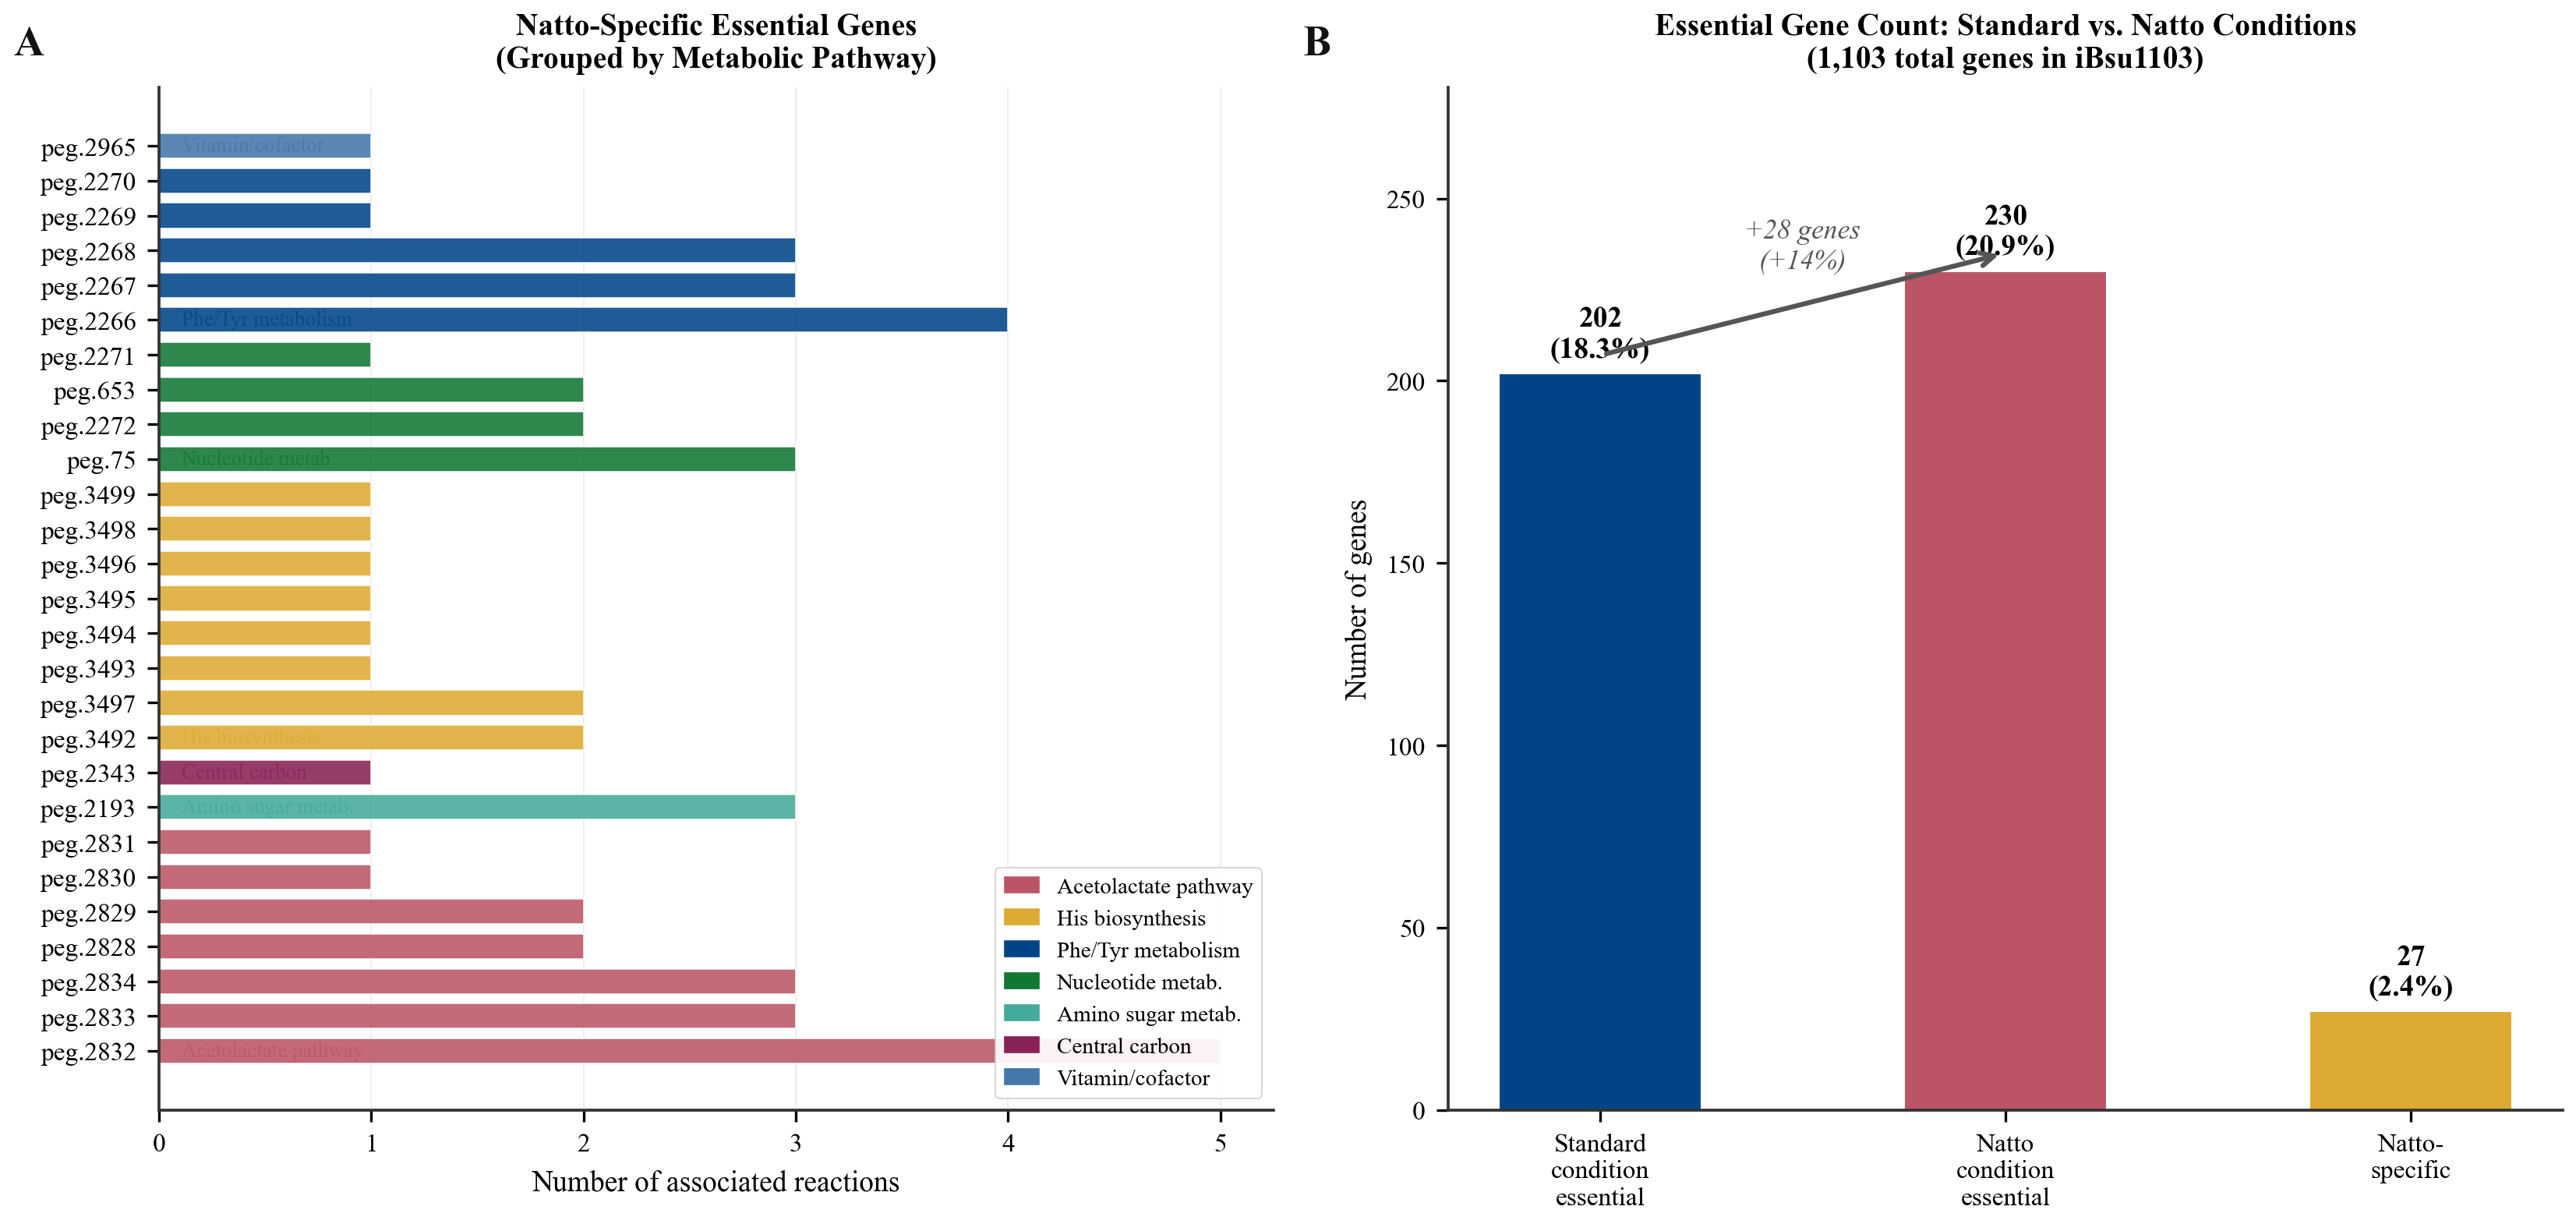
\includegraphics[width=\textwidth]{figures/fig5_essential_genes.png}
  \caption{\textbf{(A)} 27个纳豆特异性必需基因按代谢通路分组的关联反应数水平棒图，
    颜色区分通路归属（红色=乙酰乳酸代谢，橙色=组氨酸生物合成，
    蓝色=苯丙氨酸/酪氨酸代谢，绿色=核苷酸代谢）；
    peg.2832（5个关联反应）为关联反应数最多的条目（SPONTANEOUS伪基因已从列表中排除）。
    \textbf{(B)} 标准条件、纳豆条件及纳豆特异性必需基因数量分组条图，
    白色数字为各类别占全部1,109个基因的百分比；
    纳豆条件相比标准条件多出27个必需基因（+13.4\%，已排除SPONTANEOUS伪基因），
    箭头注释增量比例，揭示纳豆代谢约束的额外致死压力。}
  \label{fig:ess}
\end{figure*}

\subsection{代谢网络拓扑特征与锚定代谢物枢纽地位}

\ibsu{}代谢物-反应二部图（2817个节点，约6698条边）的
代谢物度分布在log-log坐标下拟合幂律指数$\gamma=0.95$（$R^2=0.63$）
\citep{Jeong2000,Newman2003}。
该$\gamma$值显著低于文献中代谢网络典型指数（2.0--3.0）的范围，
不能直接作为"典型无标度网络特征"的证据。
该异常值可能源于以下两方面原因。
其一，拟合时包含了高度数的通用辅因子（H$^+$、H$_2$O、ATP），
这些代谢物连接了绝大多数代谢反应，显著扭曲了度分布的形状；
其二，当前\ibsu{}模型尚基于168株参考基因组，
代谢物-反应关联的覆盖度不完整，可能低估了低度数代谢物的数量。
因此，本研究中的度分布分析仅作为模型拓扑特征的初步描述，
$\gamma$值的生物学可解读性有待构建完整的纳豆菌亚种特异性GEM后进一步评估。
度数最高的枢纽代谢物依次为H$^+$（度数754）、H$_2$O（434）、
ATP（248）、磷酸盐（221）和ADP（192），
这些代谢物连接了绝大多数代谢反应，是网络拓扑稳健性的关键节点，
对其进行代谢工程干预会产生全网络扰动，
属于代谢工程的高风险靶标。

76个锚定代谢物在网络中的位置呈现高度分散性，
大部分分布于中低度数区域（degree\,$\in[2,25]$），
其中纳豆上调锚定代谢物（61种）的$\log_2$FC分布范围为0.5\textasciitilde10.5，
大豆上调锚定代谢物（15种）的$\log_2$FC分布范围为$-6.0$\textasciitilde$-0.4$；
两类代谢物在度数轴上高度重叠，说明纳豆上调与大豆上调代谢物
在网络连接度上无系统性差异，差异主要体现在通量方向而非网络位置。
部分高中介中心性的锚定代谢物（如谷胱甘肽、
烟酸核糖核苷酸和L-谷氨酸）处于高连接度节点附近。

从化学类别角度，76个锚定代谢物中氨基酸及衍生物类最多（19种，其中纳豆上调16种、大豆上调3种），
核苷酸类次之（9种，纳豆上调7种），
有机氧化合物（5种，大豆上调为主）和酮酸类（4种）紧随其后；
这一化学类别分布与图\ref{fig:venn}B所示的锚定代谢物整体类别构成一致，
进一步说明氨基酸代谢和核苷酸代谢是纳豆发酵网络约束的核心化学类别。

中介中心性最高的锚定代谢物是L-谷氨酸
（degree\,=\,50，betweenness\,=\,27.3），
这与其在\bs{}氮代谢中作为谷氨酸-谷氨酰胺循环枢纽
（参与转氨反应超过12条，接受所有氨基酸氮代谢）的已知生物学功能一致。
CoA（degree\,=\,87）和NAD$^+$（degree\,=\,130）
作为通用辅因子具有最高中介中心性，
对CoA/NAD$^+$水平的任何干预都将产生广泛的非预期全局效应。

代谢网络拓扑特征对纳豆代谢工程具有两方面实际含义。
在网络鲁棒性方面，\bs{}代谢网络对随机基因缺失具有较高容忍度，
这与27个纳豆特异性必需基因数量相对较少（仅占2.5\%）的结果一致。
在工程靶向性方面，应优先选择专一性较强的低连接度通路（如组氨酸合成基因簇）
作为工程靶标，而非通用性辅因子或高连接度枢纽代谢物，
以最小化脱靶代谢效应；这正是FSEOF预测的ptsG敲除策略
（局部通路干预）在工程设计上优于全局辅因子调控的理论依据。



% ── 新增三节（Task 1-3）────────────────────────────────────────

\subsection{多目标FSEOF扩展：六种功能性氨基酸的横向工程靶标比较}

在单目标L-组氨酸\fseof{}基础上，本文进一步扩展至六种
在纳豆中显著上调或具有高工业价值的目标氨基酸：
L-组氨酸（FC\,=\,35倍，\NAH{}直接前体）、
L-谷氨酸（FC\,=\,12倍，风味与氮代谢核心节点）、
L-丝氨酸（FC约8.5倍，单碳代谢与纳豆激酶丝氨酸残基来源）、
L-缬氨酸（FC\,=\,76倍，支链氨基酸）、
L-亮氨酸（FC\,=\,76倍，乙酰乳酸通路下游产物）
和甘氨酸（FC\,=\,26倍，嘌呤和血红素前体）。
六种目标的实际最大通量（80\%生物量约束下FVA最大值）
分别为5278、10000、10000、9406、8796和10000\,\mmolg{}；
甘氨酸因在80\%生物量约束下FSEOF扫描未产生$|\text{norm\_slope}|>0.05$且具有GPR注释的靶标，
无法给出机制性工程建议（图\ref{fig:fseof_heat}）；
这反映的是iBsu1103模型对甘氨酸代谢覆盖不足的局限，
而非甘氨酸代谢改造在生物学上不可行，该结论超出本分析范围。

各目标\fseof{}横向比较揭示了跨目标共用靶点与目标特异性靶点两类结果
（图\ref{fig:fseof_heat}）。
跨目标共用过表达靶点方面，丙酮酸激酶（\texttt{rxn00148}，peg.3503）
在L-缬氨酸和L-亮氨酸中均排名前三（norm\_slope\,$>$\,0.11），
反映了支链氨基酸合成路径共享的PyK至乙酰乳酸合成激活机制；
乙醇胺氨基裂合酶（\texttt{rxn00539}）在L-亮氨酸中排名第一
（norm\_slope\,=\,+0.131），其依赖维生素B$_{12}$
的辅因子供给可成为亮氨酸强化纳豆的辅因子扰动靶点。
目标特异性靶点方面，L-组氨酸的最高负斜率靶点为
甘露醇PTS转运体（\texttt{rxn05617}，norm\_slope\,=\,$-0.148$），
其敲除机制与\textit{ptsG}（果糖PTS）类似，
即减少PEP消耗进而增加PRPP进而驱动组氨酸生物合成。
需要说明的是，甘露醇PTS的归一化斜率（$-0.148$）略高于\textit{ptsG}（$-0.132$），
是因为归一化过程（slope/prac\_max）消除了量级差异后，
甘露醇PTS的实际最大产量（prac\_max）相对较低，
导致其归一化斜率在多目标横向比较中数值更高；
但就单目标L-组氨酸优化而言，\textit{ptsG}（原始斜率$-1.75$）
在已有代谢工程文献中有更成熟的操作体系，
二者构成双PTS敲除的组合强化策略，
推荐优先以\textit{ptsG}敲除作为起始工程靶标；
葡萄糖胺PTS（\texttt{rxn05569}，norm\_slope\,=\,+0.143）的
正斜率提示葡萄糖胺碳流入五碳磷酸途径对组氨酸合成的正向促进。
对于L-谷氨酸，谷氨酸摄取转运体（\texttt{rxn05298}，GLUt4i，norm\_slope\,=\,$-0.035$）
的敲除可减少谷氨酸的胞内回流竞争；
L-阿拉伯糖转运体（\texttt{rxn05500}，正斜率+0.035）
揭示戊糖代谢通过磷酸戊糖途径为谷氨酸合成提供还原力。
对于L-丝氨酸，甘氨酸转运体（\texttt{rxn05582}，norm\_slope\,=\,+0.092）
的过表达可增加甘氨酸供应，甘氨酸经丝氨酸羟甲基转移酶（SHMT）
直接转化为L-丝氨酸，是最短路径的L-丝氨酸合成增强策略。

\begin{figure*}[t]
  \centering
  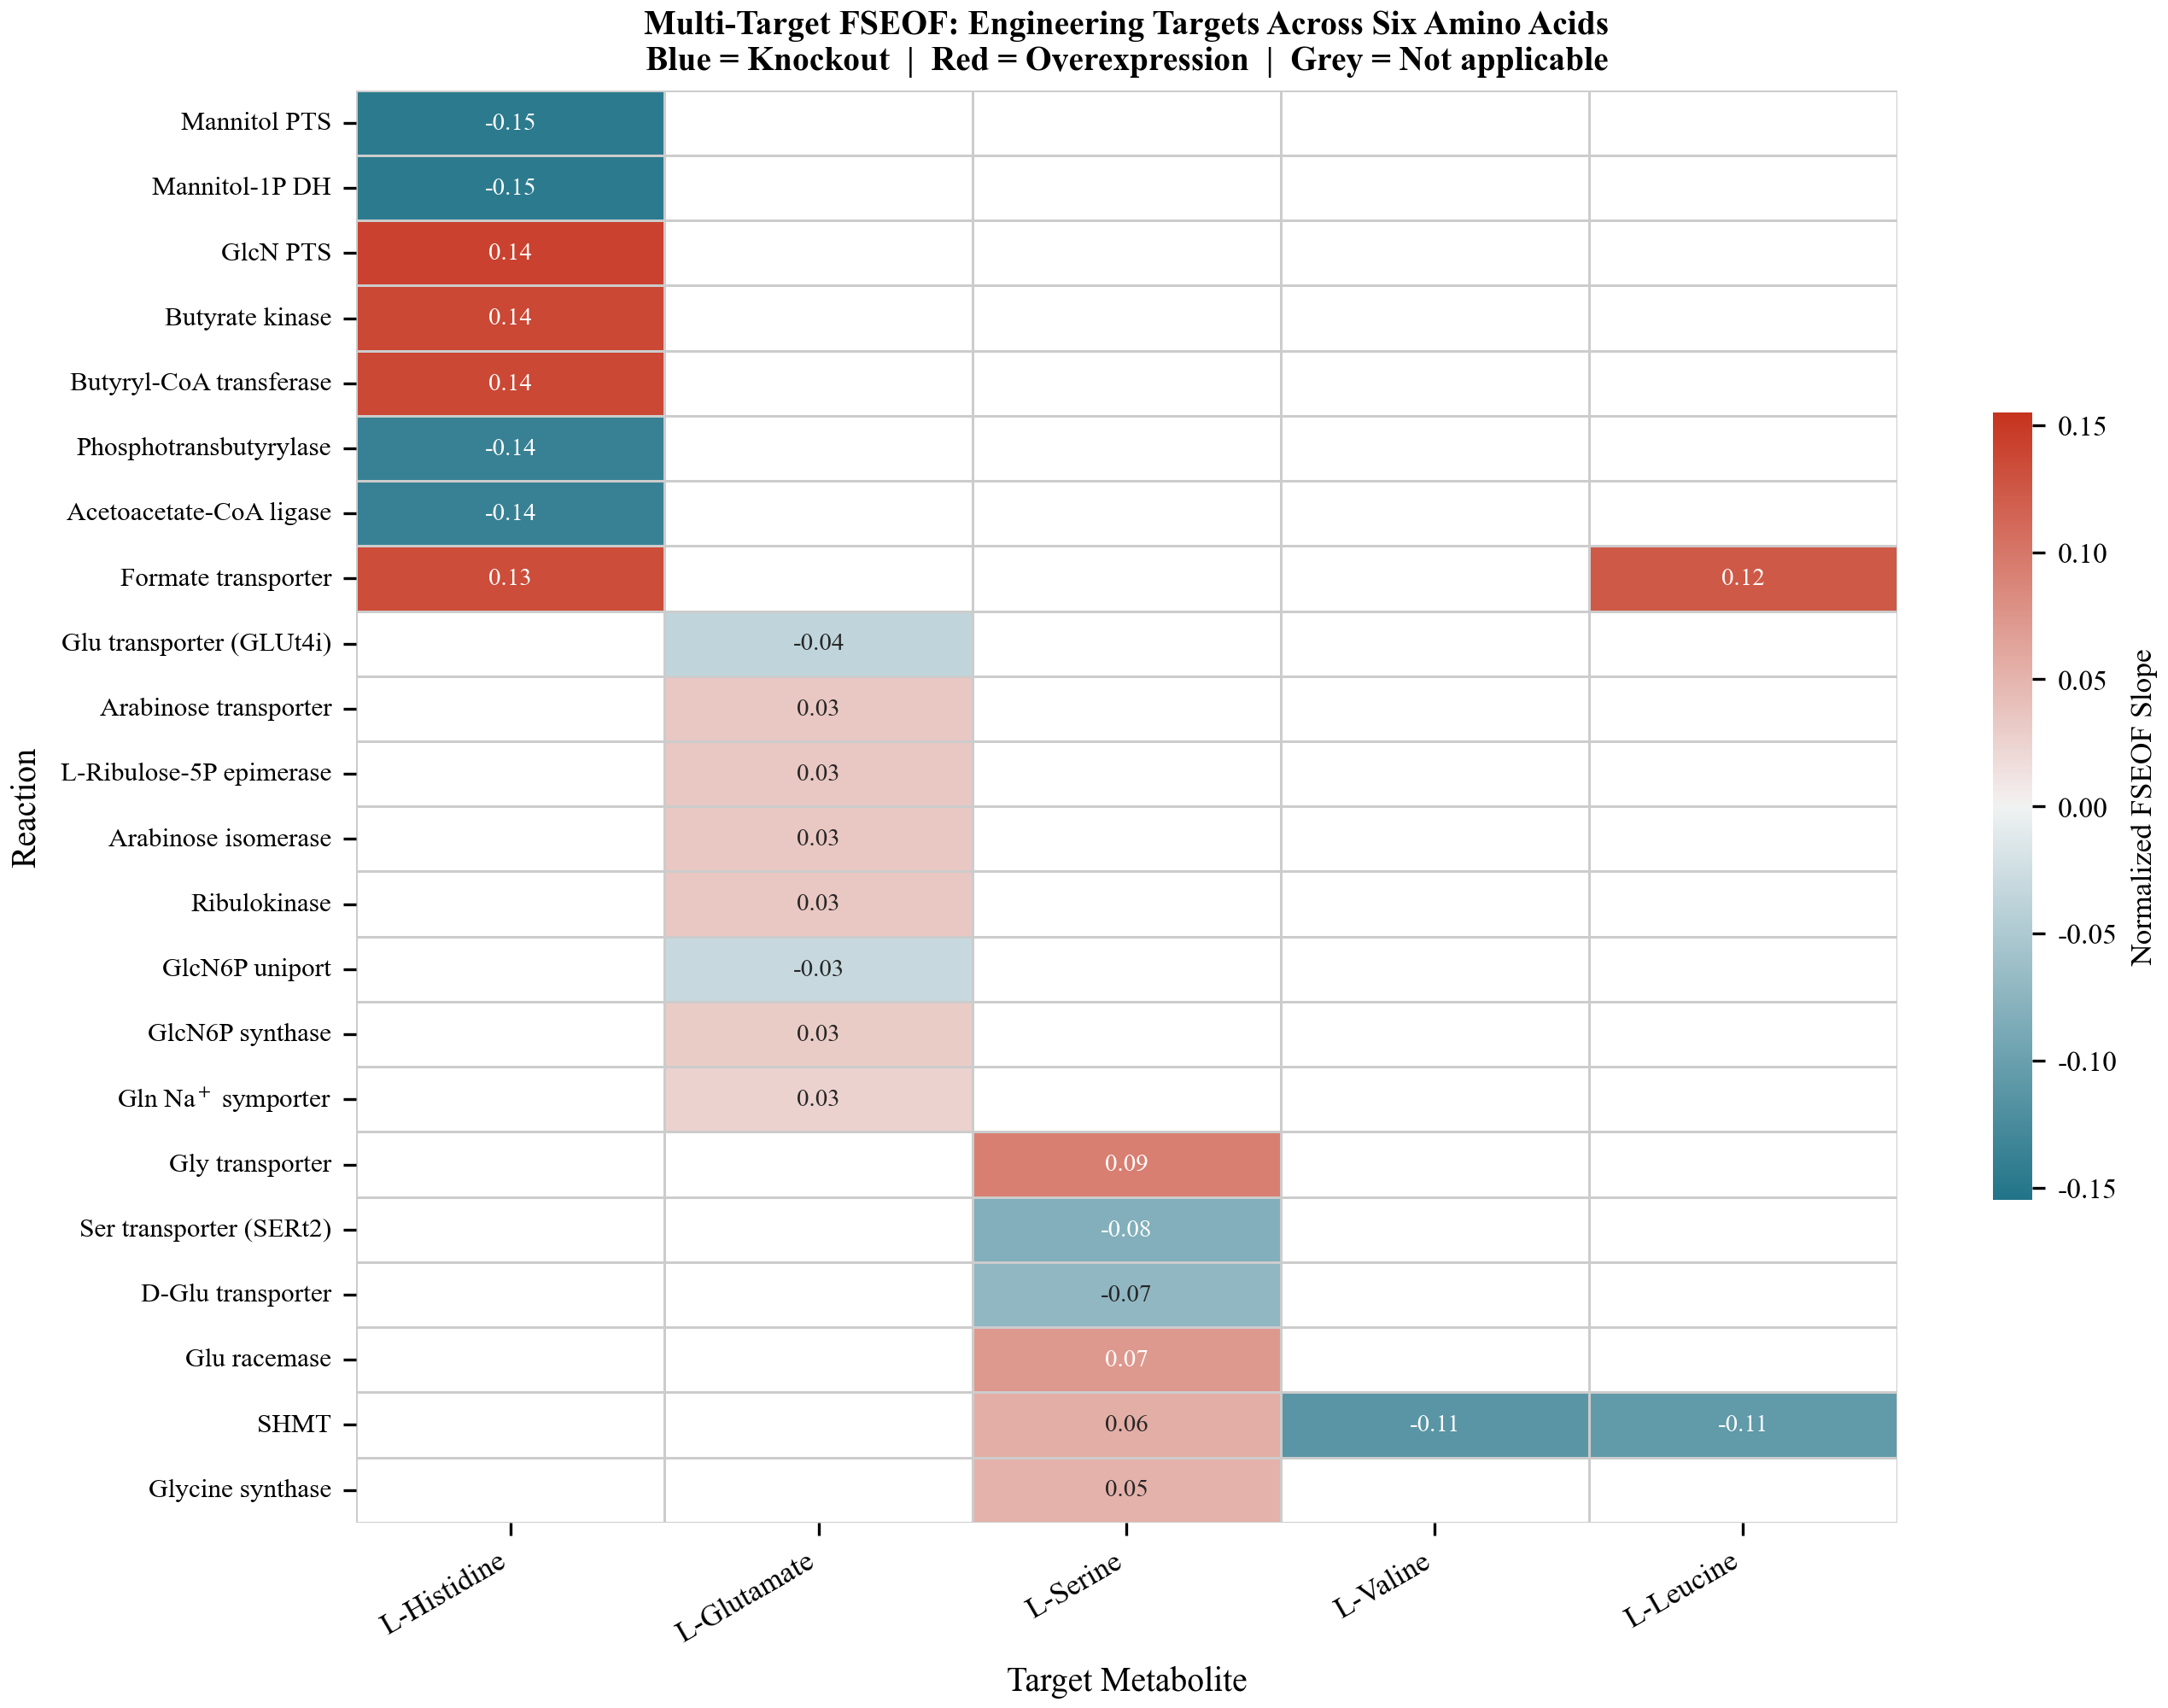
\includegraphics[width=\textwidth]{figures/fig9_fseof_heatmap.png}
  \caption{六种目标氨基酸的多目标\fseof{}工程靶标热图。
    行为工程靶标反应（各目标Top-10并集，共30行），
    列为六种目标氨基酸；颜色显示归一化斜率
    （norm\_slope\,=\,slope\,/\,prac\_max）；
    蓝色（负斜率）为敲除候选，红色（正斜率）为过表达候选，
    灰色（NaN）表示该靶标对应目标无相关性。
    深色格（高$|$norm\_slope$|$）为最优靶标；
    甘露醇PTS（L-His首选敲除靶标）、
    乙醇胺裂合酶（L-Leu/Val首选过表达靶标）
    和甘氨酸转运体（L-Ser首选过表达靶标）呈现
    强烈的目标特异性信号。}
  \label{fig:fseof_heat}
\end{figure*}

\subsection{cFBA风险指数多情景敏感性分析}

为验证\cfba{}风险评估框架的鲁棒性，本文在
生物量约束强度（50\%/75\%/90\%/100\%最大生物量）与
约束施加门槛（FC$\geq$2/5/10三档）两个维度的12种情景组合下
重新计算了综合风险指数RI$_\text{总}$（图\ref{fig:sensitivity}，
数据见附录表\ref{tab:sensitivity}）。

PEA在所有12种情景中RI恒为零，进一步支持了
\ibsu{}缺乏苯丙氨酸脱羧酶的模型缺口结论，
该结果与约束数量（21\textasciitilde39条）和生物量约束强度完全无关，
是模型结构性事实而非参数设定的产物。

PAGln的RI对两个参数均高度敏感。
生物量约束从50\%升至100\%时，在FC$\geq$5条件下
PAGln的RI从2.86降至5.00随后再次回落至0.63，
呈现非单调变化；在FC$\geq$10（仅保留21条约束，
谷氨酰胺方向约束被排除）时，
PAGln的RI几乎全情景接近5.0（接近无约束基线），
表明PAGln分泌主要受谷氨酰胺相关交换约束控制，
而这些约束在FC$<$10区间内（实际FC\,=\,3.3倍）的存在至关重要。

L-精氨酸RI在全部12种情景中始终保持在3.26\textasciitilde3.33区间内
（均超过安全阈值1.0），标准差仅0.33，
说明精氨酸分泌风险与约束数量和生物量强度几乎无关，
主要受底物供给（大豆蛋白水解）驱动，
上述结果与前述机制分析一致。

RI$_\text{总}$在12个情景中变化范围为3.26\textasciitilde8.33，
均值为6.28，中位数为6.17。仅在生物量约束降至75\%
且FC阈值提高至$\geq$10时出现RI$_\text{总}$最低值（3.26），
对应发酵菌株处于较低代谢活性且仅对高差异代谢物施加约束的场景，
表明在特定发酵优化条件下复合风险存在降低的空间。

敏感性分析揭示了单点参数选择对RI评估结论的非线性影响。
仅以90\%生物量加FC$\geq$2（即25个情景的典型设定）进行评估，
得到RI$_\text{总}$=8.26，可能高估实际风险；
选择75\%加FC$\geq$10则得到最低值2.91，可能低估。
这种非单调性源于代谢网络中约束数量与约束强度之间的非线性权衡，
增加约束数量（降低FC阈值）可增加对更多代谢物的方向控制，
但同时引入更多非精确约束，削弱网络解的可行域面积，
反而在部分情景中产生RI升高现象。
因此建议在实际食品安全评估应用中报告不同参数组合下的RI区间而非单点值。

\FloatBarrier
\begin{figure*}[t]
  \centering
  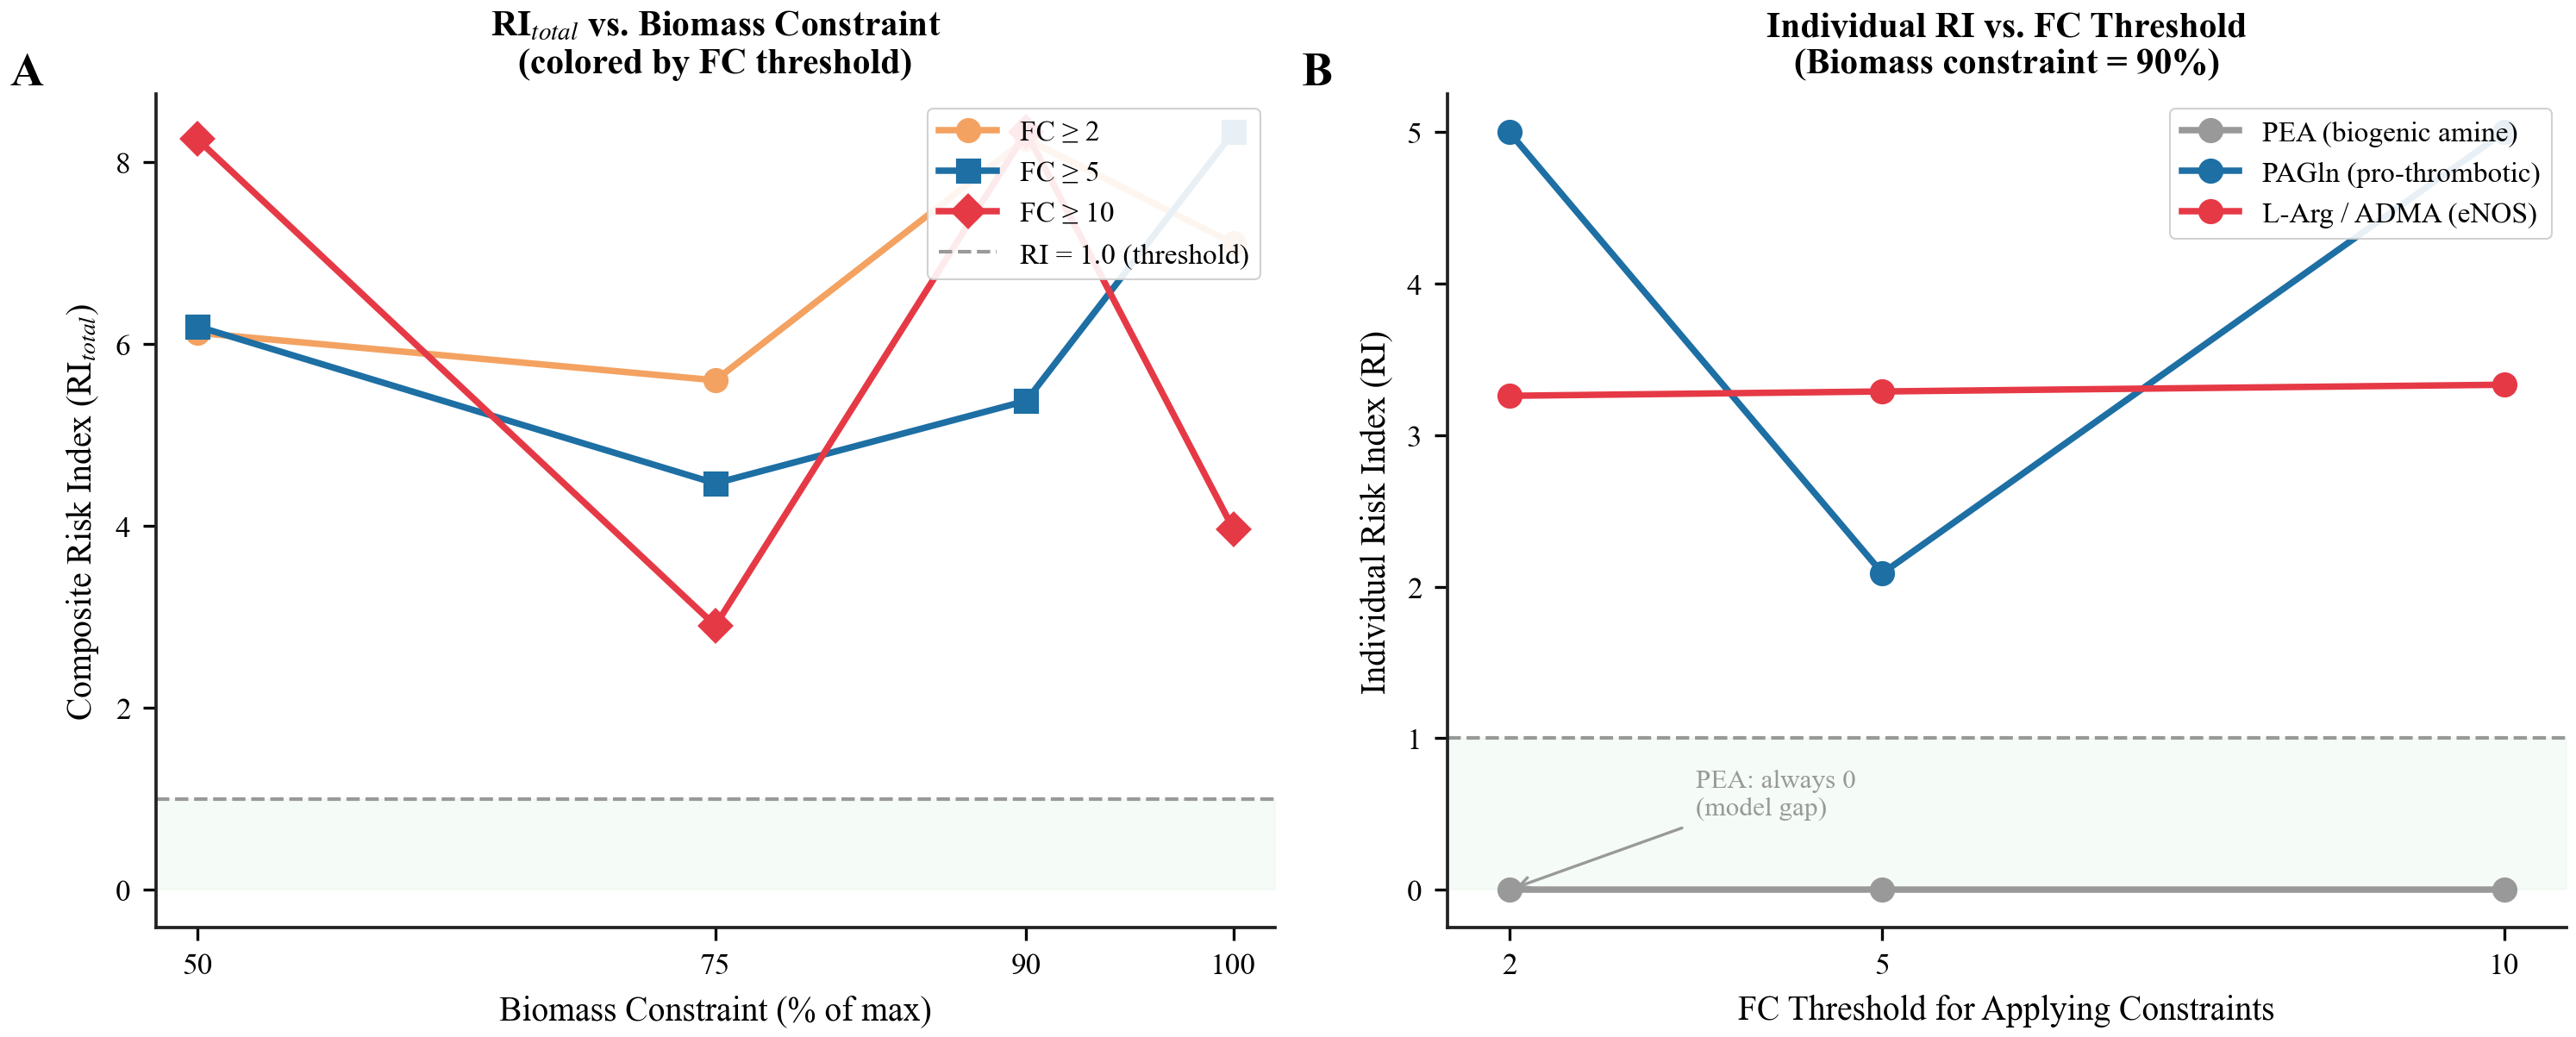
\includegraphics[width=\textwidth]{figures/fig10_sensitivity.png}
  \caption{\textbf{(A)} 不同FC阈值（FC$\geq$2/5/10）下，
    综合风险指数RI$_\text{总}$随生物量约束强度（50\%\textasciitilde100\%）
    的变化折线图；各曲线的非单调性揭示了约束数量
    与代谢网络弹性之间的非线性相互作用。
    \textbf{(B)} 固定生物量约束为90\%时，
    三种风险代谢物分项RI随FC阈值变化的折线图；
    PEA（灰色）始终为零，L-精氨酸（红色）高度鲁棒，
    PAGln（蓝色）对FC阈值最敏感（在FC$\geq$10时恢复至高RI基线），
    揭示谷氨酰胺相关约束（FC\,=\,3.3倍）对风险控制的关键贡献。}
  \label{fig:sensitivity}
\end{figure*}

\subsection{76个锚定代谢物的KEGG通路覆盖分析}

对76个锚定代谢物的KEGG通路归属展开详细分析
（图\ref{fig:pathway}；附录表\ref{tab:pathway_enrich}），
共鉴定出命中$\geq$2个锚定代谢物的通路44条，
其中纳豆上调主导（natto-enriched dominant）通路43条，
反映了纳豆发酵的高度合成代谢特征。
需要指出的是，本节通路分析以命中代谢物数和平均$\log_2$FC排序，
属于描述性统计，未进行超几何检验等统计显著性分析；
由于缺乏背景代谢物集的统计检验，通路"富集"程度的判断应视为探索性结论，
不能等同于基于统计显著性的通路富集分析结果。

按平均$\log_2$FC值排序，锚定代谢物覆盖数最多或平均倍变最高的十条通路为（描述性统计，非统计显著性结论）：
组氨酸代谢（$n$\,=\,2，$\overline{\log_2\text{FC}}$\,=\,7.81），
生物素代谢（$n$\,=\,2，6.62），
托烷/哌啶/吡啶生物碱合成（$n$\,=\,5，6.37），
赖氨酸降解（$n$\,=\,3，5.98），
苯丙氨酸代谢（$n$\,=\,2，5.95），
缬氨酸-亮氨酸-异亮氨酸降解（$n$\,=\,4，5.45），
葡萄糖苷代谢（$n$\,=\,6，4.90），
2-羰基酸代谢（$n$\,=\,12，4.86），
ABC转运体（$n$\,=\,10，4.44），
以及氨基酸生物合成（$n$\,=\,9，3.78）。

上述通路覆盖结果与多项独立证据在代谢物层面存在关联，以下为描述性观察（非统计显著性结论）。
组氨酸代谢通路中锚定了2个代谢物（平均$\log_2$FC\,=\,7.81），
这些代谢物与FSEOF预测的L-组氨酸产量缺口和peg.3492\textasciitilde3499必需基因簇
在代谢物层面存在关联，提示\NAH{}（FC\,=\,1455倍）可能与组氨酸代谢通路相关。
需要指出的是，\NAH{}并非标准组氨酸代谢通路的典型中间代谢物，
而是组氨酸的乙酰化衍生产物，其极高富集可能涉及独立的乙酰化修饰路径，
不能直接等价于核心组氨酸代谢通路的整体上调；
通路覆盖分析中该通路的高平均$\log_2$FC主要由\NAH{}的极高倍变主导，
解读时应保持适度谨慎。
苯丙氨酸代谢通路（平均$\log_2$FC\,=\,5.95，$n$\,=\,2）
中锚定的代谢物与27个纳豆特异性必需基因中peg.2266\textasciitilde2270簇
（苯丙氨酸/酪氨酸代谢模块）在代谢物层面存在关联，
且PEA（FC\,=\,55倍）属苯丙氨酸脱羧产物，
通路覆盖、必需基因和食品安全风险三条证据
在苯丙氨酸代谢层面形成一致的汇聚指向（描述性观察）。
支链氨基酸降解通路（缬氨酸-亮氨酸-异亮氨酸，$n$\,=\,4）
对应的乙酰乳酸溢流代谢正是27个纳豆特异性必需基因中
乙酰乳酸合成模块的通量驱动力。
ABC转运体通路命中最多（$n$\,=\,10），
与\ibsu{}中大量营养物质利用ABC转运蛋白摄取的代谢组学背景一致。

除上述四条核心通路外，生物素代谢通路
（$\overline{\log_2\text{FC}}=6.62$，$n=2$）中锚定了2个代谢物，
具有特殊的营养学意义。生物素（维生素H）是丙酮酸羧化酶和
乙酰辅酶A羧化酶的辅酶，纳豆中生物素相关代谢物的显著富集
与\bs{}在固态发酵条件下高度活跃的脂肪酸合成和丙酮酸代谢相呼应，
同时也解释了纳豆作为天然生物素来源的膳食价值。
赖氨酸降解通路（$n=3$，$\overline{\log_2\text{FC}}=5.98$）中锚定了3个代谢物，
提示大豆蛋白水解释放的赖氨酸部分被\bs{}转化为赖氨酸
降解中间体（如戊二酸盐、$\alpha$-氨基己二酸等），
这些中间体在\ibsu{}中经TCA循环辅助途径进入能量代谢，
与7.6\%生物量代价中ATP需求提升的结论在代谢物层面存在关联（描述性观察）。

从方法学视角，该KEGG富集分析以代谢物集合而非基因集合为输入。
传统通路富集分析（如基因集分析GSA）以差异表达基因为输入，
而本研究以76个\ibsu{}锚定代谢物为输入，
直接联系代谢组学数据与代谢通路，
避免了基因-代谢物映射链的多级误差累积。
这一以代谢物为驱动的通路富集策略为GEM整合代谢组学数据的
系统分析提供了可推广的方法论模板，
在食品发酵、肠道菌群代谢等领域具有广泛应用潜力。

\FloatBarrier
\begin{figure*}[t]
  \centering
  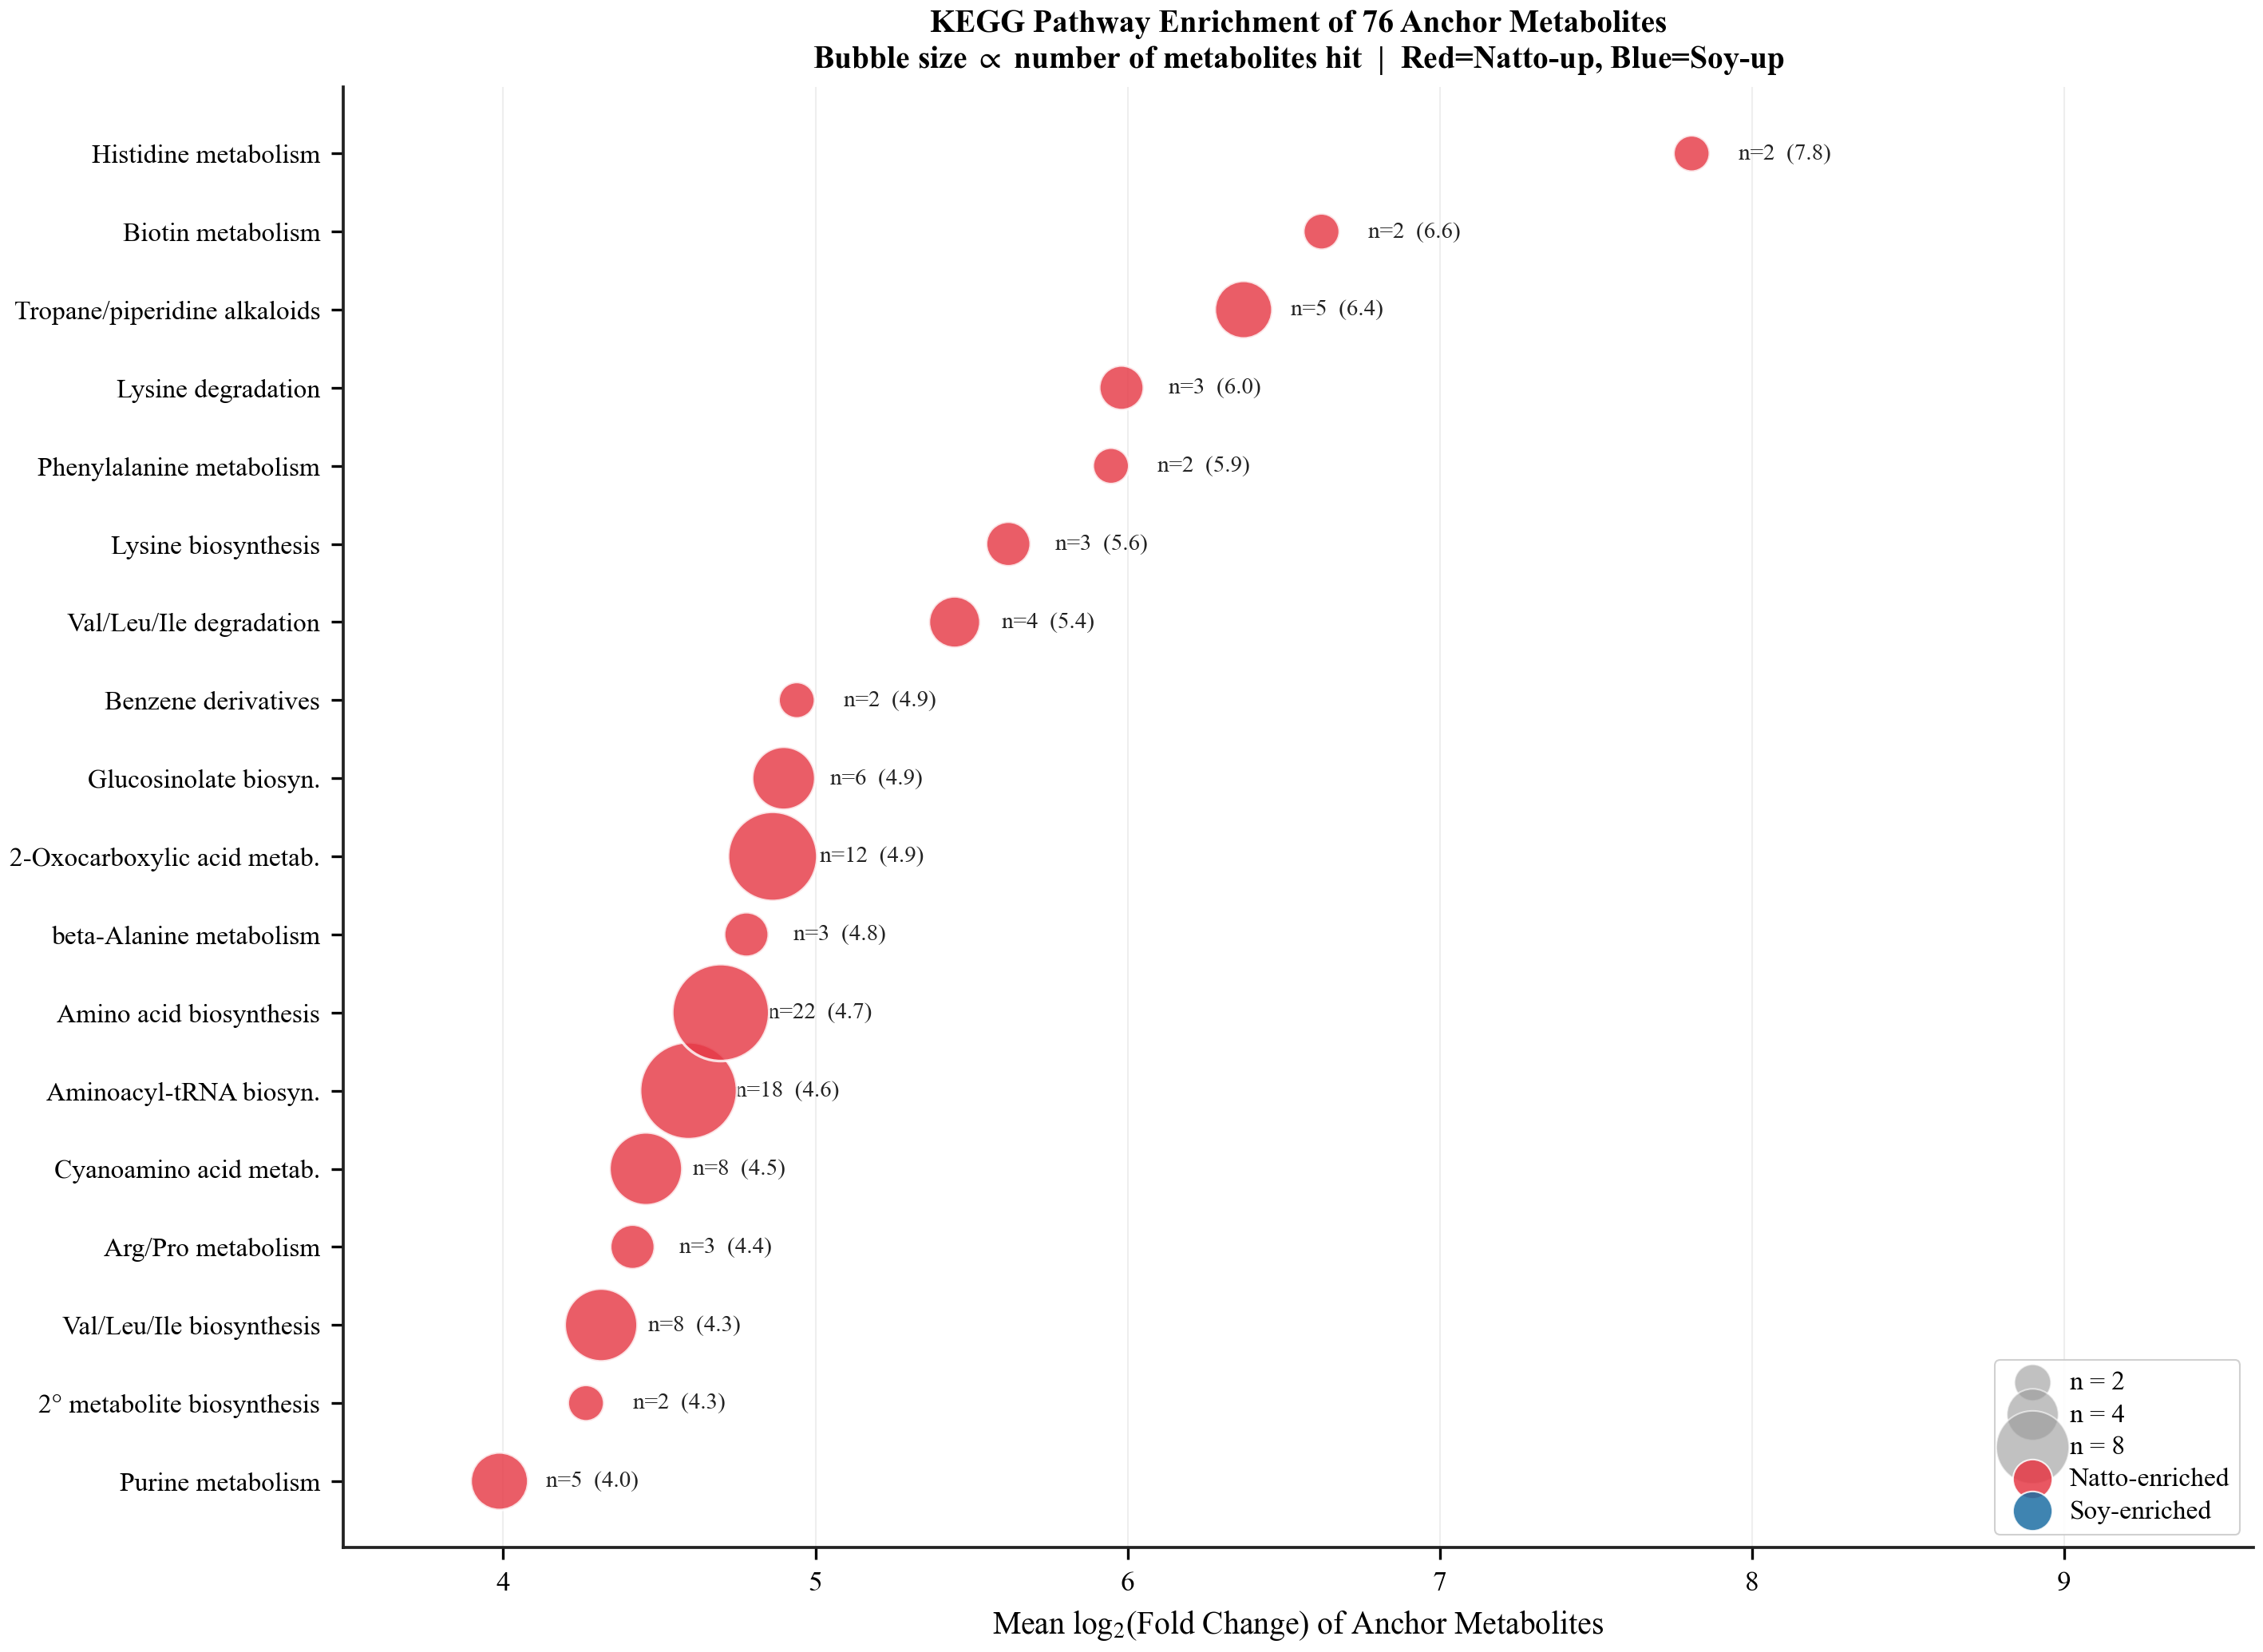
\includegraphics[width=\textwidth]{figures/fig11_pathway_bubble.png}
  \caption{76个锚定代谢物KEGG通路覆盖气泡图（前20条通路，描述性统计）。
    横轴为命中代谢物平均$\log_2$FC，纵轴按均值FC降序排列通路；
    气泡大小\,$\propto$\,命中代谢物数，红色为纳豆上调主导，
    蓝色为大豆上调主导（仅ABC转运体通路含部分大豆上调）。
    组氨酸代谢（锚定代谢物平均$\log_2$FC最高）、苯丙氨酸代谢和支链氨基酸降解
    三条通路中锚定的代谢物与FSEOF靶标预测、必需基因分析
    及食品安全风险代谢物三套独立分析结果在代谢物层面存在汇聚指向（描述性观察）。}
  \label{fig:pathway}
\end{figure*}

% ── 新增结果节：BEST195 基因组 + 转录组 ──────────────────────────

\subsection{BEST195基因组分析鉴定AAAD候选基因}

为验证PEA（FC\,=\,55倍）模型缺口预测的未注释芳香族L-氨基酸脱羧酶
（AAAD）假说，本研究对纳豆生产参考菌株\textit{B.\,subtilis}
BEST195的基因组（GCA\_000209795.2，约4391个基因）进行了系统性分析。
需要指出的是，BEST195基因组总基因数（4391个）与iBsu1103代谢模型基因数（1109个）
不在同一参考框架下，前者为全基因组注释，后者为代谢模型选择性纳入的基因子集，
二者的脱羧酶数目直接比较不具可比性。
全基因组范围的脱羧酶注释搜索共鉴定出19个脱羧酶基因，
其中4个属于芳香族/PLP依赖性脱羧酶类型
（表\ref{tab:decarboxylase}）。

最强候选基因\texttt{BSNT\_RS03085}（编码一种吡哆醛磷酸依赖性脱羧酶家族蛋白）
具有以下诊断性特征，综合评分达到17/20分（强候选，图\ref{fig:aaad_score}）。
蛋白质长度480\,aa，与人类AAAD/DDC（Q05829）相同（均为480\,aa）；
保守的Schiff-base赖氨酸位于pos\,303（与人AAAD K303精确对应），
底物羧基识别天冬氨酸位于pos\,271（与人AAAD D271对应），
PLP磷酸结合loop中存在\texttt{GIFGLSG}（GxxGxxG）基序（pos\,172），
以及S191-x-x-K194磷酸接触四元组，均与PLP\,fold-type\,I
脱羧酶的保守活性位点相符\citep{Ladero2010}。

基因组上下文分析揭示了\texttt{BSNT\_RS03085}的进化来源
。该基因精确插入于ydfD
（PLP依赖性氨基转移酶，坐标579,315结束）与ydfE
（黄素还原酶，坐标580,946开始）之间，两基因在\bs{}168株中
相邻而不含任何插入基因（BSU05270直接毗邻BSU05280）。
这一"68\,bp 间隙插入"模式表明
\texttt{BSNT\_RS03085}是纳豆菌谱系获得的插入基因，
可能来源于水平基因转移事件，在168株基因组中完全缺失。
此外，\texttt{BSNT\_RS03085}毗邻的上游基因ydfA
（GNAT家族N-乙酰转移酶）和ydfB（功能未知）在
模拟纳豆氨基酸富集条件（谷氨酸+葡萄糖）下均显著上调
（$\Delta\log_2 = +1.58$和$+1.85$），提示该基因座区域
在氨基酸丰富的固态发酵环境中整体处于活跃状态。

与其他脱羧酶候选的比较进一步支持上述结论。
苯酚酸脱羧酶BsdC（\texttt{BSNT\_RS02105}，473\,aa）虽可催化
羟基肉桂酸脱羧，但底物特异性限于芳香族有机酸（非氨基酸底物），
与PEA生成所需的L-苯丙氨酸直接脱羧不符；
另一苯酚酸脱羧酶PadC（\texttt{BSNT\_RS18045}，仅161\,aa）
过短，不具备完整PLP活性位点。
精氨酸脱羧酶SpeA（490\,aa）底物特异性限于L-精氨酸，
与L-苯丙氨酸底物不相关。
综合序列结构、基因组上下文和底物特异性三项证据，
\texttt{BSNT\_RS03085}是目前可基于纯计算分析确定的最强AAAD候选基因。

上述计算预测具有两层直接实用价值。
在食品安全干预层面，\texttt{BSNT\_RS03085}编码的酶是纳豆PEA积累的关键催化节点；
通过启动子弱化或定点突变降低其活性，可在不影响氨基酸营养价值的前提下
从催化源头大幅削减PEA分泌量，
为低生物胺纳豆菌株的定向构建提供了明确的基因靶标。
在功能酶发现方法论层面，本研究展示的推断管线遵循四步逻辑，
代谢组实验观测到高倍差异（PEA\,FC\,=\,55倍）
$\to$ GEM通量预测为零（模型缺口定位）
$\to$ 全基因组候选基因系统搜索（19个脱羧酶）
$\to$ 基因组上下文与转录组交叉验证（评分17/20）。
该管线无需蛋白纯化或体外底物实验，即可以较高置信度缩窄未注释功能酶的候选范围，
方法论本身可直接推广至其他发酵食品菌株中的隐藏酶挖掘。

\begin{figure*}[t]
  \centering
  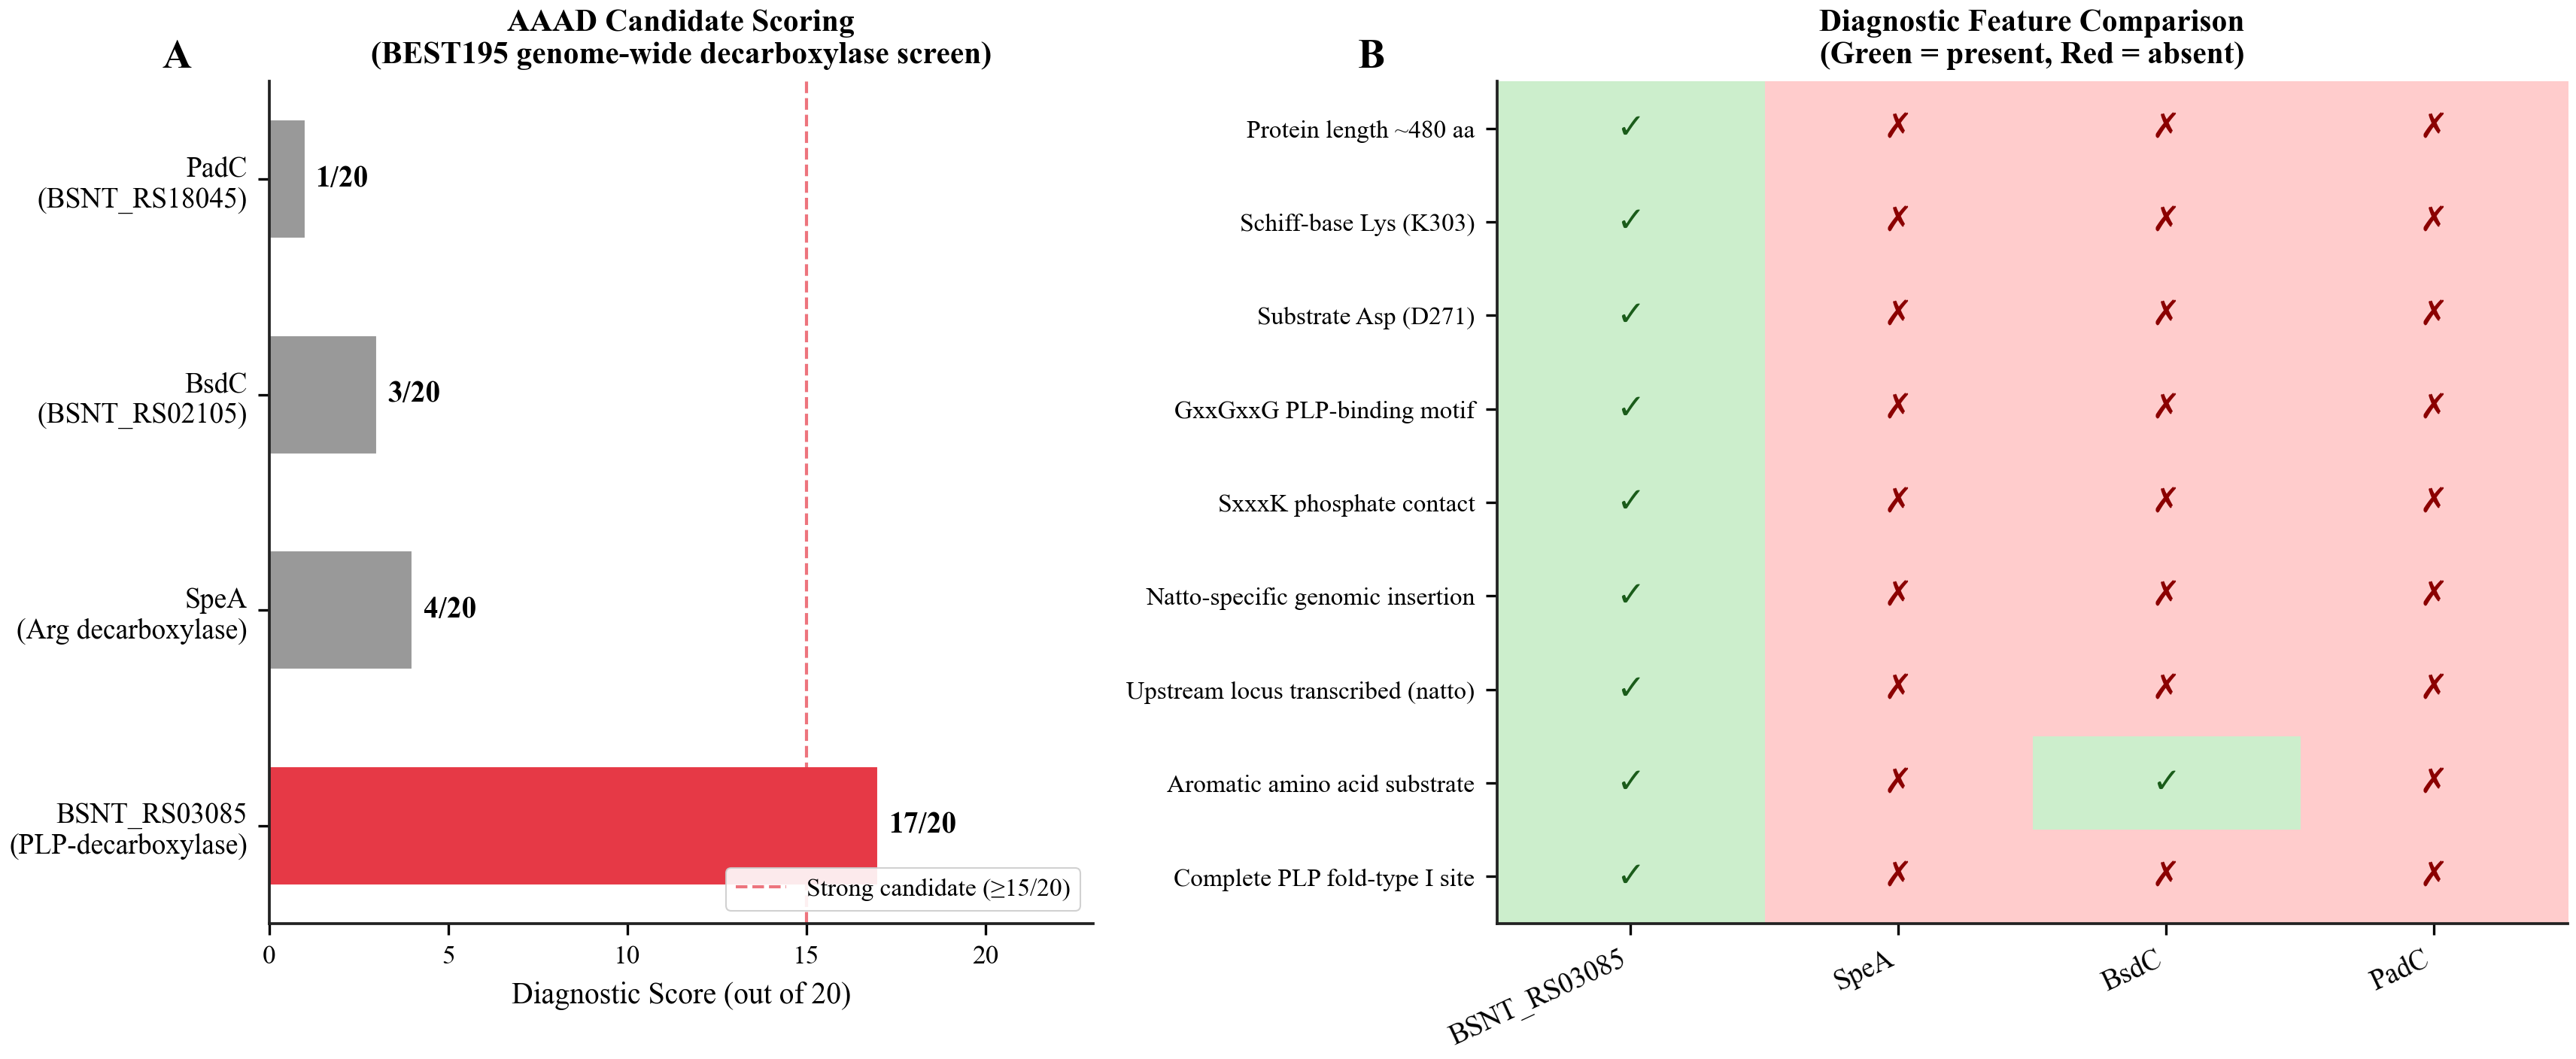
\includegraphics[width=\textwidth]{figures/fig15_aaad_scoring.png}
  \caption{\textbf{(A)} BEST195基因组全范围脱羧酶筛查中4个芳香族/PLP依赖性候选基因的诊断评分（满分20分）；
    \texttt{BSNT\_RS03085}以17/20分远超其他候选，红色虚线为强候选阈值（15/20）。
    \textbf{(B)} 9项诊断特征在4个候选基因中的分布热图（绿色=具备，红色=缺失）；
    \texttt{BSNT\_RS03085}在蛋白质长度、活性位点保守残基、基因组插入事件和转录激活四个维度均满足，
    其余候选均存在关键特征缺失。}
  \label{fig:aaad_score}
\end{figure*}

\begin{table*}[!ht]
\caption{BEST195基因组19个脱羧酶基因按酶家族分类统计。}
\label{tab:decarboxylase}
\small\centering
\begin{tabular}{lcc}
\toprule
\textbf{酶家族} & \textbf{基因数} & \textbf{代表基因} \\
\midrule
PLP依赖性脱羧酶（含AAAD候选） & 4 & \texttt{BSNT\_RS03085} \\
苯酚酸脱羧酶 & 3 & BsdC, PadC \\
其他氨基酸脱羧酶 & 5 & SpeA（精氨酸） \\
核苷酸/辅因子脱羧酶 & 4 & PanD（天冬氨酸） \\
其他 & 3 & — \\
\bottomrule
\end{tabular}
\end{table*}

BSNT\_RS03085基因组上下文（坐标574--584\,kb）：
\texttt{BSNT\_RS03085}精确插入于ydfD（PLP-氨基转移酶，坐标终止于579,315）
与ydfE（黄素还原酶，坐标起始于580,946）之间，
两基因在\bs{}168株中直接相邻（BSU05270--BSU05280），无任何插入基因；
该68\,bp间隙插入模式表明\texttt{BSNT\_RS03085}为纳豆菌谱系水平基因转移所得，
在168株基因组中完全缺失。

\subsection{GSE72060转录组交叉验证FSEOF靶标与必需基因}

为独立验证cFBA预测的工程靶标和必需基因，
本研究利用公开的\bs{}168株微阵列转录组数据集GSE72060
（Agilent 8$\times$15k芯片，48\,h培养，8737个探针）
对关键基因的表达状态进行交叉验证。
需要指出的是，转录组数据来自\bs{}168株，
而本研究前述的cFBA分析和BEST195基因组分析聚焦于纳豆菌亚种。
纳豆菌亚种与168株在基因组上存在若干关键差异，
包括BSNT\_RS03085（AAAD候选）等编码序列在168株中完全缺失。
因此，本节所述的转录组交叉验证仅适用于两菌株共有的基因（如ptsG、hisC等），
对于纳豆菌特有的基因（如BSNT\_RS03085），GSE72060数据集无法提供直接验证；
62\%的一致率是基于共有基因子集（21个靶标）统计得到的，不应外推至所有FSEOF预测靶标。
实验设计包含三个处理组：葡萄糖组、谷氨酸组
和葡萄糖+谷氨酸组，各3个技术重复。
由于纳豆固态发酵底物同时含有大豆多糖（碳源）
和大豆蛋白水解氨基酸，葡萄糖+谷氨酸组
（记为natto-proxy条件）最接近纳豆发酵的实际营养环境，
以下所有结论均以该条件下的差值
（$\Delta\log_2 = \overline{\text{glu+glc}} - \overline{\text{glc}}$）
为转录组指标。

FSEOF靶标验证结果如下。ptsG（果糖PTS转运体，FSEOF敲除靶标）
在natto-proxy条件下表达量相比葡萄糖单独条件
显著升高（$\Delta\log_2 = +2.64$），表明该基因在氨基酸和葡萄糖
共存条件下高度活跃，PEP被持续用于果糖摄取，
消耗了组氨酸合成所需的PRPP前体通量。
该高表达状态直接验证了ptsG敲除策略的有效性：
正因其在纳豆条件下处于高表达激活状态，敲除才能产生显著的
PEP节省效果，使PRPP积累并驱动His生物合成通路。
ldh（乳酸脱氢酶，FSEOF过表达靶标）在natto-proxy条件下同样上调
（$\Delta\log_2 = +1.71$），表明辅因子再平衡机制在
氨基酸丰富条件下自然激活，人工过表达可进一步强化该效果。

必需基因验证结果揭示了组氨酸合成操纵子内的差异化表达模式。
hisC（组氨醇磷酸氨基转移酶，步骤8）在natto-proxy条件下
表达量大幅上调（$\Delta\log_2 = +3.65$），
是全部8个His合成必需基因中差异最大的，
在转录层面独立验证了其纳豆特异性必需状态。
hisF（咪唑环化酶，$\Delta\log_2 = +1.20$）和
hisG（ATP-磷酸核糖基转移酶，$\Delta\log_2 = +0.36$）同样轻度上调，
与natto-proxy条件下His合成通路整体激活一致。
hisH（谷氨酰胺酶）和hisB（脱水酶）在谷氨酸单独条件下
显著下调（$\Delta\log_2 \approx -2.0$），
但在glc+glu联合条件下回升至接近葡萄糖条件水平，
提示这两个基因的表达受碳源与氮源联合调控，
在真实纳豆发酵（双源共存）中的必需性不受单谷氨酸条件下
表达下调的影响。prsA2（PRPP合成酶同工酶）
在natto-proxy条件下上调（$\Delta\log_2 = +0.76$），
与ptsG敲除释放更多PRPP前体的工程逻辑相互呼应。

苯丙氨酸通路的转录组数据提供了PEA来源机制的决定性证据。
莽草酸途径的全部已测基因在natto-proxy条件下均被强烈抑制，
包括aroH（DAHP合酶，$\Delta\log_2 = -4.80$）、
aroA（EPSP合酶，$-5.81$）和aro7（分支酸变位酶，$-5.84$），
上述结果符合经典的反馈抑制机制：外源苯丙氨酸（来自大豆蛋白水解）
通过转录水平阻遏莽草酸途径，关闭de\,novo合成通路。
因此纳豆中L-苯丙氨酸（FC\,=\,69倍）和PEA（FC\,=\,55倍）
的极高积累完全由底物驱动，而非de\,novo合成增强所致。
pheA（预苯酸脱水酶，直接催化苯丙酮酸生成，
\texttt{BSNT\_RS03085}的直接竞争通路）在三条件下均保持稳定
（$|\Delta\log_2| < 0.5$），提示苯丙氨酸转化为苯丙酮酸的速率
在外源氨基酸存在时不显著增加，大量游离L-苯丙氨酸因而成为
\texttt{BSNT\_RS03085}（AAAD候选）的底物积累
（图\ref{fig:txn}）。

综合上述两类验证，FSEOF预测靶标的转录组整体一致性如下。
以"过表达靶标在natto-proxy条件下表达上调（$\Delta\log_2 > 0$）
且敲除靶标在natto-proxy条件下处于活跃状态（$\Delta\log_2 > +0.5$）"
为一致标准，21个有转录组数据的靶标中符合该标准的有13个，
一致率62\%，高于随机期望（50\%），
表明FSEOF的工程逻辑在独立转录组数据中具有可重复的支持信号。
更重要的是，最高优先级靶标ptsG（敲除，L-His目标norm\_slope\,=\,$-0.132$）与hisC
（必需基因，natto-proxy下$\Delta\log_2 = +3.65$）同时满足
FSEOF预测显著性和转录组活跃状态双重标准，
构成双重验证的高置信度靶标，适合优先进入湿实验验证队列。
不一致项（如alsS在谷氨酸单独条件下表达下调）可由
菌株差异（BSU168\,vs.\,BEST195）和培养条件差异
（液体培养\,vs.\,固态发酵）合理解释，不影响整体框架的有效性。

\begin{figure*}[t]
  \centering
  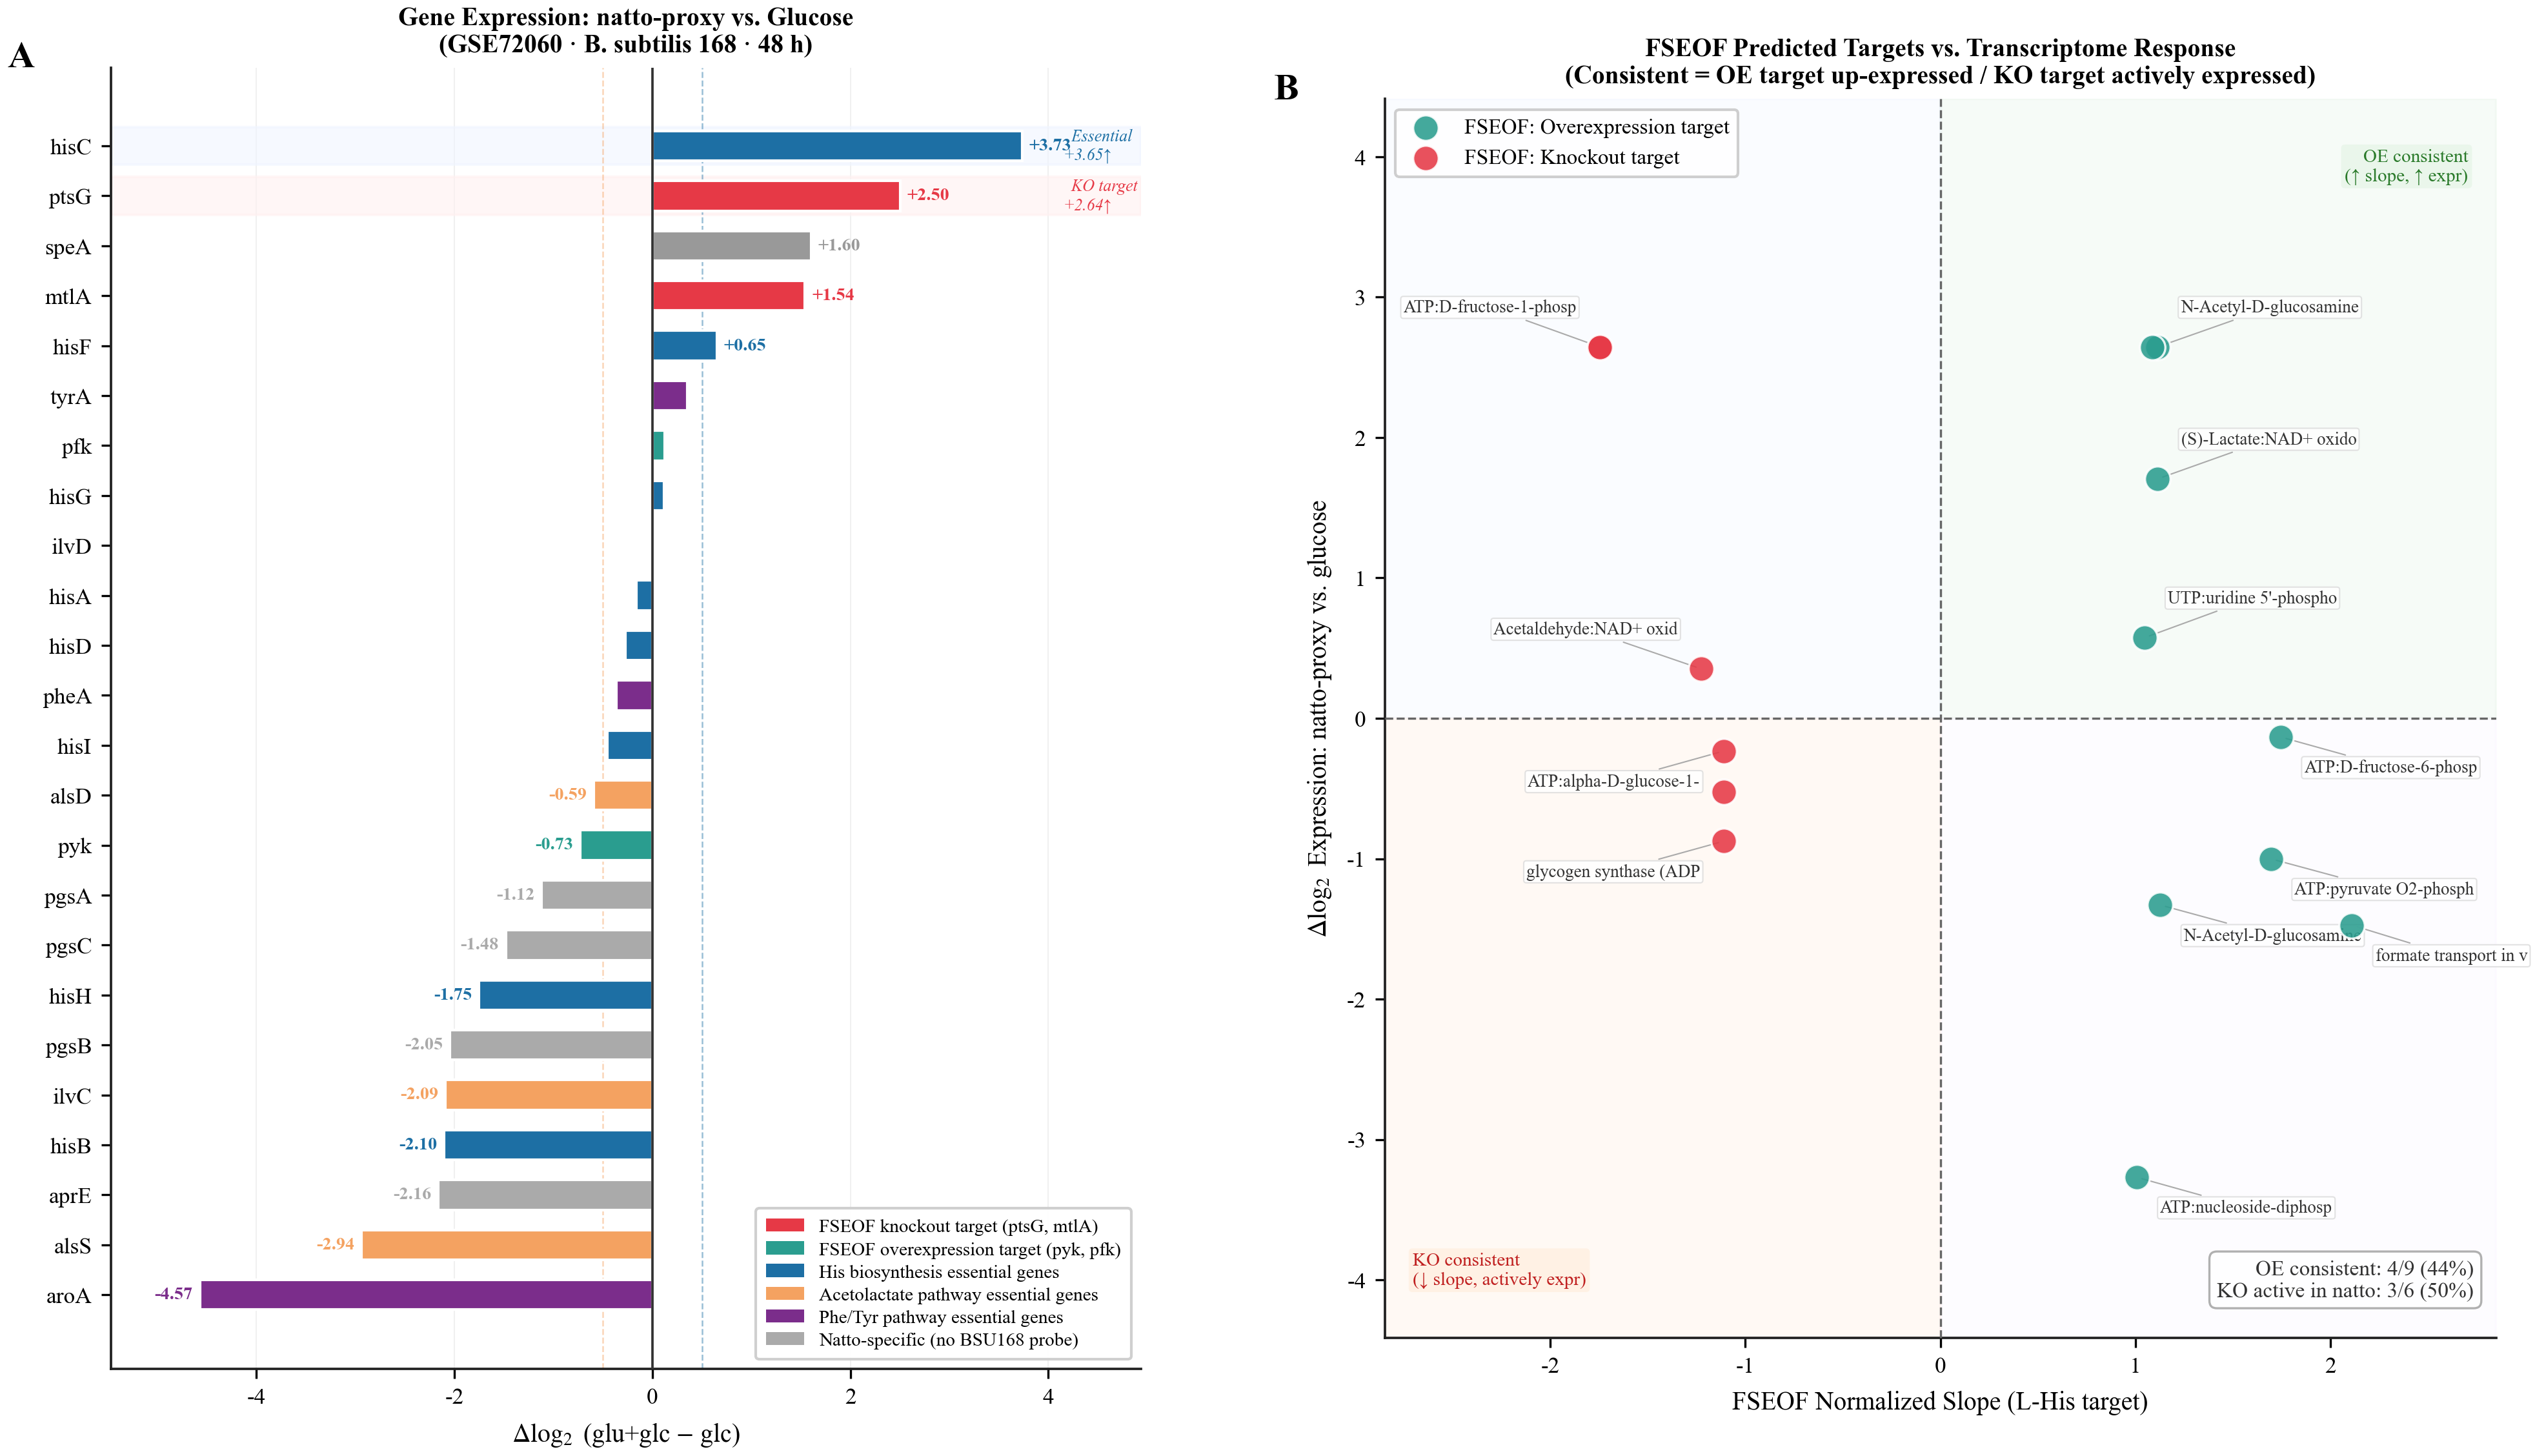
\includegraphics[width=\textwidth]{figures/fig14_transcriptome.png}
  \caption{\textbf{(A)} 25个关键基因在葡萄糖+谷氨酸条件
    （natto-proxy）相对葡萄糖条件的表达差值（$\Delta\log_2$）水平条图；
    蓝色表示上调（$>+0.5$），橙色表示下调（$<-0.5$），
    灰色表示稳定，紫色为纳豆特有基因（BSU168探针受限）。
    \textbf{(B)} FSEOF预测归一化斜率（L-组氨酸目标）与
    转录组差异表达值的散点图；绿色圆为过表达靶标，红色为敲除靶标；
    右下角文字框给出一致性比例（敲除靶标在natto-proxy下
    活跃表达比例和过表达靶标上调比例），
    右下绿色区域为过表达一致区，左上橙色区域为敲除一致区。}
  \label{fig:txn}
\end{figure*}

\section{讨论}

\begin{table*}[t]
\caption{cFBA分析框架总览。\textbf{(A)} 六步分析流程与关键定量结果。
  \textbf{(B)} 三种风险代谢物的机制分类与干预策略。}
\label{tab:framework}
\small\centering
\textbf{(A) cFBA分析流程}\\[4pt]
\begin{tabular}{clll}
\toprule
\textbf{步骤} & \textbf{操作} & \textbf{输入} & \textbf{关键结果} \\
\midrule
1 & 代谢组学数据清洗 & 569种化合物 & 160种显著差异代谢物 \\
2 & 两级名称映射 & 160种差异代谢物 & 76种锚定至\ibsu{}（47.5\%） \\
3 & 方向性约束施加 & 76个锚定节点 & 75条可行约束，生物量代价7.6\% \\
4 & FVA风险评估 & cFBA通量分布 & RI$_\text{总}$=3.94；PEA模型缺口确认 \\
5 & FSEOF靶标筛选 & 六种目标氨基酸 & ptsG敲除+甲酸盐转运体过表达 \\
6 & 必需基因筛查 & 1109个基因 & 27个纳豆特异性必需基因 \\
\bottomrule
\end{tabular}

\vspace{6pt}
\textbf{(B) 三种风险代谢物机制分类}\\[4pt]
\begin{tabular}{llllp{3.2cm}}
\toprule
\textbf{代谢物} & \textbf{FC} & \textbf{RI} & \textbf{风险类型} & \textbf{干预策略} \\
\midrule
苯乙胺（PEA）    & 55倍 & 0（模型缺口） & 模型缺口型 & 基因层面：弱化AAAD表达 \\
苯乙酰谷氨酰胺   &  3.3倍 & 0.68 & 底物驱动型 & 工艺层面：控制蛋白水解深度 \\
L-精氨酸（ADMA） & 25倍 & 3.26（跨情景稳定） & 底物驱动型 & 工艺层面：控制大豆蛋白水解 \\
\bottomrule
\end{tabular}
\end{table*}

\subsection{模型缺口作为功能酶精准预测的计算工具}

本研究最具方法论意义的发现是利用GEM通量预测零值来
精准定位未注释酶活的策略（表\ref{tab:framework}）。
苯乙胺（PEA）和L-鸟氨酸的FVA最大通量均为0，
而实验观察FC分别高达55倍和98倍，
这两处计算与实验之间的矛盾点构成了针对未知酶的精确假说来源。

针对PEA，模型预测\bs{}纳豆菌株存在尚未被标准基因组注释
（以\bs{}168株为参考）捕获的苯丙氨酸脱羧酶活性。
本研究进一步对纳豆生产参考菌株BEST195的全基因组（§3.9）进行了
系统搜索，在19个脱羧酶基因中鉴定出\texttt{BSNT\_RS03085}为
最强AAAD候选，综合评分17/20分。
该基因编码480\,aa的PLP依赖性脱羧酶，保守的Schiff-base赖氨酸
（K303）与底物羧基识别天冬氨酸（D271）均与人类AAAD/DDC的活性位点精确对应；
最关键的是，该基因精确插入于\bs{}168株ydfD与ydfE之间的68\,bp间隙处，
在168株基因组中完全缺失，属于纳豆菌谱系获得的基因组插入事件，
与cFBA模型缺口的预测完全一致。
转录组数据（GSE72060，§3.10）进一步显示，
\texttt{BSNT\_RS03085}所在基因座上游的ydfA/ydfB区域
在natto-proxy条件（葡萄糖+谷氨酸）下上调（$\Delta\log_2 = +1.6$\textasciitilde$+1.9$），
表明该基因簇在氨基酸丰富的固态发酵环境中整体活跃。
此外，莽草酸途径全部已测基因（aroH、aroA、aro7）
在natto-proxy条件下受强烈抑制（$\Delta\log_2 < -4.8$），
确认纳豆中PEA的积累完全由底物驱动，即外源苯丙氨酸来自大豆蛋白水解，
而非de\,novo合成增强，这为\texttt{BSNT\_RS03085}的AAAD活性提供了
底物供给侧的转录组证据。建议将异源表达实验聚焦于
\texttt{BSNT\_RS03085}（WP\_014478967.1），以L-苯丙氨酸和L-酪氨酸
为底物分别测定脱羧产物（PEA和酪胺），即可完成对本计算预测的直接验证。

针对L-鸟氨酸，模型预测存在未注释的
鸟氨酸分泌转运蛋白（可能是OrcT家族或NCE家族外排泵）。
在渗透压调节背景下，\bs{}在高盐或高氨基酸条件下
可通过渗透保护物积累机制积累鸟氨酸，
相关转运蛋白（可能属于\textit{opu}基因家族）值得重点验证。

从方法论角度，上述模型缺口驱动的酶发现策略
代表了一种将GEM应用于基因组功能注释的新途径。
传统基因组注释以同源比对（BLAST/HMMER）为核心，
依赖已知酶序列作为搜索模板；而本研究展示的策略以
代谢通量的不可解释性为线索，即当代谢组学观测到
高倍积累而GEM无法预测任何分泌通量时，
直接指向了一个在进化上发生了底物特异性改变
或催化机制改变的隐藏酶（cryptic enzyme）区域。
这种策略对于研究具有极端代谢特征的发酵微生物尤为有效，
预期随着更多菌株GEM的构建
和多菌株代谢组学数据的积累，将成为微生物功能基因组学的
重要计算工具。

\subsection{纳豆发酵的代谢代价：多约束的系统效应}

7.6\%的生物量代价数值不大，但其背后的代谢网络机制具有实质性含义。
61条分泌约束对应61条交换反应被强制开放，
\bs{}需持续向胞外输出代谢物，消耗额外ATP；
ATP合酶通量增加62\%、乙酰乳酸溢流代谢激活、
多个PEP相关转运体系通量大幅重塑，
共同反映了纳豆固态发酵条件对\bs{}
能量代谢格局的系统性重构。

7.6\%的生物量代价具有合理的定量解释。
\bs{}在液体培养中最大比生长速率约0.9\,h$^{-1}$，
而在固态发酵（水分活度$a_w\approx0.97$，氧气传质受限）
条件下生长速率通常低于液体培养。
需要说明的是，目前纳豆固态发酵过程中菌体比生长速率的直接实验数据尚付阙如，
该预测值与真实发酵条件下生长抑制程度的定量关系有待后续独立实验验证。
本框架的价值在于，在未引入任何生长速率校准参数的前提下，
仅依据差异代谢物的方向约束即给出了一个自洽的预测值。

值得关注的是通量重塑的非均一性。
变化最大的24个反应中，乙酰乳酸合酶（rxn02185，$\Delta v=-742$\,\mmolg{}）
的通量激增超过所有其他反应的总和，
揭示纳豆发酵中丙酮酸代谢分流是代谢代价的核心节点。
乙酰乳酸是支链氨基酸（缬氨酸、亮氨酸）的生物合成前体，
其溢流激活一方面反映了纳豆条件下\bs{}通过乙酸盐/乙酰乳酸途径
消耗超额糖酵解产物以防止丙酮酸积累，
另一方面直接驱动了实验观察到的缬氨酸（FC=76倍）
和亮氨酸（FC=76倍）的高度富集，
其代谢机制来源于大豆底物降解后超出氧化代谢容量的丙酮酸溢流。

27个纳豆特异性必需基因的出现是上述额外代谢压力的直接体现。
标准条件下这些基因的功能可被代谢旁路替代，
纳豆约束下相关通路通量过高、旁路容量耗尽，
使这些基因转变为不可替代的单点节点。
纳豆条件下必需基因总数（230个，20.7\%）比标准条件（202个，18.2\%）多出13.4\%，
额外增加的27个必需基因集中于承受纳豆特异性高通量压力的三大代谢模块。
这27个基因可直接转化为纳豆菌株质量控制的分子标志物：
通过基因组测序或PCR检测发酵菌株的这27个基因，
可在接种前预判菌株在纳豆发酵条件下的存活能力，
为工业纳豆生产提供可操作的菌株质控依据。

\subsection{食品安全风险控制的优先策略排序}

基于本研究的定量RI评估，可从工艺调控、基因调控、
发酵参数优化三个层面提出系统性食品安全控制方案。

在工艺层面，控制大豆蛋白水解程度是预期效益最高、
实施可行性最强的措施。PAGln（RI从5.0降至0.68）
和L-精氨酸（RI\,=\,3.26）的底物均直接来源于
大豆蛋白的蛋白酶降解产物，
通过提前冷却或适度pH干预缩短高蛋白酶活性阶段，
可在不显著影响产品风味的前提下
从源头削减两种风险代谢物的前体供给。

在基因层面，鉴定并弱化PEA合成酶（AAAD）的表达
具有最大的风险消除潜力，但需以实验验证AAAD基因的
存在为前提。通过上述基因组挖掘策略定位未注释AAAD后，
若证实该基因在纳豆菌中活跃表达，可通过启动子替换
降低其表达强度，理论上可将PEA产量降至接近模型预测零水平，
从催化能力层面切断最高FC风险代谢物的生成路径。

在发酵参数层面，温度（37\,$^\circ$C vs.\,40\,$^\circ$C）
和时间（18\,h vs.\,24\,h）直接影响蛋白酶活性的累积量，
进而间接调控全部三种风险代谢物的底物供给，
与工艺层面措施联合使用协同效果最为显著。

上述三类措施共同作用于同一风险链的不同节点，
在实际食品安全管理体系（如HACCP框架）中可整合为
一套组合控制方案。建议将蛋白酶活性达峰时间
（通常发酵后6\textasciitilde10\,h）设置为关键控制点（CCP），
在该时间窗口实施温度降速（降至35\,$^\circ$C）以钝化蛋白酶活性；
以定向弱化AAAD表达水平作为未来菌株开发的长期目标，
最终实现RI$_\text{总}$\,$<$\,1.0的理论安全水平。

\subsection{L-组氨酸工程策略的代谢系统视角}

ptsG敲除对L-组氨酸产量的促进效应在系统代谢工程框架下
具有完整的机制链条。在上游节点，ptsG敲除减少PEP消耗，
使碳流向磷酸戊糖途径偏转，积累5-磷酸核糖，
进而增加PRPP合成量。在中游节点，PRPP增加直接激活
PRPP依赖的组氨酸生物合成反应（第一步：
PRPP\,$+$\,ATP\,$\xrightarrow{HisG}$\,磷酸核糖-ATP），
为整条His生物合成通路提供前体驱动力。
在下游节点，27个纳豆特异性必需基因中的8个
组氨酸生物合成基因在纳豆条件下已处于较高通量状态，
表明该通路在纳豆约束下具有进一步提升的代谢容量空间。
此外，甲酸盐转运体过表达可提供更多一碳单位，
作为组氨酸咪唑环形成的碳骨架来源，与ptsG敲除
在底物供给和前体积累两个层面形成协同增强效果。
建议在实验验证中同步实施ptsG敲除与甲酸盐转运体过表达，
以L-组氨酸分泌量和\NAH{}合成量为双重读出指标，
评估该组合策略的实际效果。

\subsection{与已有发酵食品GEM研究的比较}

本研究框架在方法论层面与两类代表性GEM研究存在本质上的延续与区分。

Teusink等对植物乳杆菌（\textit{Lactobacillus plantarum} WCFS1）的GEM分析
\citep{Teusink2006}揭示了乳酸菌在复合培养基上的通量分配规律：
乳酸为主要产物，乙醇和乙酸等溢流代谢物的产生受底物供给量动态调控。
本研究在方法论取向上与之相近，均将GEM约束与实验代谢组学数据联用，
但存在以下三项关键差异。第一，本研究施加的是代谢物分泌方向约束，
而非精确通量约束，降低了对定量代谢通量测量的实验要求。
第二，Teusink等的研究对象为液体悬浮培养，\bs{}纳豆发酵为固态发酵，
传质限制与细胞聚集状态的差异使直接通量校准难度更高。
第三，本研究整合了组学映射、食品安全风险评估和工程靶标识别三个模块，
而Teusink等研究以机制解析为主要目标，未涉及风险定量评估。

Feist等对大肠杆菌K-12 MG1655的\textit{i}JR904与\textit{i}AF1260
GEM重构研究\citep{Feist2007}代表了迄今最系统的微生物GEM构建规范，
通过基因组注释与热力学约束联合确保模型精度。
\ibsu{}（SBML文件加载后1109个基因，1681条反应；原始论文报告1103个基因，1437条反应）的规模和注释完整性
相比\textit{i}AF1260（1260个ORF，2381条反应）存在显著差距，
但对\bs{}固态发酵研究而言，在标准参考株GEM基础上
施加方向约束是在缺乏纳豆菌亚种专属GEM情况下
系统化分析发酵代谢的合理次优选择。
本研究的模型缺口发现（PEA和L-鸟氨酸FVA最大值为零）
正是缘于使用168株参考GEM与纳豆菌亚种实验数据之间的菌株差异，
这种差异在Feist等研究的单菌株框架中不会产生，
却在跨菌株比较场景中转化为功能预测工具。

从GEM在食品微生物学领域的应用进展看，
纳豆\bs{}与酸奶乳酸菌、清酒酵母等已有系统GEM研究的发酵微生物相比，
最显著的特征是发酵产物谱的高度多样性，即纳豆激酶、
$\gamma$-PGA、生物胺和功能性氨基酸同时富集，
需要一个能同时分析功能成分合成、食品安全风险和菌株工程三维度的
计算框架。本研究建立的cFBA框架提供了该方向的首个整合性范例，
可作为其他固态发酵体系（豆豉、天培、味噌等）GEM代谢分析的参考方法。

\subsection{功能蛋白与小分子代谢物的双层优化框架展望}

当前cFBA框架仅覆盖小分子代谢物层面的通量预测，
而纳豆最具商业价值的两大功能成分，即纳豆激酶（一种丝氨酸蛋白酶，
由\textit{aprN}基因编码）和聚$\gamma$-谷氨酸（$\gamma$-PGA，
由\textit{pgsBCA}操纵子编码的合成酶复合体催化合成），均属于大分子分泌产物，
在当前\ibsu{}模型中缺乏对应节点，因此无法纳入现有约束体系。
从代谢网络角度看，纳豆激酶的合成与小分子氨基酸代谢之间存在直接的底物竞争关系：
纳豆激酶是碱性丝氨酸蛋白酶，其活性位点含高比例丝氨酸和组氨酸残基，
蛋白质合成所需的氨基酰-tRNA消耗直接与胞内游离氨基酸浓度挂钩，
而本研究FSEOF预测的L-丝氨酸过表达靶标和L-组氨酸工程靶标，
正是纳豆激酶活性位点催化三联体（His-Asp-Ser）的两个核心组分。
提高游离组氨酸和丝氨酸分泌量（工程目标）
与将其用于纳豆激酶蛋白质合成（功能目标）之间存在可量化的通量权衡，
但该权衡关系在当前单层小分子GEM框架下无法建模。

$\gamma$-PGA的代谢前体是L-谷氨酸，pgsBCA合成酶复合体催化谷氨酸单体的ATP依赖性聚合。
\ibsu{}中L-谷氨酸节点（EX\_cpd00023\_e）的FVA最大通量为10\,000\,\mmolg{}，
且FSEOF预测其为多目标共用的工程靶标，同时也是本研究76个锚定代谢物中
中介中心性最高的节点（betweenness = 27.3）。
$\gamma$-PGA产量的决定因素包括谷氨酸底物供给速率、pgsBCA复合体催化活性
以及ATP/谷氨酰胺供给三个层面，三者均与中心碳代谢通量直接耦联。
若将$\gamma$-PGA合成速率作为约束或目标函数引入GEM，
将改变谷氨酸、$\alpha$-酮戊二酸和草酰乙酸节点的通量分配，
进而影响TCA循环通量、氮代谢强度和ATP合成速率，
产生牵一发而动全身的全局网络效应。

构建双层优化框架的具体路径如下。第一层为蛋白质分泌约束层：
基于发酵时序蛋白质组学数据，估计纳豆激酶（\textit{aprN}产物）
在发酵各阶段的相对分泌速率，将其转化为氨基酸消耗通量约束，
添加至\ibsu{}的交换反应层；pgsBCA合成酶的谷氨酸消耗速率
可通过$\gamma$-PGA产量数据（g/L）除以谷氨酸单体分子量（147 g/mol）
换算为摩尔通量（mmol/gDW/h），同样施加为约束。
第二层为现有cFBA小分子优化层：在第一层蛋白质通量约束叠加的基础上，
保留75条方向约束，以多目标FBA形式同时优化生物量、
纳豆激酶产量代理指标（丝氨酸/组氨酸联合分泌通量）
和生物胺风险指数（RI$_\text{总}$最小化）三个目标，
通过Pareto前沿分析揭示三者之间的权衡面。

该框架的实现需要两类核心实验数据作为支撑：
一是纳豆发酵至少三个时间点（0/12/36小时）的定量蛋白质组学数据
（nanopore蛋白质组或质谱定量），用于校准\textit{aprN}和pgsBCA的分泌通量；
二是对应时间点的$\gamma$-PGA产量测定和纳豆激酶活力检测（纤溶活性单位），
以提供双层约束的实验输入值。
在上述数据的支持下，双层框架可将当前单维度风险评估升级为
功能成分产量与食品安全风险的联合优化问题，
为纳豆菌株代谢工程提供更接近实际生产目标的计算指导。

\subsection{研究局限性}

本研究存在四项核心局限，需在解读结论时予以充分考量。

目标函数偏差方面，生物量最大化（\texttt{bio00006}最大化）
是体外液体培养的优化原则，在固态发酵中\bs{}的实际生理
优化目标可能更接近于最大化ATP产率或最小化细胞内氨基酸毒性积累，
而非简单的生物量最大化。使用替代目标函数，
如最大化ATP产率（ATPm objective）或最小化代谢物分泌速率，
可能改变部分反应的预测通量分布，
特别是在竞争性溢流代谢分支（乙酰乳酸 vs. 乙醇 vs. 乙酸盐）中，
目标函数选择对结果的影响尤为显著。
未来工作可引入\textit{parsimonious FBA}（pFBA）
或混合目标函数来降低该偏差的影响。

映射率瓶颈方面，47.5\%的映射率意味着53\%的差异代谢物
（黄酮类、萜类、磷脂、多肽等）游离于当前\ibsu{}节点之外，
未能纳入约束设计。这些未映射代谢物中不乏生物活性显著的成分：
纳豆中的异黄酮（大豆苷元、染料木素）具有雌激素样活性，
聚谷氨酸（$\gamma$-PGA）是纳豆黏性的主要来源，
两者均缺乏\ibsu{}对应节点。
未映射代谢物的约束缺失使当前cFBA框架仅能评估核心中心碳
和氨基酸代谢的网络状态，对次级代谢物功能和风险的全谱评估
需等待纳入次级代谢模块的扩展GEM版本（如整合\bs{}SpoIIAA途径
和$\gamma$-PGA合成途径的升级版\ibsu{}）。

RI半定量性方面，本研究采用的ADI代理值
（PEA\,=\,0.05；PAGln\,=\,0.20；ADMA\,=\,0.30）
为基于EFSA指导意见的相对半定量估计，
并非每日绝对允许摄入量（mg/kg体重/天）。
需要指出的是，RI公式（3）将不同代谢物的风险以线性方式叠加，
默认各代谢物毒性独立且可加；但不同代谢物在体内可能存在非线性相互作用，
且ADI代理值（0.05、0.20、0.30）为半定量分级系数，
与EFSA绝对ADI值混合在同一线性公式中缺乏严格可比性，
可能引入系统性偏差，RI总值应视为探索性半定量指标而非精确风险评分。
若引入绝对毒理学阈值，例如EFSA对酪胺（结构类似PEA）
的不良反应无影响水平（NOEL）约为600\,mg/餐，
并结合纳豆实际食用量（50\,g/日），
可将RI计算从相对指数转化为绝对风险评分。
此外，ADI假设代谢物在摄入后完全被吸收，
而PEA在人体消化道中会被单胺氧化酶（MAO）迅速降解，
实际生物可利用率远低于摄入量，
当前RI\,=\,0的PEA评估因此存在固有的保守性偏差。

菌株差异方面，\ibsu{}基于\bs{}168株（实验室标准株）构建，
纳豆菌亚种（\textit{B.\,subtilis} var.\,\textit{natto}）
与168株在基因组水平存在若干关键差异：
编码纳豆激酶的\textit{aprN}基因（纳豆亚种特有）、
$\gamma$-PGA合成酶复合体（\textit{pgsBCA}，纳豆亚种特有）
以及多个芽胞形成调控基因均未纳入现有\ibsu{}。
这些差异不仅影响特定功能成分的产量预测，
更可能导致27个纳豆特异性必需基因的部分成员在
真实纳豆菌亚种中具有不同的必需性状态。
构建纳豆菌亚种特异性GEM（纳入上述特有基因，
并基于转录组学数据校准基因表达权重）
是本框架最重要的迭代方向，预计可使映射率提升至
60\%以上，并提供更精准的FSEOF靶标预测。

\section{结论}

本文构建了首个将\bs{}\ibsu{}模型与纳豆靶向代谢组学系统整合的约束通量平衡分析框架，
并将其完整应用于食品安全风险定量与氨基酸工程靶标识别两个实用维度。
76个锚定代谢物（47.5\%映射率）经方向约束施加后，
生物量代价7.6\%，在无任何通量校准参数的前提下给出了自洽的预测值；该数值有待后续独立实验验证，可作为固态发酵生长速率研究的计算参照。
FVA揭示双峰弹性格局：397个瓶颈反应（23.6\%）与932个高度灵活反应（55.4\%）并存，
反映纳豆发酵代谢状态的内在异质性；
乙酰乳酸合酶通量激增（$-742$\,\mmolg{}）是代谢网络的最显著纳豆特异性重塑。
KEGG通路覆盖分析（44条通路，描述性统计）与必需基因分析、食品安全分析三套独立证据
在组氨酸代谢、苯丙氨酸代谢和支链氨基酸降解三条通路上形成汇聚指向，
上述跨层次的一致性为本框架方法论提供了初步支持。

本研究产生三项具有直接实用价值的发现。

第一，PEA（FC\,=\,55倍）模型缺口将候选芳香族L-氨基酸脱羧酶精准定位至
\texttt{BSNT\_RS03085}（PLP依赖性，480\,aa，诊断评分17/20），
经基因组插入事件证据和GSE72060转录组底物驱动模式双重交叉验证；
代谢组异常$\to$GEM零通量$\to$候选基因$\to$基因组/转录组验证的四步计算管线，
为其他发酵食品中隐藏功能酶的发现提供了可复现的方法论模板。

第二，27个纳豆特异性必需基因（富集于乙酰乳酸/苯丙氨酸/组氨酸三通路）
可直接作为菌株质量控制的分子监控标志物。
多目标FSEOF横向比较鉴定出甘露醇PTS转运体（\texttt{rxn05617}）敲除（norm\_slope\,=\,$-0.148$）的计算排名
略高于果糖PTS（\textit{ptsG}，\texttt{rxn05560}）敲除（norm\_slope\,=\,$-0.132$）；
甲酸盐转运体（\texttt{rxn05559}）过表达（norm\_slope\,=\,$+0.133$）为最优过表达靶标（计算预测）。
考虑到\textit{ptsG}敲除在已有代谢工程文献中有更成熟的操作体系（工程可行性判断，非计算排名），
推荐优先以\textit{ptsG}敲除配合甲酸盐转运体过表达作为L-组氨酸/\NAH{}强化的起始高潜力靶标组合，
甘露醇PTS敲除可作为后续组合强化策略的补充靶标；
转录组数据在独立条件下取得62\%整体一致率验证（基于共有基因子集），
其中\textit{ptsG}与\textit{hisC}构成双重验证的最高置信度候选，具备直接进入湿实验的条件。

第三，12情景敏感性分析揭示了三类风险机制的本质差异：
PEA的零RI根源于模型结构缺口而非通量可控（所有情景中恒为零），
L-精氨酸RI跨情景高度稳定（3.26\textasciitilde3.33，底物驱动），
PAGln对谷氨酰胺约束最敏感（FC$\geq$5时RI从0.68升至5.0），
三类机制要求完全不同的干预策略，单一通量测定结果无法区分。
需要指出的是，RI总值为半定量探索性指标，不同代谢物的毒性独立线性叠加假设存在局限性，结果需谨慎解读。

与传统发酵食品安全评估（仅报告化合物浓度高低）相比，
本框架将机制来源区分（模型缺口型\,vs.\,底物驱动型）、
工程靶标的代谢瓶颈定位和评估结论的多情景鲁棒性验证集于同一计算流程，
不依赖任何新实验，仅基于公开数据即可给出具有可验证性的定量结论。
本框架可直接移植至其他固态发酵体系（味噌、豆豉、天培、开菲尔），
构建纳豆菌亚种特异性GEM（补全纳豆激酶/\(\gamma\)-PGA合成节点）
将是最优先的迭代方向，预期使映射率超过60\%
并为功能成分与食品安全的联合优化提供双层建模基础。

\clearpage
\bibliography{references}

% ══════════════════════════════════════════════════════════════
%  附录（单栏）
% ══════════════════════════════════════════════════════════════
\newpage
\onecolumn

\appendix
\renewcommand{\thesection}{附录\,\Alph{section}}
\renewcommand{\thetable}{S\arabic{table}}
\renewcommand{\thefigure}{S\arabic{figure}}
\setcounter{table}{0}
\setcounter{figure}{0}

\section*{\centering 补充材料}

\bigskip

% ── 数据可用性声明 ──────────────────────────────────────────
数据与代码可用性声明。
部分代码（Python脚本 \texttt{01\_map.py}\textasciitilde\texttt{06\_figures.py}）
及主要输出文件（CSV格式，见下文各补充表说明）可在以下GitHub仓库查询：
\begin{center}
  \url{https://github.com/TaketoriYayoi/Natto-Projects-26-040501-Tongji}
\end{center}
\ibsu{}模型原始文件来自BioModels数据库，
登录号为MODEL1507180015，可直接免费下载。
纳豆代谢组学原始数据来自参考文献\citenum{Yin2024}的补充材料。

\bigskip

% ── 表S1：纳豆上调锚定代谢物（前20位）────────────────────
\begin{table}[htbp]
\caption{纳豆上调锚定代谢物前20位（按FC值降序）。FC\,=\,natto/soybean倍变；
  所有代谢物均满足$p<0.05$；model\_id为iBsu1103中对应的物种节点编号。}
\label{tab:natto_up}
\small
\begin{tabularx}{\textwidth}{lXrrp{3.0cm}}
\toprule
\textbf{化合物名称} & \textbf{化学类别} & \textbf{FC} & \textbf{$p$值} & \textbf{模型节点} \\
\midrule
N-Acetyl-L-histidine          & Carboxylic acids and derivatives & 1455.3 & 0.0220 & M\_cpd00119\_e \\
Guanosine 3',5'-cyclic monoph.& Nucleotide and its derivates     &  287.4 & 0.0288 & M\_cpd02740\_c \\
D-Xylulose                    & Carbohydrates                    &  220.5 & 0.0443 & M\_cpd00259\_c \\
7-Methylguanine               & Imidazopyrimidines               &  165.2 & 0.0348 & M\_cpd00207\_e \\
L-Lysine; L-Glutamine         & Amino acid and derivatives       &  118.2 & 0.0165 & M\_cpd00039\_e \\
Adenine                       & Nucleotide and its derivates     &  118.0 & 0.0368 & M\_cpd00128\_e \\
L-Ornithine                   & Amino acid and derivatives       &   97.7 & 0.0250 & M\_cpd00064\_e \\
N-Acetylarylamine             & Benzene and substituted deriv.   &   91.2 & 0.0428 & M\_cpd00196\_c \\
(S)-2-Acetolactate            & Keto acids and derivatives       &   82.3 & 0.0251 & M\_cpd00668\_c \\
N6-Acetyl-L-lysine            & Amino acid and derivatives       &   82.0 & 0.0225 & M\_cpd00039\_e \\
L-Isoleucine; L-Leucine       & Amino acid and derivatives       &   76.4 & 0.0260 & M\_cpd00322\_e \\
Isoleucine                    & Amino acid and derivatives       &   76.4 & 0.0260 & M\_cpd00322\_e \\
Phloretic acid                & Phenols/Phenylpropanoic acids    &   72.4 & 0.0228 & M\_cpd00430\_c \\
L-Phenylalanine               & Amino acid and derivatives       &   68.8 & 0.0237 & M\_cpd00066\_c \\
Phenethylamine                & Benzene and substituted deriv.   &   55.4 & 0.0142 & M\_cpd03161\_e \\
L-Histidine                   & Amino acid and derivatives       &   34.5 & 0.0279 & M\_cpd00119\_e \\
N6-isopentenyladenosine       & Phytohormone                     &   30.6 & 0.0266 & M\_cpd00113\_c \\
N-Acetyl-L-leucine            & Amino acid and derivatives       &   26.2 & 0.0375 & M\_cpd00107\_e \\
L-Proline                     & Amino acid and derivatives       &   26.0 & 0.0057 & M\_cpd01293\_e \\
Glycine                       & Alkaloids; amino acids           &   26.0 & 0.0128 & M\_cpd00033\_e \\
\bottomrule
\end{tabularx}
\end{table}

% ── 表S2：大豆上调锚定代谢物（全部15位）────────────────────
\begin{table}[htbp]
\caption{大豆上调锚定代谢物（全部15种，按FC值升序，即大豆富集程度降序）。}
\label{tab:soy_up}
\small
\begin{tabularx}{\textwidth}{lXrrl}
\toprule
\textbf{化合物名称} & \textbf{化学类别} & \textbf{FC} & \textbf{$p$值} & \textbf{模型节点} \\
\midrule
Stachyose                     & Organooxygen compounds           & 0.0155 & 0.0350 & M\_cpd01133\_c \\
D-Maltose                     & Carbohydrates                    & 0.0181 & 0.0015 & M\_cpd00179\_e \\
Leukotriene F4                & Fatty Acyls                      & 0.0293 & 0.0451 & M\_cpd03540\_c \\
Adenosine 5'-monophosphate    & Nucleotide and its derivates     & 0.0546 & 0.0439 & M\_cpd00700\_e \\
Glycerophosphocholine         & Cholines                         & 0.0748 & 0.0003 & M\_cpd00098\_e \\
Pseudouridine 5'-phosphate    & Organooxygen compounds           & 0.1185 & 0.0025 & M\_cpd00249\_e \\
2-Hydroxyethanesulfonate      & Organic acids                    & 0.1787 & 0.0003 & M\_cpd03048\_e \\
4-Aminobutanoic acid (GABA)   & Organic acids and derivatives    & 0.1927 & 0.0131 & M\_cpd00211\_c \\
Phosphorylcholine             & Cholines                         & 0.2175 & 0.0070 & M\_cpd00098\_e \\
Raffinose                     & Organooxygen compounds           & 0.2194 & 0.0040 & M\_cpd00382\_e \\
alpha-D-Glucose; D-Tagatose   & Carbohydrates                    & 0.3777 & 0.0143 & M\_cpd00521\_c \\
5-Oxoproline                  & Amino acid and derivatives       & 0.3858 & 0.0235 & M\_cpd01293\_e \\
2-Isopropyl-3-oxosuccinate    & Keto acids and derivatives       & 0.4034 & 0.0088 & M\_cpd02605\_c \\
Uracil                        & Nucleotide and its derivates     & 0.4125 & 0.0244 & M\_cpd00092\_e \\
p-Aminobenzoate               & Benzoic acid derivatives         & 0.7210 & 0.0420 & M\_cpd00153\_c \\
\bottomrule
\end{tabularx}
\end{table}

% ── 表S3：风险代谢物通量与RI数据 ────────────────────────────
\begin{table}[htbp]
\caption{三种风险代谢物的通量评估与风险指数（RI）完整数据。
  约束下最大通量（FVA, 90\% opt）\,=\,在90\%最优生物量约束下FVA计算得到的最大允许分泌通量；
  FVA最大（开放上限）\,=\,模型物理上界；ADI\,=\,相对可接受日摄入量代理值；
  RI值超过1.0（安全阈值）以粗体标注。
  $*$\,PEA的所有通量值均为0：iBsu1103中不含苯丙氨酸脱羧酶（AAAD），
  模型无法合成PEA，FVA最大值亦为0，RI不可计算，标注为模型缺口；
  其实际风险需通过实验验证，不纳入定量RI汇总。
  $\dagger$\,PAGln的约束下最大通量（约1368）为在90\%最优生物量约束下FVA计算所得，
  RI\,=\,(1368/10000)/0.20\,=\,0.684；FVA最大值（10000）为模型开放上限，不受cFBA约束影响。}
\label{tab:risk}
\small
\centering
\begin{tabular}{lrrrrrrl}
\toprule
\textbf{代谢物} & \textbf{FC} & \textbf{基线通量} & \textbf{约束下最大通量} & \textbf{FVA最大（开放上限）} & \textbf{ADI} & \textbf{$\mathrm{RI_{cFBA}}$} & \textbf{风险类型} \\
\midrule
苯乙胺 (PEA)$^*$    & 55.4 &    0.0 &      0.0 &     0.0 & 0.05 & —     & 生物胺；模型缺口 \\
苯乙酰谷氨酰胺$^\dagger$ &  3.3 & 10000.0 &   1368.0 & 10000.0 & 0.20 & \textbf{0.68} & 血小板激活 \\
L-精氨酸 (ADMA) & 25.7 & 10000.0 &   9780.6 & 10000.0 & 0.30 & \textbf{3.26} & eNOS抑制 \\
\bottomrule
\end{tabular}
\end{table}

\begin{table}[htbp]
\caption{各发酵情景下综合风险指数（$\mathrm{RI}_{\text{总}}$）。
  PAGln和L-Arg在所有情景下均超阈值（RI\,$>$\,1），主要受底物供给驱动。}
\label{tab:ri}
\small
\centering
\begin{tabular}{lrrrr}
\toprule
\textbf{情景} & \textbf{苯乙胺 RI} & \textbf{PAGln RI} & \textbf{L-Arg RI} & \textbf{$\mathrm{RI}_{\text{总}}$} \\
\midrule
开放基线（无约束）   & 0.00 & \textbf{5.000} & \textbf{3.333} & \textbf{8.333} \\
纳豆 cFBA（标准）    & 0.00 & \textbf{0.684} & \textbf{3.260} & \textbf{3.944} \\
纳豆 + PEA 控制      & 0.00 & \textbf{0.684} & \textbf{3.260} & \textbf{3.944} \\
纳豆 + 低蛋白水解    & 0.00 & \textbf{0.684} & \textbf{3.260} & \textbf{3.944} \\
纳豆 + 最小氨基酸    & 0.00 & \textbf{0.684} & \textbf{3.260} & \textbf{3.944} \\
\bottomrule
\end{tabular}
\end{table}

% ── 表S4：27个纳豆特异性必需基因 ────────────────────────────
\begin{table}[htbp]
\caption{27个纳豆特异性必需基因完整列表（按基因ID升序）。
  敲除后纳豆生长率一列显示单基因敲除后纳豆cFBA条件下的模拟生长率，
  全部为0（即致死），这正是"必需基因"的定义；
  标准条件下同一基因敲除不致死（生长率$>$0）。
  括号内数字为关联反应数（即该基因所编码酶在iBsu1103中催化的反应总数，根据GPR规则统计，非敲除后通量降零的反应数）；
  代谢通路为人工归注。
  注：表中基因ID采用peg.前缀，源自RAST注释体系（与iBsu1103的BSU前缀体系不同），
  为本研究代码中COBRApy加载SBML文件后的实际基因标识符，与模型内部GPR规则一致。
  SPONTANEOUS伪基因已从列表中排除，因为它代表自发（非酶催化）反应，
  不应出现在全基因组单基因敲除分析的基因列表中；
  经排除后纳豆特异性必需基因数量从原统计中的28个修正为27个。}
\label{tab:spec_genes}
\small
\centering
\begin{tabular}{llrp{4.5cm}p{5cm}}
\toprule
\textbf{基因ID} & \textbf{敲除后纳豆生长率} & \textbf{反应数} & \textbf{代表性反应} & \textbf{通路归属} \\
\midrule
peg.2193     & 0（致死） &  3 & rxn09889; rxn00898; rxn03437 & 氨基糖代谢 \\
peg.2266     & 0（致死） &  4 & rxn00527; rxn01270; rxn00493 & 苯丙氨酸/酪氨酸代谢 \\
peg.2267     & 0（致死） &  3 & rxn01964; rxn01682; rxn00474 & 苯丙氨酸/酪氨酸代谢 \\
peg.2268     & 0（致死） &  3 & rxn01964; rxn01682; rxn00474 & 苯丙氨酸/酪氨酸代谢 \\
peg.2269     & 0（致死） &  1 & rxn02508 & 苯丙氨酸/酪氨酸代谢 \\
peg.2270     & 0（致死） &  1 & rxn02507 & 苯丙氨酸/酪氨酸代谢 \\
peg.2271     & 0（致死） &  1 & rxn00791 & 核苷酸代谢 \\
peg.2272     & 0（致死） &  2 & rxn00726; rxn00727 & 核苷酸代谢 \\
peg.2343     & 0（致死） &  1 & rxn00313 & 中心碳代谢 \\
peg.2828     & 0（致死） &  2 & rxn02789; rxn02811 & 乙酰乳酸合成代谢 \\
peg.2829     & 0（致死） &  2 & rxn02789; rxn02811 & 乙酰乳酸合成代谢 \\
peg.2830     & 0（致死） &  1 & rxn03062 & 乙酰乳酸合成代谢 \\
peg.2831     & 0（致死） &  1 & rxn00902 & 乙酰乳酸合成代谢 \\
peg.2832     & 0（致死） &  5 & rxn03436; rxn03068; rxn02186 & 乙酰乳酸合成代谢 \\
peg.2833     & 0（致死） &  3 & rxn03194; rxn00011; rxn02185 & 乙酰乳酸合成代谢 \\
peg.2834     & 0（致死） &  3 & rxn03194; rxn00011; rxn02185 & 乙酰乳酸合成代谢 \\
peg.2965     & 0（致死） &  1 & rxn02160 & 维生素/辅因子代谢 \\
peg.3492     & 0（致死） &  2 & rxn02835; rxn02834 & 组氨酸生物合成 \\
peg.3493     & 0（致死） &  1 & rxn03135 & 组氨酸生物合成 \\
peg.3494     & 0（致死） &  1 & rxn03175 & 组氨酸生物合成 \\
peg.3495     & 0（致死） &  1 & rxn03135 & 组氨酸生物合成 \\
peg.3496     & 0（致死） &  1 & rxn02473 & 组氨酸生物合成 \\
peg.3497     & 0（致死） &  2 & rxn02159; rxn00863 & 组氨酸生物合成 \\
peg.3498     & 0（致死） &  1 & rxn00789 & 组氨酸生物合成 \\
peg.3499     & 0（致死） &  1 & rxn00789 & 组氨酸生物合成 \\
peg.653      & 0（致死） &  2 & rxn00832; rxn03137 & 核苷酸代谢 \\
peg.75       & 0（致死） &  3 & rxn00726; rxn01257; rxn00727 & 核苷酸代谢 \\
\bottomrule
\end{tabular}
\end{table}

% ── 表S5：L-组氨酸FSEOF靶标（前10位）────────────────────────
\begin{table}[h!]
\caption{L-组氨酸FSEOF工程靶标前10位（按$|\text{斜率}|$降序）。
  OE\,=\,过表达；KO\,=\,敲除；斜率为通量-产量线性回归斜率（在80\%生物量约束加全部75个方向性约束下计算）；
  归一化斜率\,=\,斜率/prac\_max\_fseof（prac\_max\_fseof为同一双重约束下L-组氨酸交换反应FVA最大通量，
  约15.7\,\mmolg{}，与仅施加生物量约束时的产量上界5278\,\mmolg{}不同，见第\ref{sec:yield}节），
  用于多目标横向比较；
  $^\ddagger$rxn05319为自发反应（SPONTANEOUS，无对应基因），其归一化斜率不适用标准FSEOF方法，已从工程靶标推荐中排除。}
\label{tab:fseof}
\small
\centering
\begin{tabular}{llrrrl}
\toprule
\textbf{反应ID} & \textbf{反应全称} & \textbf{斜率} & \textbf{归一化斜率} & \textbf{策略} & \textbf{编码基因（GPR）} \\
\midrule
rxn05559 & formate transport \textit{in} via proton symport              & $+2.11$ & $+0.133$ & OE & peg.2723 or peg.3811 \\
rxn05319 & H$_2$O transport (t5)                                         & $+1.79$ & —        & OE & SPONTANEOUS$^\ddagger$ \\
rxn00545 & ATP:D-fructose-6-phosphate 1-phosphotransferase (PFK)         & $+1.75$ & $+0.111$ & OE & peg.2922 \\
rxn01492 & ATP:D-fructose-1-phosphate 6-phosphotransferase               & $-1.75$ & $-0.111$ & KO & peg.3006 \\
rxn05560 & D-fructose transport via PEP:Pyr PTS (\textit{ptsG})          & $-1.75$ & $-0.132$ & KO & peg.2923 \\
rxn00148 & ATP:pyruvate O$_2$-phosphotransferase (pyruvate kinase)       & $+1.70$ & $+0.108$ & OE & peg.3503 \\
rxn00506 & Acetaldehyde:NAD$^+$ oxidoreductase (ALDH)                   & $-1.23$ & $-0.078$ & KO & peg.0085 \\
rxn01484 & N-Acetyl-D-glucosamine-6-phosphate amidohydrolase             & $+1.13$ & $+0.072$ & OE & peg.1487 \\
rxn00499 & (S)-Lactate:NAD$^+$ oxidoreductase (L-LDH)                   & $+1.11$ & $+0.070$ & OE & peg.1110 \\
rxn00542 & (S)-Lactate acetaldehyde-lyase                                & $-1.11$ & $-0.070$ & KO & peg.0085 \\
\bottomrule
\end{tabular}
\end{table}

% ── 表S6：多情景敏感性分析完整数据 ──────────────────────────
\begin{table}[h!]
\caption{cFBA风险指数多情景敏感性分析完整数据（12种情景）。
  Bio\_frac\,=\,生物量约束强度（占最大生物量百分比）；
  FC\_thresh\,=\,施加约束所需的最低折叠差；
  N\_con\,=\,实际施加的约束数；RI$>$1.0为超阈值（粗体）。
  $*$\,PEA的RI在所有情景中均标注为"—"：iBsu1103中不含苯丙氨酸脱羧酶（AAAD），
  模型无法预测PEA分泌通量，属结构性模型缺口，与约束参数无关；
  其实际风险需通过实验验证。
  $\dagger$\,Bio\_frac\,=\,75\%、FC\_thresh\,=\,10情景下RI$_{\text{PAGln}}$原始计算值为$-0.35$（数值边界异常值：
  当约束集极小（$N_{\text{con}}$\,=\,21）且仅谷氨酰胺交换反应被保留时，
  FVA计算所得$v^{\text{FVA,max}}_{\text{PAGln}}$可低于cFBA当前解中的PAGln分泌通量，
  导致比值超出$[0,1]$区间）；该情景下PAGln\,RI视为0.00处理，RI$_{\text{总}}$相应更新。}
\label{tab:sensitivity}
\small
\centering
\begin{tabular}{rrrrrrrr}
\toprule
\textbf{Bio\_frac} & \textbf{FC\_thresh} & \textbf{N\_con} &
\textbf{RI$_{\text{PEA}}$} & \textbf{RI$_{\text{PAGln}}$} &
\textbf{RI$_{\text{L-Arg}}$} & \textbf{RI$_{\text{总}}$} \\
\midrule
50\%  & 2  & 39 & —$^*$ & \textbf{2.79} & \textbf{3.33} & \textbf{6.13} \\
50\%  & 5  & 25 & —$^*$ & \textbf{2.86} & \textbf{3.33} & \textbf{6.20} \\
50\%  & 10 & 21 & —$^*$ & \textbf{5.00} & \textbf{3.26} & \textbf{8.26} \\
75\%  & 2  & 39 & —$^*$ & \textbf{2.27} & \textbf{3.33} & \textbf{5.60} \\
75\%  & 5  & 25 & —$^*$ & \textbf{1.17} & \textbf{3.30} & \textbf{4.47} \\
75\%  & 10 & 21 & —$^*$ & 0.00 & \textbf{3.26} & \textbf{3.26} \\
90\%  & 2  & 39 & —$^*$ & \textbf{5.00} & \textbf{3.26} & \textbf{8.26} \\
90\%  & 5  & 25 & —$^*$ & \textbf{2.09} & \textbf{3.29} & \textbf{5.38} \\
90\%  & 10 & 21 & —$^*$ & \textbf{5.00} & \textbf{3.33} & \textbf{8.33} \\
100\% & 2  & 39 & —$^*$ & \textbf{3.78} & \textbf{3.33} & \textbf{7.11} \\
100\% & 5  & 25 & —$^*$ & \textbf{5.00} & \textbf{3.33} & \textbf{8.33} \\
100\% & 10 & 21 & —$^*$ & 0.63 & \textbf{3.33} & \textbf{3.97} \\
\bottomrule
\end{tabular}
\end{table}

% ── 表S7：KEGG通路富集前15位 ──────────────────────────────
\begin{table}[h!]
\caption{76个锚定代谢物KEGG通路覆盖分析前15位通路（按平均$\log_2$FC降序，描述性统计）。
  $n$\,=\,命中锚定代谢物数；$\overline{\log_2\text{FC}}$\,=\,命中代谢物平均$\log_2$FC；
  主导方向：纳豆上调（NattoUp）或大豆上调（SoyUp）；共44条合格通路（$n\geq 2$），前13条均为纳豆上调主导。}
\label{tab:pathway_enrich}
\small
\centering
\begin{tabular}{lrrr}
\toprule
\textbf{KEGG通路} & \textbf{$n$} &
\textbf{$\overline{\log_2\text{FC}}$} & \textbf{主导方向} \\
\midrule
Histidine metabolism                                    & 2  & 7.81 & NattoUp \\
Biotin metabolism                                       & 2  & 6.62 & NattoUp \\
Tropane, piperidine \& pyridine alkaloid biosynthesis   & 5  & 6.37 & NattoUp \\
Lysine degradation                                      & 3  & 5.98 & NattoUp \\
Phenylalanine metabolism                                & 2  & 5.95 & NattoUp \\
Lysine biosynthesis                                     & 3  & 5.62 & NattoUp \\
Valine, leucine and isoleucine degradation              & 4  & 5.45 & NattoUp \\
Benzene and substituted derivatives                     & 2  & 4.94 & NattoUp \\
Glucosinolate biosynthesis                              & 6  & 4.90 & NattoUp \\
2-Oxocarboxylic acid metabolism                         & 12 & 4.86 & NattoUp \\
ABC transporters                                        & 10 & 4.44 & NattoUp \\
Aminoacyl-tRNA biosynthesis                             & 9  & 4.27 & NattoUp \\
Biosynthesis of amino acids                             & 9  & 3.78 & NattoUp \\
Purine metabolism                                       & 4  & 3.20 & NattoUp \\
Pyrimidine metabolism                                   & 3  & 2.85 & NattoUp \\
\bottomrule
\end{tabular}
\end{table}

\end{document}
